\section{Action Phase: 3D Renderer}
After the player is done setting up the game via the 2D renderer, comes time for the 3D engine to shine. It is based on a simple yet powerful technology called raycasting. The core idea is to cast a ray for each column of pixel visible on the screen. Based on the distance \cw{d} from the point of view to where the ray hits a wall, a height \cw{h} can be calculated ($X$ is a simple scaling factor.):\\
\par
\begin{figure}[H]
  \centering
  \begin{equation*}
      \scalebox{2.0}{$h = \frac{X}{d}$} 
  \end{equation*}
\end{figure}
\par
Even for a complex scene involving multiple door and rooms this method can delivers fast intersection calculations.
\par
\begin{figure}[H]
\centering
 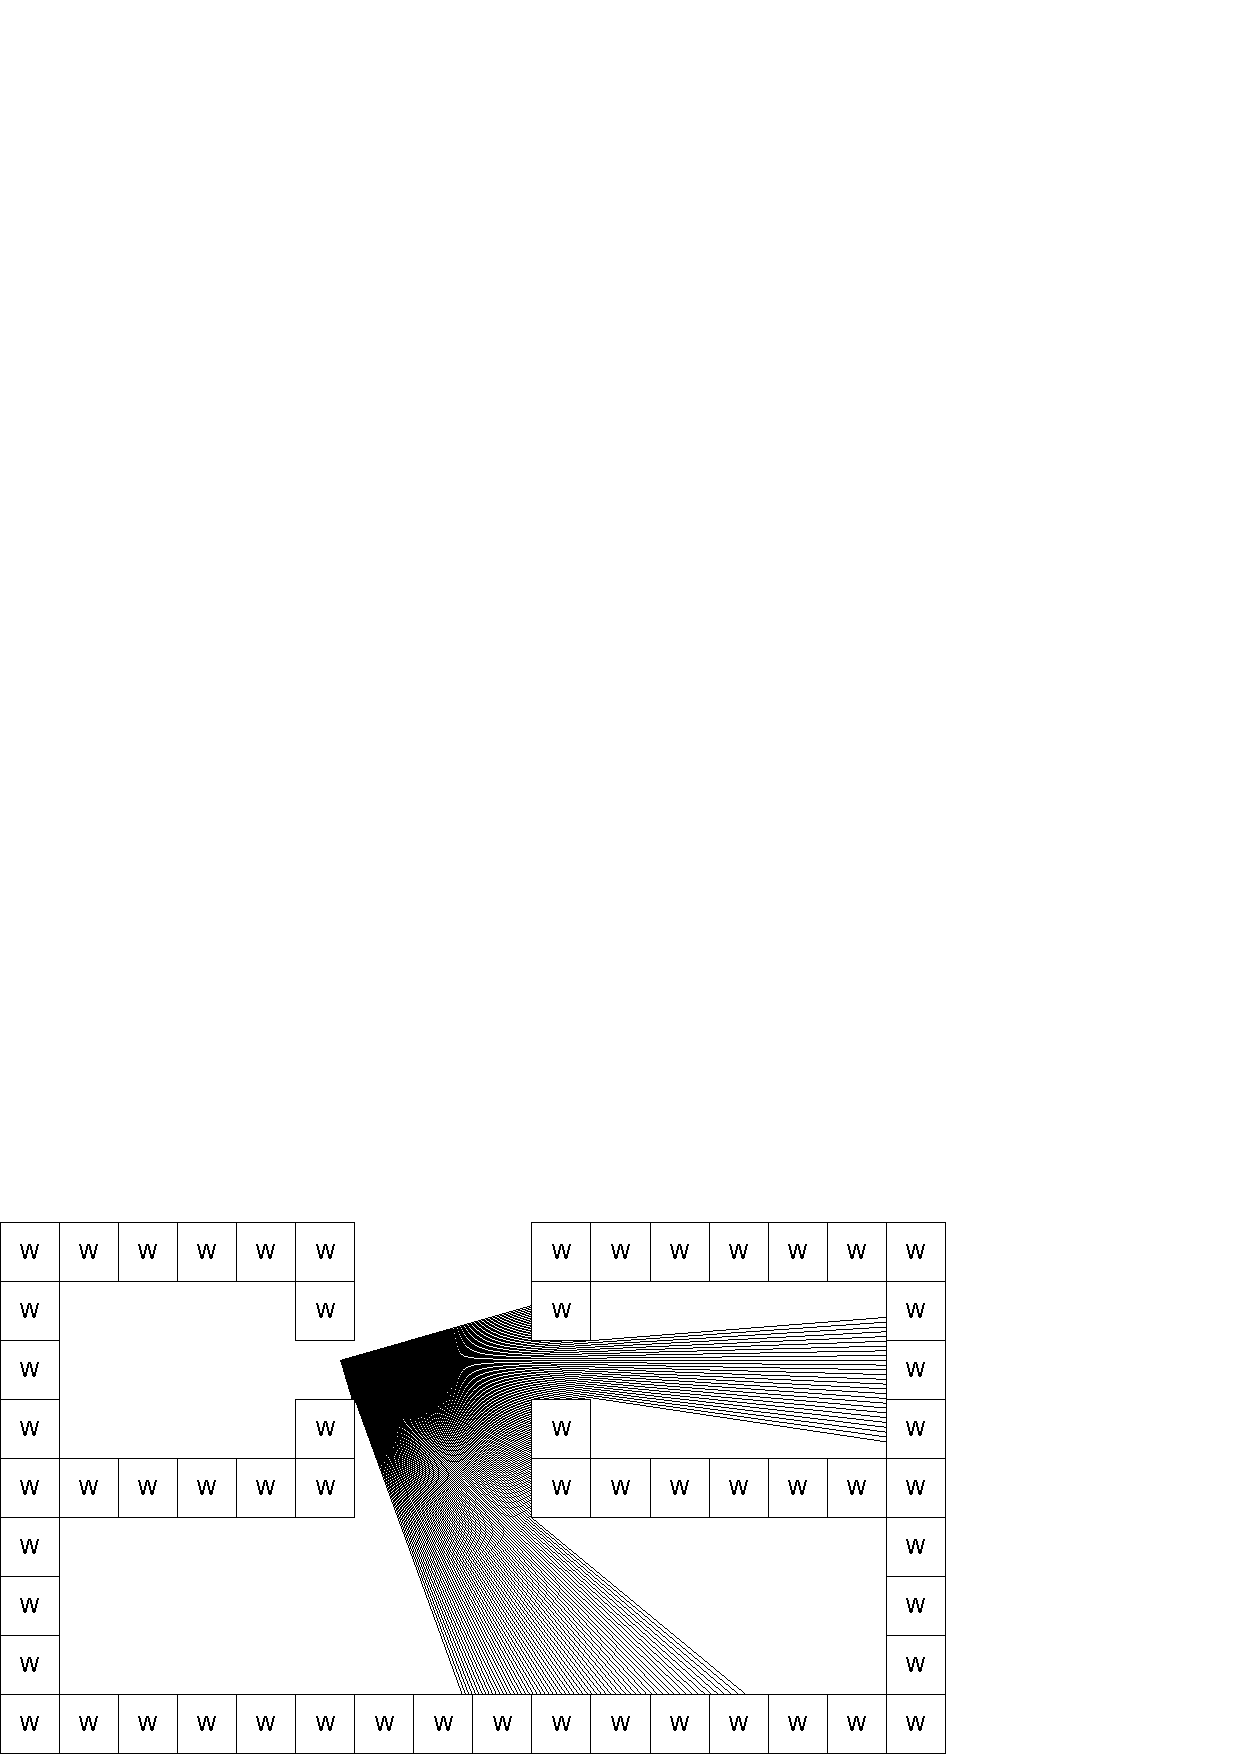
\includegraphics[width=\textwidth]{imgs/drawings/ray_caster_explained/out_room.pdf}
 \caption{Casting 320 rays (one for each column) for a screen of resolution 320x200} \label{fig:Raycasting2}
\end{figure}

\begin{figure}[H]
  \centering
 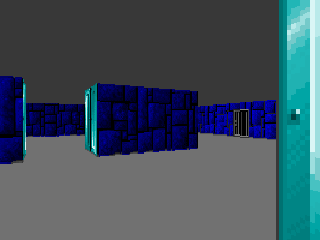
\includegraphics[width=\textwidth]{imgs/drawings/ray_caster_explained/out_door.png}
 \caption{Rendition of the 320 column of pixels (with texturing).} 
\end{figure} 


\subsection{Life of a frame}
As we saw when we unrolled the loop, the action scene is made of frames in a loop which in pseudo code look as follows:\\
\par
\begin{minipage}{\textwidth}
 \lstinputlisting[language=C]{code/flawded_game_loop.c}
 \end{minipage}
\par
This is a pretty standard design for an engine from the early 90. However it has a major flaw. Each slice of the game has a different duration depending on how long it took to render and update the word. This variability makes the game nondeterministic from one machine to an other. Or even between two runs on the same machine as a matter of fact. In the next drawing, all three timeslice representing three frames have different durations.\\
\begin{figure}[H]
\centering
 \includegraphics[width=\textwidth]{imgs/drawings/timer/wrong.pdf}
 
 \end{figure}
  At the beginning of each frame, the engine retrives user inputs and combine them to the duration of the previous frame to update the world. Even if inputs are recorded for each frame, the same game could not be replayed. Because upon replaying a recorded game the engine would invariably reach a point where no inputs are available because a frame took longer or shorter to render. A simple disk access taking longer could have altered the duration of a frame, resulting in a different world outcome.\\
 \begin{figure}[H]
\centering
 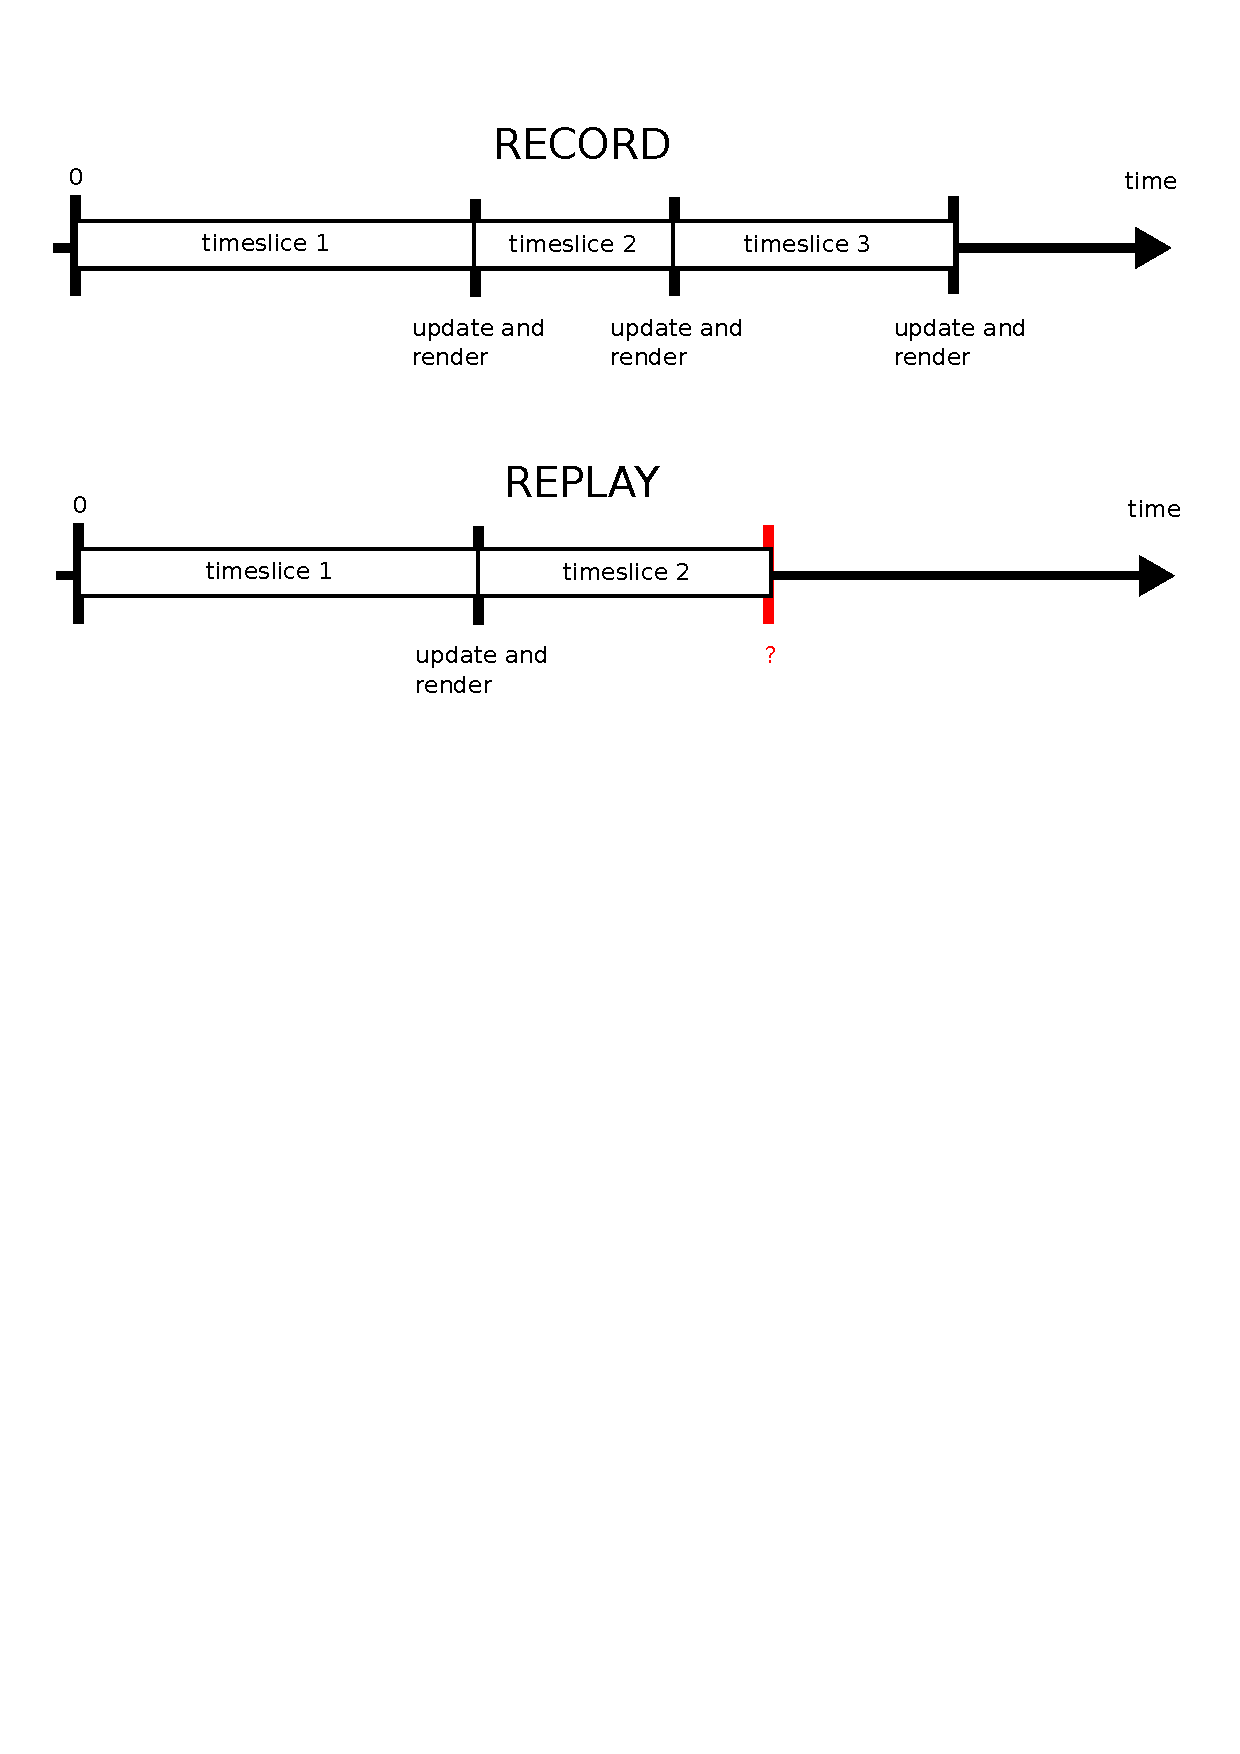
\includegraphics[width=\textwidth]{imgs/drawings/timer/replay.pdf}
 \caption{The second frame rendered faster than during recording. No inputs are available for the player. Replay is now out of sync.}
 \end{figure}
\par
To solve this problem during the demo playback (shipped with the game), the engine disregards the heartbeats and simulate things at fixed timesteps. This hack result in a slower playback on 286 CPUs and faster playback on 486 CPUs (because it was recorded on a 386DX).\\
\par
In 1993, the Doom engine would solve this issue by simulating the world at fixed intervals.\\
\par
\begin{minipage}{\textwidth}
 \lstinputlisting[language=C]{code/fixed_game_loop.c}
 \end{minipage}
\par
This design decouple the renderer from the world updates. Timeslices are always the same duration. User inputs can be recorded and replayed without getting out of sync.
\par
 \begin{figure}[H]
\centering
 \includegraphics[width=\textwidth]{imgs/drawings/timer/fixed.pdf}
 
 \end{figure}

\subsection{Life of a 3D frame}
Before diving into details, here is an overview of the five stages involved in drawing a 3D scene.\\
\begin{enumerate}
 \item Clear the framebuffer by drawing the floor and the ceiling (both solid color).
 \item For each column of pixel on screen, cast a ray from the player to the nearest wall. Draw a textured column of pixels with height inversely proportional to the distance.
 \item Draw the sprites (enemies, lamps, barrels).
 \item Draw the weapon\footnote{A modern 3D engine would render the weapon first and leverage the depth buffer to save fillrate. In that era, memory access were so slow is was faster to accept a little bit of overdraw.}.	
 \item Flip buffers: Instruct CRT Controller to use the framebuffer just composed on next vsync.
\end{enumerate}
In the next six screenshots, the engine has been modified to slow down in order to see the content of the framebuffer at the end of each stage.\\
\begin{figure}[H]
\centering
 \fullimage{wolf3d_1_background.png}
 \caption{Phase 1: Clear screen}
 \end{figure}




\begin{figure}[H]
 \centering
  \fullimage{wolf3d_4_partial_wall_32rays.png}
  \caption{Phase 2: Drawing Walls: 15 rays} 
\end{figure}
\begin{minipage}{.4\textwidth}
Notice how the length of each ray corresponds to the height of a column in order to achieve perspective.\\
\par
The longer the distance the ray traveled, the smaller the column is drawn on screen.
 \end{minipage}
\begin{minipage}{.6\textwidth}
\begin{figure}[H]
  \centering
 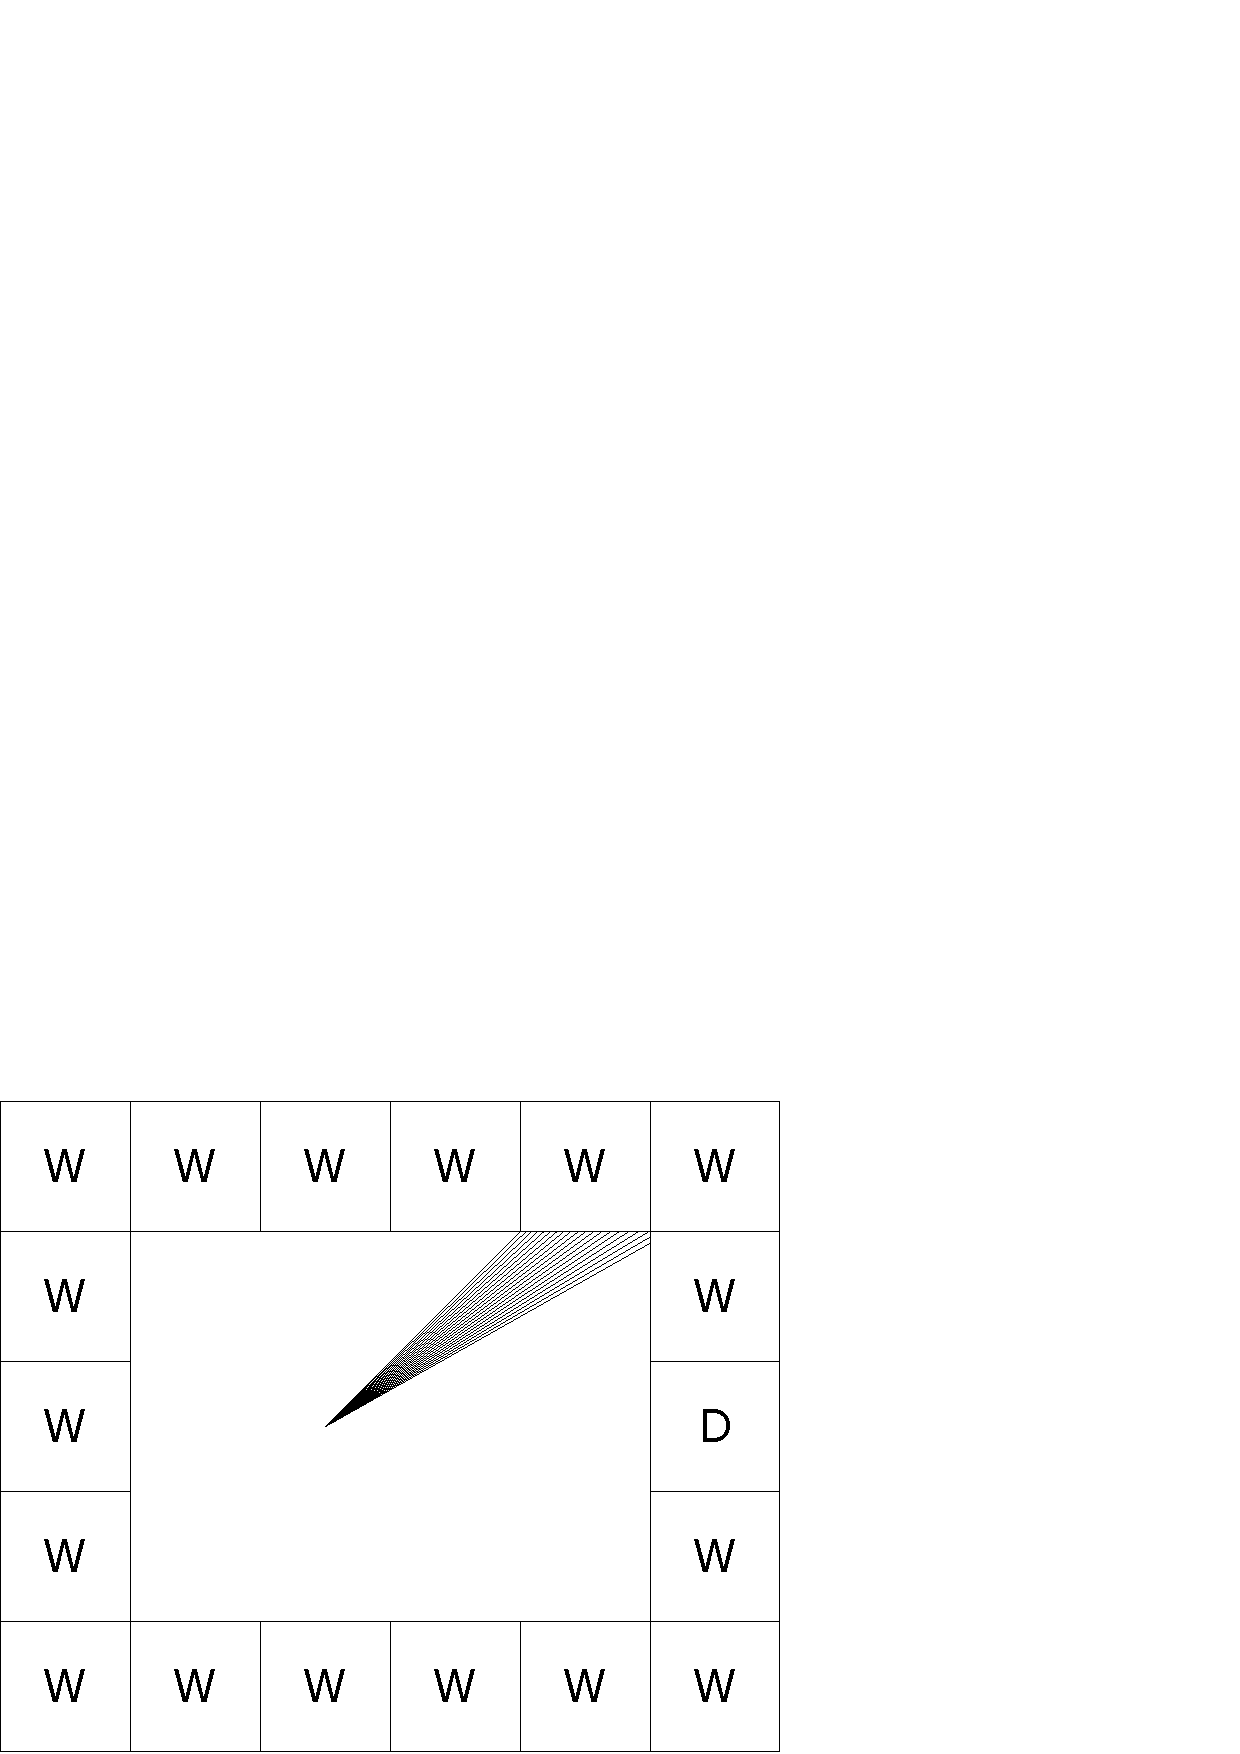
\includegraphics[width=.9\textwidth]{imgs/drawings/ray_caster_explained/beginning10.pdf}
   
\end{figure}
\end{minipage}




 
\begin{figure}[H]
 \centering
  \fullimage{wolf3d_5_partialwalls_160rays.png}
 \caption{Phase 2: Drawing Walls: 160 rays}  
\end{figure}
 \begin{minipage}{.4\textwidth}
 Doors are not sprites, they are part of the solid world. Notice how on the map a door is a block aligned with the wall yet it is rendered farther.\\
 \par
 The raycaster recognize door tiles and inject a delta to the distance a ray traveled. If the door is partially open, the raycaster is also able to detect if the ray should stop or allowed to traverse the tile.
 \end{minipage}
\begin{minipage}{.6\textwidth}
\begin{figure}[H]
  \centering
 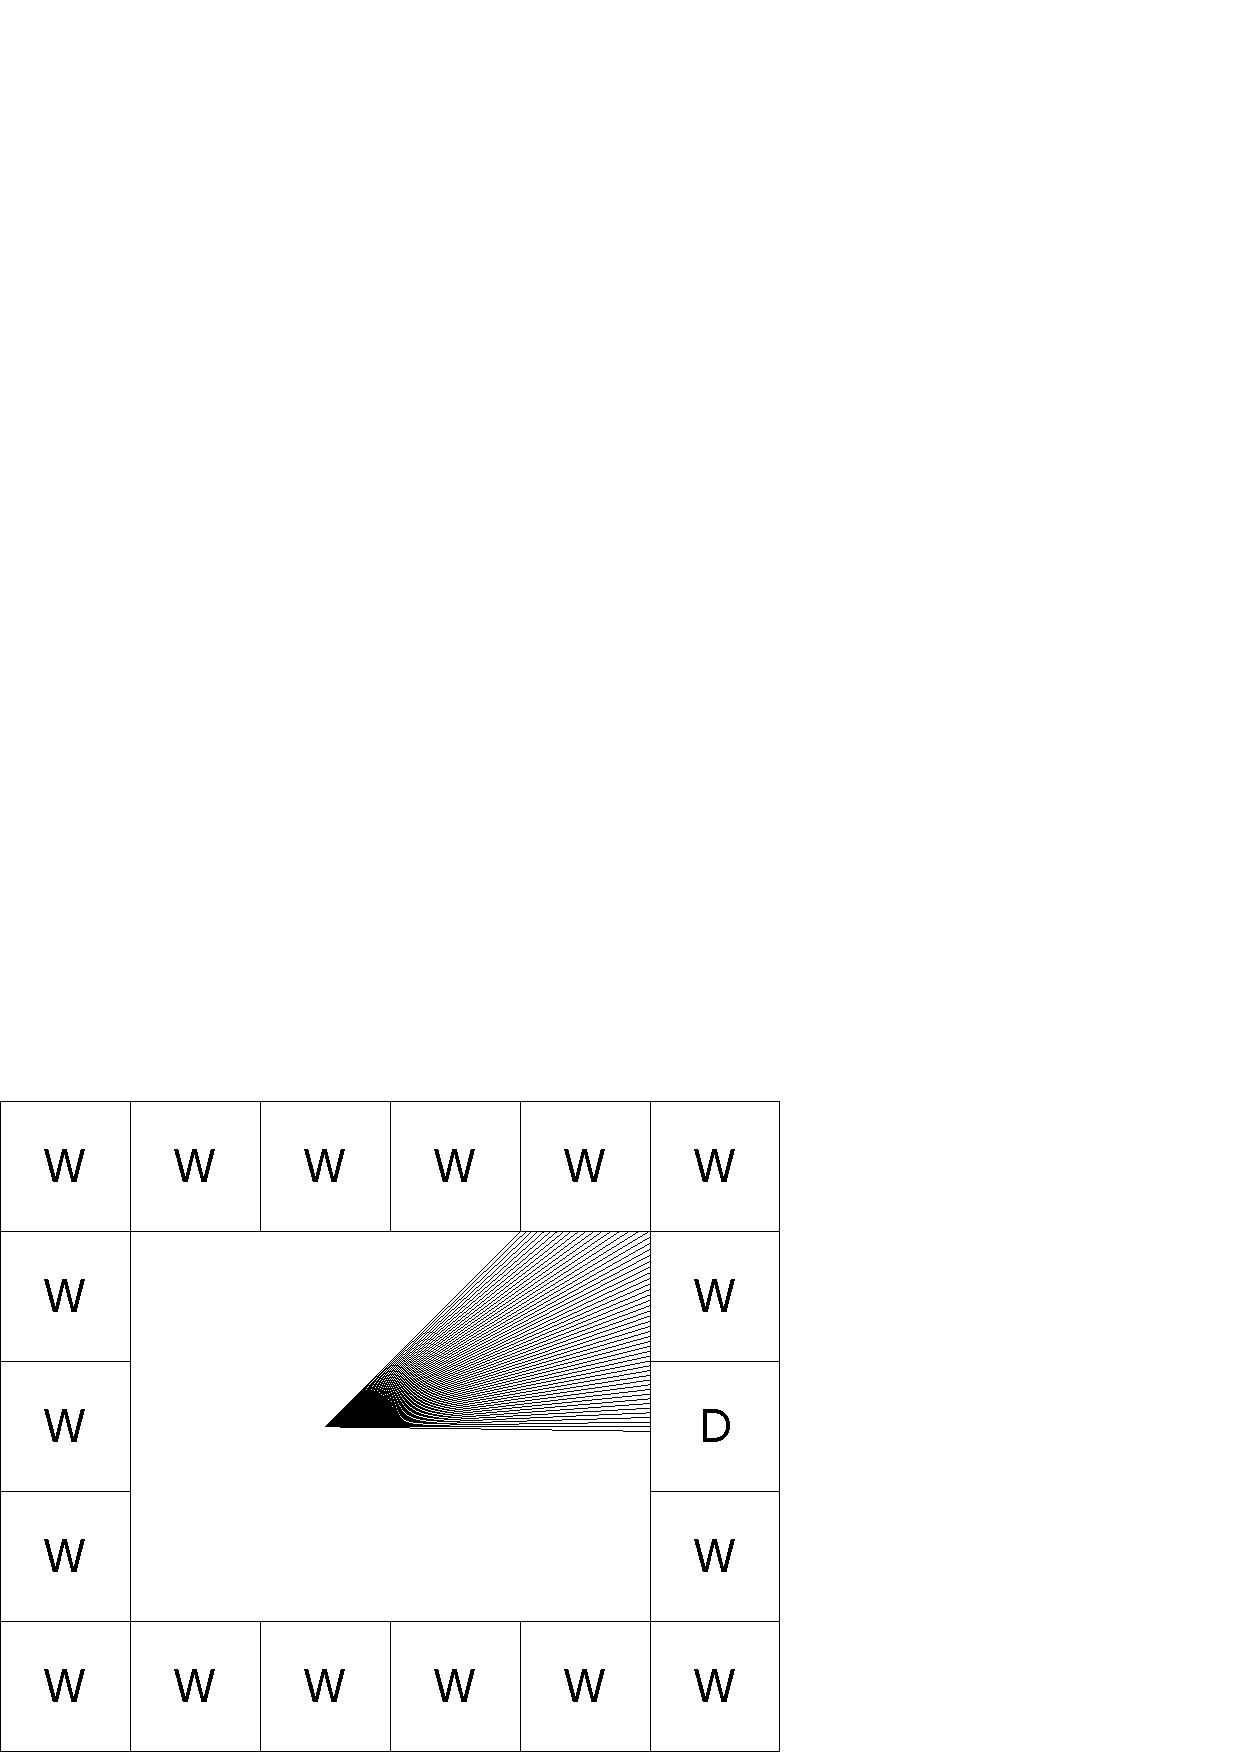
\includegraphics[width=.9\textwidth]{imgs/drawings/ray_caster_explained/beginning50.pdf}
   
\end{figure}
\end{minipage}



 
 \begin{figure}[H]
\centering
 \fullimage{wolf3d_2_walls.png}
 \caption{Phase 2: Drawing Walls has completed.} 
 \end{figure}
\begin{minipage}{\textwidth}
\begin{figure}[H]
  \centering
 
\includegraphics[width=.5\textwidth]{imgs/drawings/ray_caster_explained/beginning.pdf}
   
\end{figure}
\end{minipage}




 
 
 \begin{figure}[H]
\centering
 \fullimage{wolf3d_6_scaled}
 \caption{Phase 3: Drawing Things (a.k.a: Scaled, a.k.a: Sprites)} 
 \end{figure}
 After the raycaster is done, "things" are rendered. During this step, clipping is performed against the wall and doors.




 \begin{figure}[H]
\centering
 \fullimage{wolf3d_7_fullframe.png}
 \caption{Phase 4: Drawing Weapon} 
 \end{figure}
 













\subsection{3D setup}
Before starting to draw frames, the 3D renderer sets up the VRAM with static elements. The 3D view is not fullscreen but contained in a HUD\footnote{Head-up display}.
\begin{figure}[H]
  \centering
 \fullimage{hud_empty.png}
\end{figure}
This HUD is drawn only once at the beginning of the 3D phase. It has to be drawn in all three pages. For each new frame, the engine will draw the 3D view in the reserved white canvas in the center. Small portions at the bottom of the HUD are updated: Level, Score, Lives, Status, Health, Ammo, and Current weapon get a special treatment via an other VGA trick in order to speed up rendition.\\
\par

The hardware chapter described the Mode 12h which despite being unfit for games still had an interesting charcteristic. Mode 12h is a 16 color mode where each pixel color index is contained in a nibble. The four bits are spread across the four VGA banks. Since all write operation are one byte wide, it is not hard to imagine the difficulty to plot a single pixel without changing the other stored in the same bytes. One would have to do four read, four xor and four writes. Since the designer of the VGA were not complete sadist they added some circuitry to simplify this operation. For each bank, they created a latch placed in front of a configurable ALU.\\
\par
 \begin{figure}[H]
\centering
 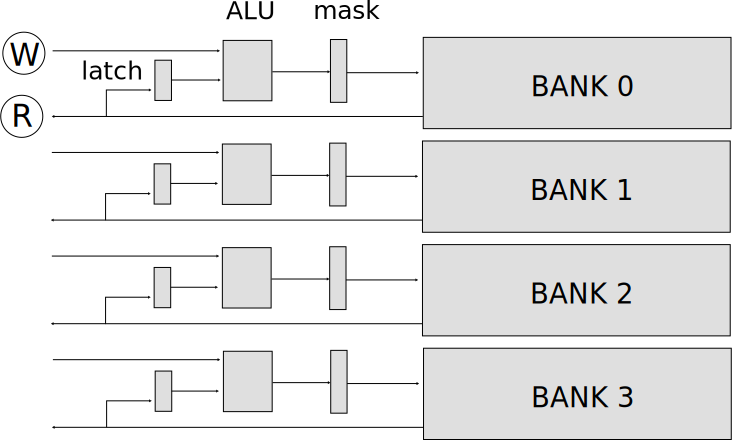
\includegraphics[width=\textwidth]{imgs/drawings/latches.pdf}
 \end{figure}
With this architecture, each time the VRAM is read, the latch from the corresponding bank is loaded with the read value. And each time a value is written to the VRAM, it can be composited by the ALU using the latched value and the written value. This design allowed mode 12h programmers to set a bit in a byte easily with one read, one ALU setup and one write.\\
\par
Mode Y does not need latches to operate since values are stored in bytes and banks can be updated individually thanks to the mask. However tinkerers\footnote{Michael Abrash Grahic Programming Black Book: Chapter 48 -- Mode X Marks the Latch} found that these latches are still active in  Mode-Y. By getting a little bit creative, the circuitry can be repurposed. The ALU in from of each bank can be setup to use only the latch for writing. With such a setup, upon doing one read, four latches are populated at once. And four bytes in the bank are written with only one write to the RAM. This system allows transfer from RAM to VRAM 4 bytes at a time.\\
\par
To take full advantage of this optimization, the 3D renderer uploads images to the VRAM above the fourth page. In total, the 43 sprites used to update the HUD are loaded in the asset page when the engine starts up.\\

\begin{minipage}{.23\textwidth}
     \fullimage{latched/91.png}
  \end{minipage}
\begin{minipage}{.23\textwidth}
     \fullimage{latched/92.png}
  \end{minipage}
\begin{minipage}{.23\textwidth}
     \fullimage{latched/93.png}
  \end{minipage}
\begin{minipage}{.23\textwidth}
     \fullimage{latched/94.png}
  \end{minipage}
\par


\begin{minipage}{.095\textwidth}
     \fullimage{latched/99.png}
  \end{minipage}
\begin{minipage}{.095\textwidth}
     \fullimage{latched/100.png}
  \end{minipage}
\begin{minipage}{.095\textwidth}
     \fullimage{latched/101.png}
  \end{minipage}
\begin{minipage}{.095\textwidth}
     \fullimage{latched/102.png}
  \end{minipage}
\begin{minipage}{.095\textwidth}
     \fullimage{latched/103.png}
  \end{minipage}
\begin{minipage}{.095\textwidth}
     \fullimage{latched/104.png}
  \end{minipage}
\begin{minipage}{.095\textwidth}
     \fullimage{latched/105.png}
  \end{minipage}
\begin{minipage}{.095\textwidth}
     \fullimage{latched/106.png}
  \end{minipage}
\begin{minipage}{.095\textwidth}
     \fullimage{latched/107.png}
  \end{minipage}
\begin{minipage}{.095\textwidth}
     \fullimage{latched/108.png}
  \end{minipage}
\par


\begin{minipage}{.3\textwidth}
     \fullimage{latched/109.png}
  \end{minipage}
\begin{minipage}{.3\textwidth}
     \fullimage{latched/110.png}
  \end{minipage}
\begin{minipage}{.3\textwidth}
     \fullimage{latched/111.png}
  \end{minipage}
\par



\begin{minipage}{.3\textwidth}
     \fullimage{latched/112.png}
  \end{minipage}
\begin{minipage}{.3\textwidth}
     \fullimage{latched/113.png}
  \end{minipage}
\begin{minipage}{.3\textwidth}
     \fullimage{latched/114.png}
  \end{minipage}
\par



  \begin{minipage}{.3\textwidth}
     \fullimage{latched/115.png}
  \end{minipage}
\begin{minipage}{.3\textwidth}
     \fullimage{latched/116.png}
  \end{minipage}
\begin{minipage}{.3\textwidth}
     \fullimage{latched/117.png}
  \end{minipage}
\par





  \begin{minipage}{.3\textwidth}
     \fullimage{latched/118.png}
  \end{minipage}
\begin{minipage}{.3\textwidth}
     \fullimage{latched/119.png}
  \end{minipage}
\begin{minipage}{.3\textwidth}
     \fullimage{latched/120.png}
  \end{minipage}
\par



  \begin{minipage}{.3\textwidth}
     \fullimage{latched/121.png}
  \end{minipage}
\begin{minipage}{.3\textwidth}
     \fullimage{latched/122.png}
  \end{minipage}
\begin{minipage}{.3\textwidth}
     \fullimage{latched/123.png}
  \end{minipage}
\par

    \begin{minipage}{.3\textwidth}
     \fullimage{latched/124.png}
  \end{minipage}
\begin{minipage}{.3\textwidth}
     \fullimage{latched/125.png}
  \end{minipage}
\begin{minipage}{.3\textwidth}
     \fullimage{latched/126.png}
  \end{minipage}
\par

    \begin{minipage}{.3\textwidth}
     \fullimage{latched/127.png}
  \end{minipage}
\begin{minipage}{.3\textwidth}
     \fullimage{latched/128.png}
  \end{minipage}
\begin{minipage}{.3\textwidth}
     \fullimage{latched/129.png}
  \end{minipage}
\par

    \begin{minipage}{.3\textwidth}
     \fullimage{latched/130.png}
  \end{minipage}
\begin{minipage}{.3\textwidth}
     \fullimage{latched/131.png}
  \end{minipage}
\begin{minipage}{.3\textwidth}
     \fullimage{latched/132.png}
  \end{minipage}
\par


\begin{minipage}{.1\textwidth}
     \fullimage{latched/95.png}
  \end{minipage}
\begin{minipage}{.1\textwidth}
     \fullimage{latched/96.png}
  \end{minipage}
\begin{minipage}{.1\textwidth}
     \fullimage{latched/97.png}
  \end{minipage}
\begin{minipage}{.1\textwidth}
     \fullimage{latched/98.png}
  \end{minipage}
  \begin{minipage}{.3\textwidth}
     \fullimage{latched/133.png}
  \end{minipage}
\begin{minipage}{.3\textwidth}
     \fullimage{latched/134.png}
  \end{minipage}\

\bu{Tick :} Images are stored woven. All bytes for bank 0 first, then all bytes for bank 1 and so on. This clever way to store data allow a bank to be loaded very fast with one single \cw{memcpy} (four \cw{memcpy} per image).\\
\par
All these assets account for 48*24*4 (weapons sprites) + 14*8*16 (numerals and keys sprites) + 24*24*32 (faces sprites) + 224 * 48 (paused + psyched) = 34,816 bytes. There are therefore 27,648 unused bytes in the fourth VGA page.\\
\par
For this trick to work, images source and destination have to be aligned on four byte horizontally in screen space. If you take a look at the location of each elements on screen you can see that elements are aligned on four pixels horizontally but there is no such constraint vertically.
\begin{figure}[H]
  \centering
 \includegraphics[width=\textwidth]{imgs/drawings/hud.pdf}
\end{figure}

While it is faster to write four pixel in one operation, the trick does not provide a full 400\% speed increase since all writes have to be done in all three screen pages. It is obvious when looking at the routine updating the status (hero's face).\\
\par
\begin{minipage}{\textwidth}
\lstinputlisting[language=C]{code/StatusDrawPic.c}
\end{minipage}



\subsection{Clearing the screen}
At the beginning of a frame, the engine switches to the next page and clears the 3D area with ceiling and floor colors. To this effect, it uses the same trick seen in the 2D renderer and sets the VGA bank mask to 15 to write to all banks simultaneously. Again, since values are written 16 bits at a time it can write 8 pixels at a time.\\ 
\par
\begin{minipage}{\textwidth}
 \lstinputlisting[language=C,morekeywords=asm]{code/VGAClearScreen.c}
 \end{minipage}
\par
Clearing the 3D canvas made of 304*152=46,208 pixels requires only 46,208/8 = 5776 write operations.\\
\par
The colors for the floor and the ceiling do not come from the maps data files. The ground is always the same color (\cw{0x19}) and the ceiling colors are hardcoded in the engine on a per level basis.\\
\par
\begin{minipage}{\textwidth}
 \lstinputlisting[language=C,morekeywords=byte]{code/vgaCeiling.c}
 \end{minipage}
\par


Following, ceiling colors \cw{0x1D}, \cw{0xBF}, \cw{0x4E} and \cw{0x8D}.\\ 
\par
\scaledimage{.24}{palette_1d.png}
\scaledimage{.24}{palette_bf.png}
\scaledimage{.24}{palette_8d.png}
\scaledimage{.24}{palette_4e.png}






\subsection{Solving the CPU problem}

The hardware chapter describing the CPU capabilities had left the reader with a problem at hands: The machine cannot do floating point operations fast enough. This is a pretty big deal for a 3D engine and all the trigonometry involved. It turns out the solution is to trick the ALU via a technique called "fixed point arithmetic".







\subsubsection{Fixed point}
The normal layout of an \cw{int} is as follow.
\begin{figure}[H]
\centering
 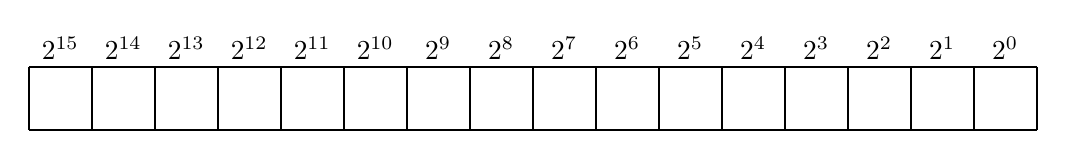
\begin{tikzpicture}[scale=0.8, every node/.style={scale=0.99}]
\draw[thick] (0,0) -- (16,0);
\draw[thick] (0,1) -- (16,1);
\foreach \i in {0,...,16}
{
     \draw[thick] (\i,1) -- (\i,0);
}

\foreach \i in {0,...,15}
{
     \node[] at (15-\i+0.5,1.3){$2^{\i}$}  ;
       
       
     
}
\end{tikzpicture}

 \caption{Integer layout.} \label{fig:int_layout}
 \end{figure}
The value of the sequence of bits \emph{0010010010010010}:
\begin{figure}[H]
\centering
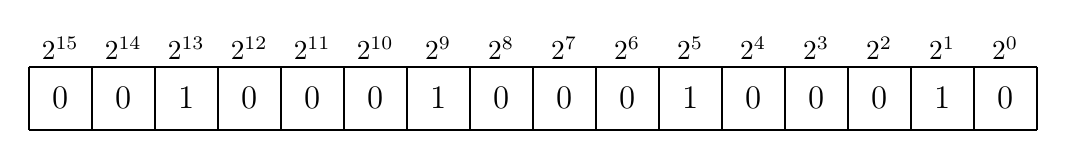
\begin{tikzpicture}[scale=0.8, every node/.style={scale=0.99}]
\draw[thick] (0,0) -- (16,0);
\draw[thick] (0,1) -- (16,1);
\foreach \i in {0,...,16}
{
     \draw[thick] (\i,1) -- (\i,0);
}

\foreach \i in {0,...,15}
{
     \node[] at (15-\i+0.5,1.3){$2^{\i}$}  ;
}

\tikzstyle{fontbf} = [font=\large]
\node[fontbf] at (0.5,0.5){0} ;
\node[fontbf] at (1.5,0.5){0};  
\node[fontbf] at (2.5,0.5){1} ; 
\node[fontbf] at (3.5,0.5){0} ;

\node[fontbf] at (4.5,0.5){0} ;
\node[fontbf] at (5.5,0.5){0};  
\node[fontbf] at (6.5,0.5){1} ; 
\node[fontbf] at (7.5,0.5){0} ;

\node[fontbf] at (8.5,0.5){0} ;
\node[fontbf] at (9.5,0.5){0};  
\node[fontbf] at (10.5,0.5){1} ; 
\node[fontbf] at (11.5,0.5){0} ;

\node[fontbf] at (12.5,0.5){0} ;
\node[fontbf] at (13.5,0.5){0};  
\node[fontbf] at (14.5,0.5){1} ; 
\node[fontbf] at (15.5,0.5){0} ;


\end{tikzpicture}

 \end{figure}

Represents $ 2^{13} + 2^9 + 2^5 + 2^1 =  8738 $.\\
 \par

Fixed Point allows to keep track of fractions while still using the integer operations of the CPU. The machine manipulates what are supposed to be integer numbers but the programmers sees them as a value containing an integer part and a fractional part:\\
\par
\begin{figure}[H]
 \centering
  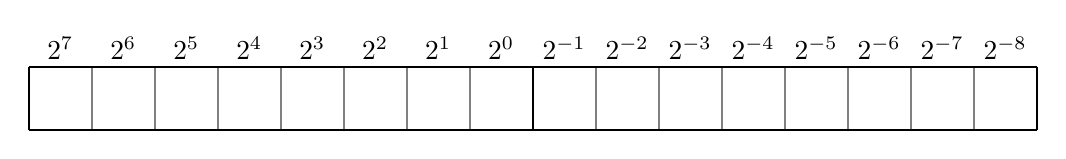
\begin{tikzpicture}[scale=0.8, every node/.style={scale=0.99}]


\colorlet{LighterMark}{black!50}

\foreach \i in {1,...,15}
{
     \draw[thick,LighterMark] (\i,1) -- (\i,0);
}

     \draw[thick,black] (0,1) -- (0,0);
      \draw[thick,black] (8,1) -- (8,0);
      \draw[thick,black] (16,1) -- (16,0);
      
\draw[thick,black] (0,0) -- (16,0);
\draw[thick,black] (0,1) -- (16,1);
 

%\foreach \i[evaluate={\pow=int(7-\i)}] in {0,...,7}
\foreach \i[evaluate={\pow=int(7-\i)}] in {0,...,7}
{
   \node[] at (\i+0.5,1.3){$2^{\pow}$  }  ;
      
         
     
}

%\foreach \i[evaluate={\pow=int((\i-7)*2)}]  in {8,...,15}
\foreach \i[evaluate={\pow=int(\i-7)}]  in {8,...,15}
{
     \node[] at (\i+0.5,1.3){$2^{-\pow}$}  ;
}




\end{tikzpicture}

 \caption{Fixed point layout 8:8 (8-bits for the integer part and 8 bits for the fractional part).} \label{fig:mips}
\end{figure}

The same sequence of bits \emph{0010010010010010} with different powers of two...
\begin{figure}[H]
 \centering
   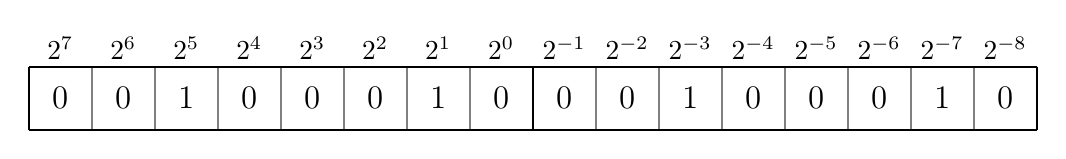
\begin{tikzpicture}[scale=0.8, every node/.style={scale=0.99}]


\colorlet{LighterMark}{black!50}

\foreach \i in {1,...,15}
{
     \draw[thick,LighterMark] (\i,1) -- (\i,0);
}

     \draw[thick,black] (0,1) -- (0,0);
      \draw[thick,black] (8,1) -- (8,0);
      \draw[thick,black] (16,1) -- (16,0);
      
\draw[thick,black] (0,0) -- (16,0);
\draw[thick,black] (0,1) -- (16,1);
 

%\foreach \i[evaluate={\pow=int(7-\i)}] in {0,...,7}
\foreach \i[evaluate={\pow=int(7-\i)}] in {0,...,7}
{
   \node[] at (\i+0.5,1.3){$2^{\pow}$  }  ;
      
         
     
}

%\foreach \i[evaluate={\pow=int((\i-7)*2)}]  in {8,...,15}
\foreach \i[evaluate={\pow=int(\i-7)}]  in {8,...,15}
{
     \node[] at (\i+0.5,1.3){$2^{-\pow}$}  ;
}

\tikzstyle{fontbf} = [font=\large]
\node[fontbf] at (0.5,0.5){0} ;
\node[fontbf] at (1.5,0.5){0};  
\node[fontbf] at (2.5,0.5){1} ; 
\node[fontbf] at (3.5,0.5){0} ;

\node[fontbf] at (4.5,0.5){0} ;
\node[fontbf] at (5.5,0.5){0};  
\node[fontbf] at (6.5,0.5){1} ; 
\node[fontbf] at (7.5,0.5){0} ;

\node[fontbf] at (8.5,0.5){0} ;
\node[fontbf] at (9.5,0.5){0};  
\node[fontbf] at (10.5,0.5){1} ; 
\node[fontbf] at (11.5,0.5){0} ;

\node[fontbf] at (12.5,0.5){0} ;
\node[fontbf] at (13.5,0.5){0};  
\node[fontbf] at (14.5,0.5){1} ; 
\node[fontbf] at (15.5,0.5){0} ;


\end{tikzpicture}

\end{figure} 

Now represents:\\

$ 2^5 + 2^1 = 34 $ for the integer part.\\
$ 2^{-3}+2^{-7} = 0.1328125 $ for the fractional part.\\
$ = 34.1328125$\\

\bigskip

The beauty of fixed point is that addition and subtraction work exactly like integers from the CPU instruction side.\\




\par
\begin{figure}[H]
 \centering
   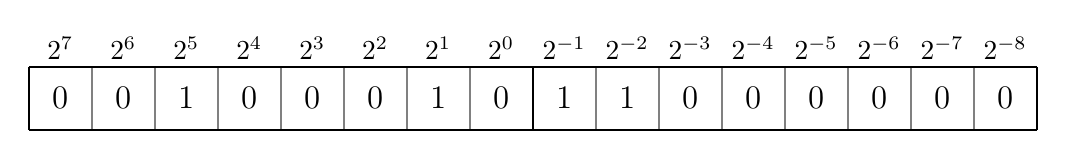
\begin{tikzpicture}[scale=0.8, every node/.style={scale=0.99}]


\colorlet{LighterMark}{black!50}

\foreach \i in {1,...,15}
{
     \draw[thick,LighterMark] (\i,1) -- (\i,0);
}

     \draw[thick,black] (0,1) -- (0,0);
      \draw[thick,black] (8,1) -- (8,0);
      \draw[thick,black] (16,1) -- (16,0);
      
\draw[thick,black] (0,0) -- (16,0);
\draw[thick,black] (0,1) -- (16,1);
 

%\foreach \i[evaluate={\pow=int(7-\i)}] in {0,...,7}
\foreach \i[evaluate={\pow=int(7-\i)}] in {0,...,7}
{
   \node[] at (\i+0.5,1.3){$2^{\pow}$  }  ;
      
         
     
}

%\foreach \i[evaluate={\pow=int((\i-7)*2)}]  in {8,...,15}
\foreach \i[evaluate={\pow=int(\i-7)}]  in {8,...,15}
{
     \node[] at (\i+0.5,1.3){$2^{-\pow}$}  ;
}

\tikzstyle{fontbf} = [font=\large]
\node[fontbf] at (0.5,0.5){0} ;
\node[fontbf] at (1.5,0.5){0};  
\node[fontbf] at (2.5,0.5){1} ; 
\node[fontbf] at (3.5,0.5){0} ;

\node[fontbf] at (4.5,0.5){0} ;
\node[fontbf] at (5.5,0.5){0};  
\node[fontbf] at (6.5,0.5){1} ; 
\node[fontbf] at (7.5,0.5){0} ;

\node[fontbf] at (8.5,0.5){1} ;
\node[fontbf] at (9.5,0.5){1};  
\node[fontbf] at (10.5,0.5){0} ; 
\node[fontbf] at (11.5,0.5){0} ;

\node[fontbf] at (12.5,0.5){0} ;
\node[fontbf] at (13.5,0.5){0};  
\node[fontbf] at (14.5,0.5){0} ; 
\node[fontbf] at (15.5,0.5){0} ;


\end{tikzpicture}


   \caption{34.75} 
\end{figure} 

\begin{figure}[H]
 \centering
   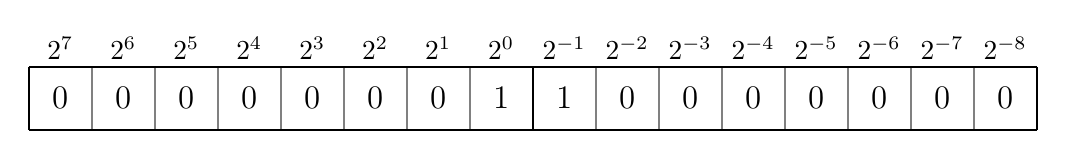
\begin{tikzpicture}[scale=0.8, every node/.style={scale=0.99}]


\colorlet{LighterMark}{black!50}

\foreach \i in {1,...,15}
{
     \draw[thick,LighterMark] (\i,1) -- (\i,0);
}

     \draw[thick,black] (0,1) -- (0,0);
      \draw[thick,black] (8,1) -- (8,0);
      \draw[thick,black] (16,1) -- (16,0);
      
\draw[thick,black] (0,0) -- (16,0);
\draw[thick,black] (0,1) -- (16,1);
 

%\foreach \i[evaluate={\pow=int(7-\i)}] in {0,...,7}
\foreach \i[evaluate={\pow=int(7-\i)}] in {0,...,7}
{
   \node[] at (\i+0.5,1.3){$2^{\pow}$  }  ;
      
         
     
}

%\foreach \i[evaluate={\pow=int((\i-7)*2)}]  in {8,...,15}
\foreach \i[evaluate={\pow=int(\i-7)}]  in {8,...,15}
{
     \node[] at (\i+0.5,1.3){$2^{-\pow}$}  ;
}

\tikzstyle{fontbf} = [font=\large]
\node[fontbf] at (0.5,0.5){0} ;
\node[fontbf] at (1.5,0.5){0};  
\node[fontbf] at (2.5,0.5){0} ; 
\node[fontbf] at (3.5,0.5){0} ;

\node[fontbf] at (4.5,0.5){0} ;
\node[fontbf] at (5.5,0.5){0};  
\node[fontbf] at (6.5,0.5){0} ; 
\node[fontbf] at (7.5,0.5){1} ;

\node[fontbf] at (8.5,0.5){1} ;
\node[fontbf] at (9.5,0.5){0};  
\node[fontbf] at (10.5,0.5){0} ; 
\node[fontbf] at (11.5,0.5){0} ;

\node[fontbf] at (12.5,0.5){0} ;
\node[fontbf] at (13.5,0.5){0};  
\node[fontbf] at (14.5,0.5){0} ; 
\node[fontbf] at (15.5,0.5){0} ;


\end{tikzpicture}

  \caption{+ 1.5} 
\end{figure} 

\begin{figure}[H]
 \centering
   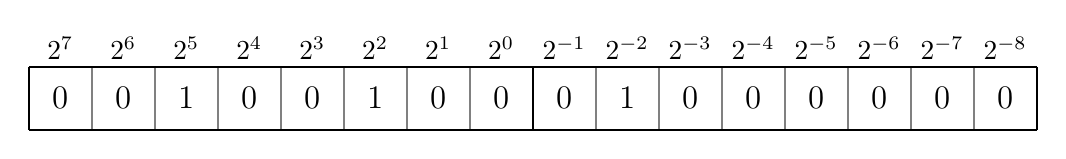
\begin{tikzpicture}[scale=0.8, every node/.style={scale=0.99}]


\colorlet{LighterMark}{black!50}

\foreach \i in {1,...,15}
{
     \draw[thick,LighterMark] (\i,1) -- (\i,0);
}

     \draw[thick,black] (0,1) -- (0,0);
      \draw[thick,black] (8,1) -- (8,0);
      \draw[thick,black] (16,1) -- (16,0);
      
\draw[thick,black] (0,0) -- (16,0);
\draw[thick,black] (0,1) -- (16,1);
 

%\foreach \i[evaluate={\pow=int(7-\i)}] in {0,...,7}
\foreach \i[evaluate={\pow=int(7-\i)}] in {0,...,7}
{
   \node[] at (\i+0.5,1.3){$2^{\pow}$  }  ;
      
         
     
}

%\foreach \i[evaluate={\pow=int((\i-7)*2)}]  in {8,...,15}
\foreach \i[evaluate={\pow=int(\i-7)}]  in {8,...,15}
{
     \node[] at (\i+0.5,1.3){$2^{-\pow}$}  ;
}

\tikzstyle{fontbf} = [font=\large]
\node[fontbf] at (0.5,0.5){0} ;
\node[fontbf] at (1.5,0.5){0};  
\node[fontbf] at (2.5,0.5){1} ; 
\node[fontbf] at (3.5,0.5){0} ;

\node[fontbf] at (4.5,0.5){0} ;
\node[fontbf] at (5.5,0.5){1};  
\node[fontbf] at (6.5,0.5){0} ; 
\node[fontbf] at (7.5,0.5){0} ;

\node[fontbf] at (8.5,0.5){0} ;
\node[fontbf] at (9.5,0.5){1};  
\node[fontbf] at (10.5,0.5){0} ; 
\node[fontbf] at (11.5,0.5){0} ;

\node[fontbf] at (12.5,0.5){0} ;
\node[fontbf] at (13.5,0.5){0};  
\node[fontbf] at (14.5,0.5){0} ; 
\node[fontbf] at (15.5,0.5){0} ;


\end{tikzpicture}

  {\caption{= 36.25}}
\end{figure} 
\par
 Even right shit and left shift trick work...\\
 
 \par
\begin{figure}[H]
 \centering
   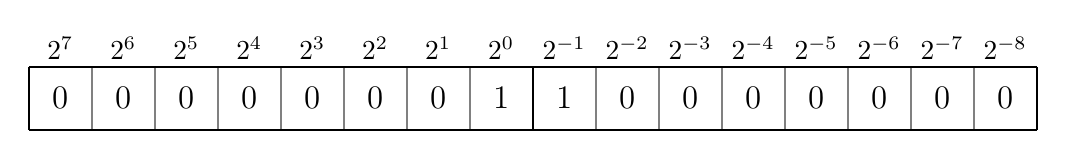
\begin{tikzpicture}[scale=0.8, every node/.style={scale=0.99}]


\colorlet{LighterMark}{black!50}

\foreach \i in {1,...,15}
{
     \draw[thick,LighterMark] (\i,1) -- (\i,0);
}

     \draw[thick,black] (0,1) -- (0,0);
      \draw[thick,black] (8,1) -- (8,0);
      \draw[thick,black] (16,1) -- (16,0);
      
\draw[thick,black] (0,0) -- (16,0);
\draw[thick,black] (0,1) -- (16,1);
 

%\foreach \i[evaluate={\pow=int(7-\i)}] in {0,...,7}
\foreach \i[evaluate={\pow=int(7-\i)}] in {0,...,7}
{
   \node[] at (\i+0.5,1.3){$2^{\pow}$  }  ;
      
         
     
}

%\foreach \i[evaluate={\pow=int((\i-7)*2)}]  in {8,...,15}
\foreach \i[evaluate={\pow=int(\i-7)}]  in {8,...,15}
{
     \node[] at (\i+0.5,1.3){$2^{-\pow}$}  ;
}

\tikzstyle{fontbf} = [font=\large]
\node[fontbf] at (0.5,0.5){0} ;
\node[fontbf] at (1.5,0.5){0};  
\node[fontbf] at (2.5,0.5){0} ; 
\node[fontbf] at (3.5,0.5){0} ;

\node[fontbf] at (4.5,0.5){0} ;
\node[fontbf] at (5.5,0.5){0};  
\node[fontbf] at (6.5,0.5){0} ; 
\node[fontbf] at (7.5,0.5){1} ;

\node[fontbf] at (8.5,0.5){1} ;
\node[fontbf] at (9.5,0.5){0};  
\node[fontbf] at (10.5,0.5){0} ; 
\node[fontbf] at (11.5,0.5){0} ;

\node[fontbf] at (12.5,0.5){0} ;
\node[fontbf] at (13.5,0.5){0};  
\node[fontbf] at (14.5,0.5){0} ; 
\node[fontbf] at (15.5,0.5){0} ;


\end{tikzpicture}

   \caption{1.5} 
\end{figure} 

\par
\begin{figure}[H]
 \centering
   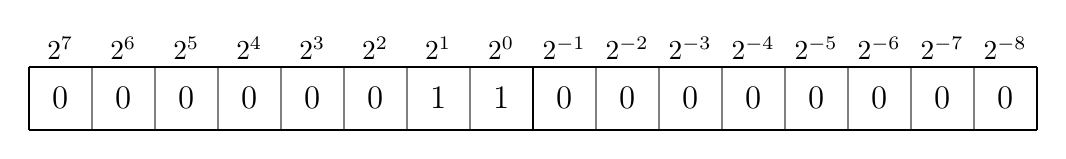
\begin{tikzpicture}[scale=0.8, every node/.style={scale=0.99}]


\colorlet{LighterMark}{black!50}

\foreach \i in {1,...,15}
{
     \draw[thick,LighterMark] (\i,1) -- (\i,0);
}

     \draw[thick,black] (0,1) -- (0,0);
      \draw[thick,black] (8,1) -- (8,0);
      \draw[thick,black] (16,1) -- (16,0);
      
\draw[thick,black] (0,0) -- (16,0);
\draw[thick,black] (0,1) -- (16,1);
 

%\foreach \i[evaluate={\pow=int(7-\i)}] in {0,...,7}
\foreach \i[evaluate={\pow=int(7-\i)}] in {0,...,7}
{
   \node[] at (\i+0.5,1.3){$2^{\pow}$  }  ;
      
         
     
}

%\foreach \i[evaluate={\pow=int((\i-7)*2)}]  in {8,...,15}
\foreach \i[evaluate={\pow=int(\i-7)}]  in {8,...,15}
{
     \node[] at (\i+0.5,1.3){$2^{-\pow}$}  ;
}

\tikzstyle{fontbf} = [font=\large]
\node[fontbf] at (0.5,0.5){0} ;
\node[fontbf] at (1.5,0.5){0};  
\node[fontbf] at (2.5,0.5){0} ; 
\node[fontbf] at (3.5,0.5){0} ;

\node[fontbf] at (4.5,0.5){0} ;
\node[fontbf] at (5.5,0.5){0};  
\node[fontbf] at (6.5,0.5){1} ; 
\node[fontbf] at (7.5,0.5){1} ;

\node[fontbf] at (8.5,0.5){0} ;
\node[fontbf] at (9.5,0.5){0};  
\node[fontbf] at (10.5,0.5){0} ; 
\node[fontbf] at (11.5,0.5){0} ;

\node[fontbf] at (12.5,0.5){0} ;
\node[fontbf] at (13.5,0.5){0};  
\node[fontbf] at (14.5,0.5){0} ; 
\node[fontbf] at (15.5,0.5){0} ;


\end{tikzpicture}

   \caption{1.5 << 2  = 3} 
\end{figure}

\par
\begin{figure}[H]
 \centering
   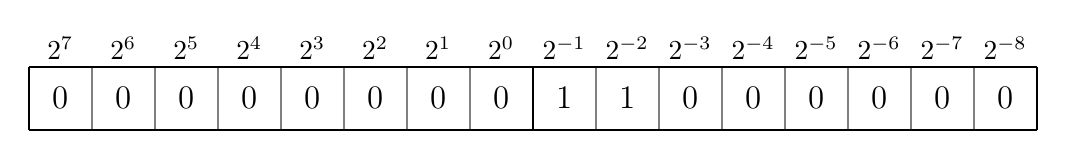
\begin{tikzpicture}[scale=0.8, every node/.style={scale=0.99}]


\colorlet{LighterMark}{black!50}

\foreach \i in {1,...,15}
{
     \draw[thick,LighterMark] (\i,1) -- (\i,0);
}

     \draw[thick,black] (0,1) -- (0,0);
      \draw[thick,black] (8,1) -- (8,0);
      \draw[thick,black] (16,1) -- (16,0);
      
\draw[thick,black] (0,0) -- (16,0);
\draw[thick,black] (0,1) -- (16,1);
 

%\foreach \i[evaluate={\pow=int(7-\i)}] in {0,...,7}
\foreach \i[evaluate={\pow=int(7-\i)}] in {0,...,7}
{
   \node[] at (\i+0.5,1.3){$2^{\pow}$  }  ;
      
         
     
}

%\foreach \i[evaluate={\pow=int((\i-7)*2)}]  in {8,...,15}
\foreach \i[evaluate={\pow=int(\i-7)}]  in {8,...,15}
{
     \node[] at (\i+0.5,1.3){$2^{-\pow}$}  ;
}

\tikzstyle{fontbf} = [font=\large]
\node[fontbf] at (0.5,0.5){0} ;
\node[fontbf] at (1.5,0.5){0};  
\node[fontbf] at (2.5,0.5){0} ; 
\node[fontbf] at (3.5,0.5){0} ;

\node[fontbf] at (4.5,0.5){0} ;
\node[fontbf] at (5.5,0.5){0};  
\node[fontbf] at (6.5,0.5){0} ; 
\node[fontbf] at (7.5,0.5){0} ;

\node[fontbf] at (8.5,0.5){1} ;
\node[fontbf] at (9.5,0.5){1};  
\node[fontbf] at (10.5,0.5){0} ; 
\node[fontbf] at (11.5,0.5){0} ;

\node[fontbf] at (12.5,0.5){0} ;
\node[fontbf] at (13.5,0.5){0};  
\node[fontbf] at (14.5,0.5){0} ; 
\node[fontbf] at (15.5,0.5){0} ;


\end{tikzpicture}

   \caption{1.5 >> 2 = 0.75} 
\end{figure}

The notation for fixed point is \cw{BITS\_FOR\_INTEGER\_PART:BITS\_FOR\_FRACTIONNAL\_PART}. In the game, the player position is \cw{16:16}. The grid location is one shift operation away \cw{player->x $\gg$ 16}.\\
\par
 The special case is when performing multiplication. There are two ways to do it: Either multiply two 32 bits into a 64 bits (and drop the upper and lower 16 bits) or drop the precision of both fixed point and then multiply then into a 32 bits. Both methods involve accepting a loss of data via overflow or underflow. Let's take the example of $98.7539 * 1.5$.


\par
\begin{figure}[H]
 \centering
   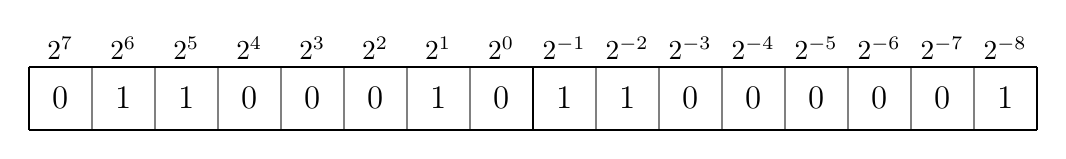
\begin{tikzpicture}[scale=0.8, every node/.style={scale=0.99}]


\colorlet{LighterMark}{black!50}

\foreach \i in {1,...,15}
{
     \draw[thick,LighterMark] (\i,1) -- (\i,0);
}

     \draw[thick,black] (0,1) -- (0,0);
      \draw[thick,black] (8,1) -- (8,0);
      \draw[thick,black] (16,1) -- (16,0);
      
\draw[thick,black] (0,0) -- (16,0);
\draw[thick,black] (0,1) -- (16,1);
 

%\foreach \i[evaluate={\pow=int(7-\i)}] in {0,...,7}
\foreach \i[evaluate={\pow=int(7-\i)}] in {0,...,7}
{
   \node[] at (\i+0.5,1.3){$2^{\pow}$  }  ;
      
         
     
}

%\foreach \i[evaluate={\pow=int((\i-7)*2)}]  in {8,...,15}
\foreach \i[evaluate={\pow=int(\i-7)}]  in {8,...,15}
{
     \node[] at (\i+0.5,1.3){$2^{-\pow}$}  ;
}

\tikzstyle{fontbf} = [font=\large]
\node[fontbf] at (0.5,0.5){0} ;
\node[fontbf] at (1.5,0.5){1};  
\node[fontbf] at (2.5,0.5){1} ; 
\node[fontbf] at (3.5,0.5){0} ;

\node[fontbf] at (4.5,0.5){0} ;
\node[fontbf] at (5.5,0.5){0};  
\node[fontbf] at (6.5,0.5){1} ; 
\node[fontbf] at (7.5,0.5){0} ;

\node[fontbf] at (8.5,0.5){1} ;
\node[fontbf] at (9.5,0.5){1};  
\node[fontbf] at (10.5,0.5){0} ; 
\node[fontbf] at (11.5,0.5){0} ;

\node[fontbf] at (12.5,0.5){0} ;
\node[fontbf] at (13.5,0.5){0};  
\node[fontbf] at (14.5,0.5){0} ; 
\node[fontbf] at (15.5,0.5){1} ;


\end{tikzpicture}

   \caption{98.7539} 
\end{figure} 
\par
\begin{figure}[H]
 \centering
   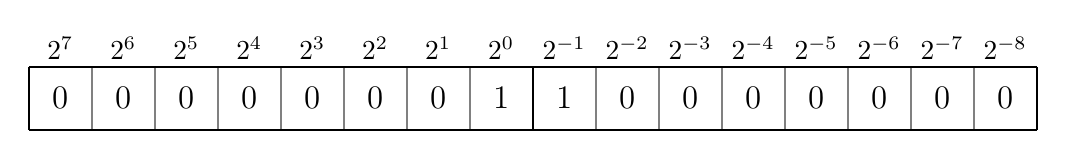
\begin{tikzpicture}[scale=0.8, every node/.style={scale=0.99}]


\colorlet{LighterMark}{black!50}

\foreach \i in {1,...,15}
{
     \draw[thick,LighterMark] (\i,1) -- (\i,0);
}

     \draw[thick,black] (0,1) -- (0,0);
      \draw[thick,black] (8,1) -- (8,0);
      \draw[thick,black] (16,1) -- (16,0);
      
\draw[thick,black] (0,0) -- (16,0);
\draw[thick,black] (0,1) -- (16,1);
 

%\foreach \i[evaluate={\pow=int(7-\i)}] in {0,...,7}
\foreach \i[evaluate={\pow=int(7-\i)}] in {0,...,7}
{
   \node[] at (\i+0.5,1.3){$2^{\pow}$  }  ;
      
         
     
}

%\foreach \i[evaluate={\pow=int((\i-7)*2)}]  in {8,...,15}
\foreach \i[evaluate={\pow=int(\i-7)}]  in {8,...,15}
{
     \node[] at (\i+0.5,1.3){$2^{-\pow}$}  ;
}

\tikzstyle{fontbf} = [font=\large]
\node[fontbf] at (0.5,0.5){0} ;
\node[fontbf] at (1.5,0.5){0};  
\node[fontbf] at (2.5,0.5){0} ; 
\node[fontbf] at (3.5,0.5){0} ;

\node[fontbf] at (4.5,0.5){0} ;
\node[fontbf] at (5.5,0.5){0};  
\node[fontbf] at (6.5,0.5){0} ; 
\node[fontbf] at (7.5,0.5){1} ;

\node[fontbf] at (8.5,0.5){1} ;
\node[fontbf] at (9.5,0.5){0};  
\node[fontbf] at (10.5,0.5){0} ; 
\node[fontbf] at (11.5,0.5){0} ;

\node[fontbf] at (12.5,0.5){0} ;
\node[fontbf] at (13.5,0.5){0};  
\node[fontbf] at (14.5,0.5){0} ; 
\node[fontbf] at (15.5,0.5){0} ;


\end{tikzpicture}

   \caption{* 1.5} 
\end{figure} 
\par
First shift both operators by 4 bits to the right:\\
\par
\begin{figure}[H]
 \centering
   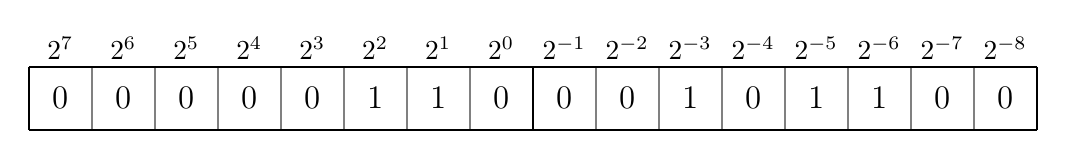
\begin{tikzpicture}[scale=0.8, every node/.style={scale=0.99}]


\colorlet{LighterMark}{black!50}

\foreach \i in {1,...,15}
{
     \draw[thick,LighterMark] (\i,1) -- (\i,0);
}

     \draw[thick,black] (0,1) -- (0,0);
      \draw[thick,black] (8,1) -- (8,0);
      \draw[thick,black] (16,1) -- (16,0);
      
\draw[thick,black] (0,0) -- (16,0);
\draw[thick,black] (0,1) -- (16,1);
 

%\foreach \i[evaluate={\pow=int(7-\i)}] in {0,...,7}
\foreach \i[evaluate={\pow=int(7-\i)}] in {0,...,7}
{
   \node[] at (\i+0.5,1.3){$2^{\pow}$  }  ;
      
         
     
}

%\foreach \i[evaluate={\pow=int((\i-7)*2)}]  in {8,...,15}
\foreach \i[evaluate={\pow=int(\i-7)}]  in {8,...,15}
{
     \node[] at (\i+0.5,1.3){$2^{-\pow}$}  ;
}

\tikzstyle{fontbf} = [font=\large]
\node[fontbf] at (0.5,0.5){0} ;
\node[fontbf] at (1.5,0.5){0};  
\node[fontbf] at (2.5,0.5){0} ; 
\node[fontbf] at (3.5,0.5){0} ;

\node[fontbf] at (4.5,0.5){0} ;
\node[fontbf] at (5.5,0.5){1};  
\node[fontbf] at (6.5,0.5){1} ; 
\node[fontbf] at (7.5,0.5){0} ;

\node[fontbf] at (8.5,0.5){0} ;
\node[fontbf] at (9.5,0.5){0};  
\node[fontbf] at (10.5,0.5){1} ; 
\node[fontbf] at (11.5,0.5){0} ;

\node[fontbf] at (12.5,0.5){1} ;
\node[fontbf] at (13.5,0.5){1};  
\node[fontbf] at (14.5,0.5){0} ; 
\node[fontbf] at (15.5,0.5){0} ;


\end{tikzpicture}

\end{figure} 
\par
\begin{figure}[H]
 \centering
   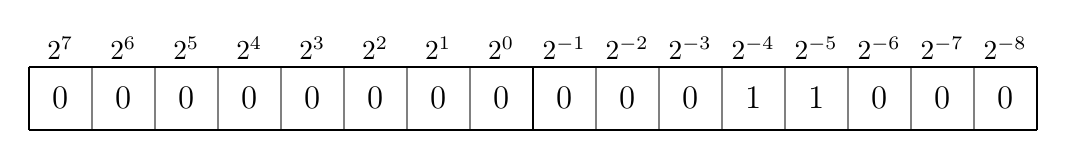
\begin{tikzpicture}[scale=0.8, every node/.style={scale=0.99}]


\colorlet{LighterMark}{black!50}

\foreach \i in {1,...,15}
{
     \draw[thick,LighterMark] (\i,1) -- (\i,0);
}

     \draw[thick,black] (0,1) -- (0,0);
      \draw[thick,black] (8,1) -- (8,0);
      \draw[thick,black] (16,1) -- (16,0);
      
\draw[thick,black] (0,0) -- (16,0);
\draw[thick,black] (0,1) -- (16,1);
 

%\foreach \i[evaluate={\pow=int(7-\i)}] in {0,...,7}
\foreach \i[evaluate={\pow=int(7-\i)}] in {0,...,7}
{
   \node[] at (\i+0.5,1.3){$2^{\pow}$  }  ;
      
         
     
}

%\foreach \i[evaluate={\pow=int((\i-7)*2)}]  in {8,...,15}
\foreach \i[evaluate={\pow=int(\i-7)}]  in {8,...,15}
{
     \node[] at (\i+0.5,1.3){$2^{-\pow}$}  ;
}

\tikzstyle{fontbf} = [font=\large]
\node[fontbf] at (0.5,0.5){0} ;
\node[fontbf] at (1.5,0.5){0};  
\node[fontbf] at (2.5,0.5){0} ; 
\node[fontbf] at (3.5,0.5){0} ;

\node[fontbf] at (4.5,0.5){0} ;
\node[fontbf] at (5.5,0.5){0};  
\node[fontbf] at (6.5,0.5){0} ; 
\node[fontbf] at (7.5,0.5){0} ;

\node[fontbf] at (8.5,0.5){0} ;
\node[fontbf] at (9.5,0.5){0};  
\node[fontbf] at (10.5,0.5){0} ; 
\node[fontbf] at (11.5,0.5){1} ;

\node[fontbf] at (12.5,0.5){1} ;
\node[fontbf] at (13.5,0.5){0};  
\node[fontbf] at (14.5,0.5){0} ; 
\node[fontbf] at (15.5,0.5){0} ;


\end{tikzpicture}

\end{figure} 
\par

Finally multiply them together:

\begin{figure}[H]
 \centering
   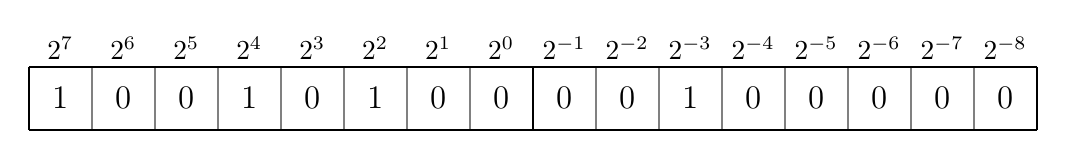
\begin{tikzpicture}[scale=0.8, every node/.style={scale=0.99}]


\colorlet{LighterMark}{black!50}

\foreach \i in {1,...,15}
{
     \draw[thick,LighterMark] (\i,1) -- (\i,0);
}

     \draw[thick,black] (0,1) -- (0,0);
      \draw[thick,black] (8,1) -- (8,0);
      \draw[thick,black] (16,1) -- (16,0);
      
\draw[thick,black] (0,0) -- (16,0);
\draw[thick,black] (0,1) -- (16,1);
 

%\foreach \i[evaluate={\pow=int(7-\i)}] in {0,...,7}
\foreach \i[evaluate={\pow=int(7-\i)}] in {0,...,7}
{
   \node[] at (\i+0.5,1.3){$2^{\pow}$  }  ;
      
         
     
}

%\foreach \i[evaluate={\pow=int((\i-7)*2)}]  in {8,...,15}
\foreach \i[evaluate={\pow=int(\i-7)}]  in {8,...,15}
{
     \node[] at (\i+0.5,1.3){$2^{-\pow}$}  ;
}

\tikzstyle{fontbf} = [font=\large]
\node[fontbf] at (0.5,0.5){1} ;
\node[fontbf] at (1.5,0.5){0};  
\node[fontbf] at (2.5,0.5){0} ; 
\node[fontbf] at (3.5,0.5){1} ;

\node[fontbf] at (4.5,0.5){0} ;
\node[fontbf] at (5.5,0.5){1};  
\node[fontbf] at (6.5,0.5){0} ; 
\node[fontbf] at (7.5,0.5){0} ;

\node[fontbf] at (8.5,0.5){0} ;
\node[fontbf] at (9.5,0.5){0};  
\node[fontbf] at (10.5,0.5){1} ; 
\node[fontbf] at (11.5,0.5){0} ;

\node[fontbf] at (12.5,0.5){0} ;
\node[fontbf] at (13.5,0.5){0};  
\node[fontbf] at (14.5,0.5){0} ; 
\node[fontbf] at (15.5,0.5){0} ;


\end{tikzpicture}

   \caption{148.125} 
\end{figure} 
$128 + 16 + 4 + 0.125 = 148.125 $\\
\par
Notice that you have to be careful. In the previous example some precision was lost ($ 2^{-8}$ bit disappeared during the $\gg 4$ operation) and an overflow could have occurred (multiplying by 3 instead of 1.5 would have gone past the precision of 8:8).\\
\par
In the source code, all fixed points variables are 32 bits wide and use a special \cw{typedef}.\\
\par
\begin{minipage}{\textwidth}
 \lstinputlisting[language=C]{code/fixed.c}
 \end{minipage}
\par
But not all \cw{fixed} are the same. Some are \cw{16:16}, some are \cw{24:8}. As a result some operations can be implemented differently. The multiplication for example can be either as follow.\\
\par
\begin{minipage}{\textwidth}
 \lstinputlisting[language=C]{code/fixed_mul.c}
 \end{minipage}
\par
Or it can be more complex due to a type of tweaked \cw{fixed} used for raycasting where the leftmost bit stores the sign via two's complement representation.\\
\par
\begin{minipage}{\textwidth}
 \lstinputlisting[language=C,morekeywords={asm,fixed}]{code/FixedByFrac.c}
 \end{minipage}
\par


 \textbf{\underline{Trivia :}}  Fixed Point Arithmetic usage was not limited to PC gaming. Many game console manufactured in the 90s and later featured no hardware floating point unit: Sony's original PlayStation (1994) and Sega's Saturn (1994) are examples among many with a design choice that not only reduced the production cost but also maximized the CPU pipeline throughput.
 

 
 


\subsubsection{Coordinate System}
With the CPU \cw{float}/\cw{int} problem out of the way, it is almost time to study how a ray is cast. The coordinate system finds its origin in the upper left. A map is a grid of 64 by 64 blocks. 
\begin{figure}[H]
  \centering
 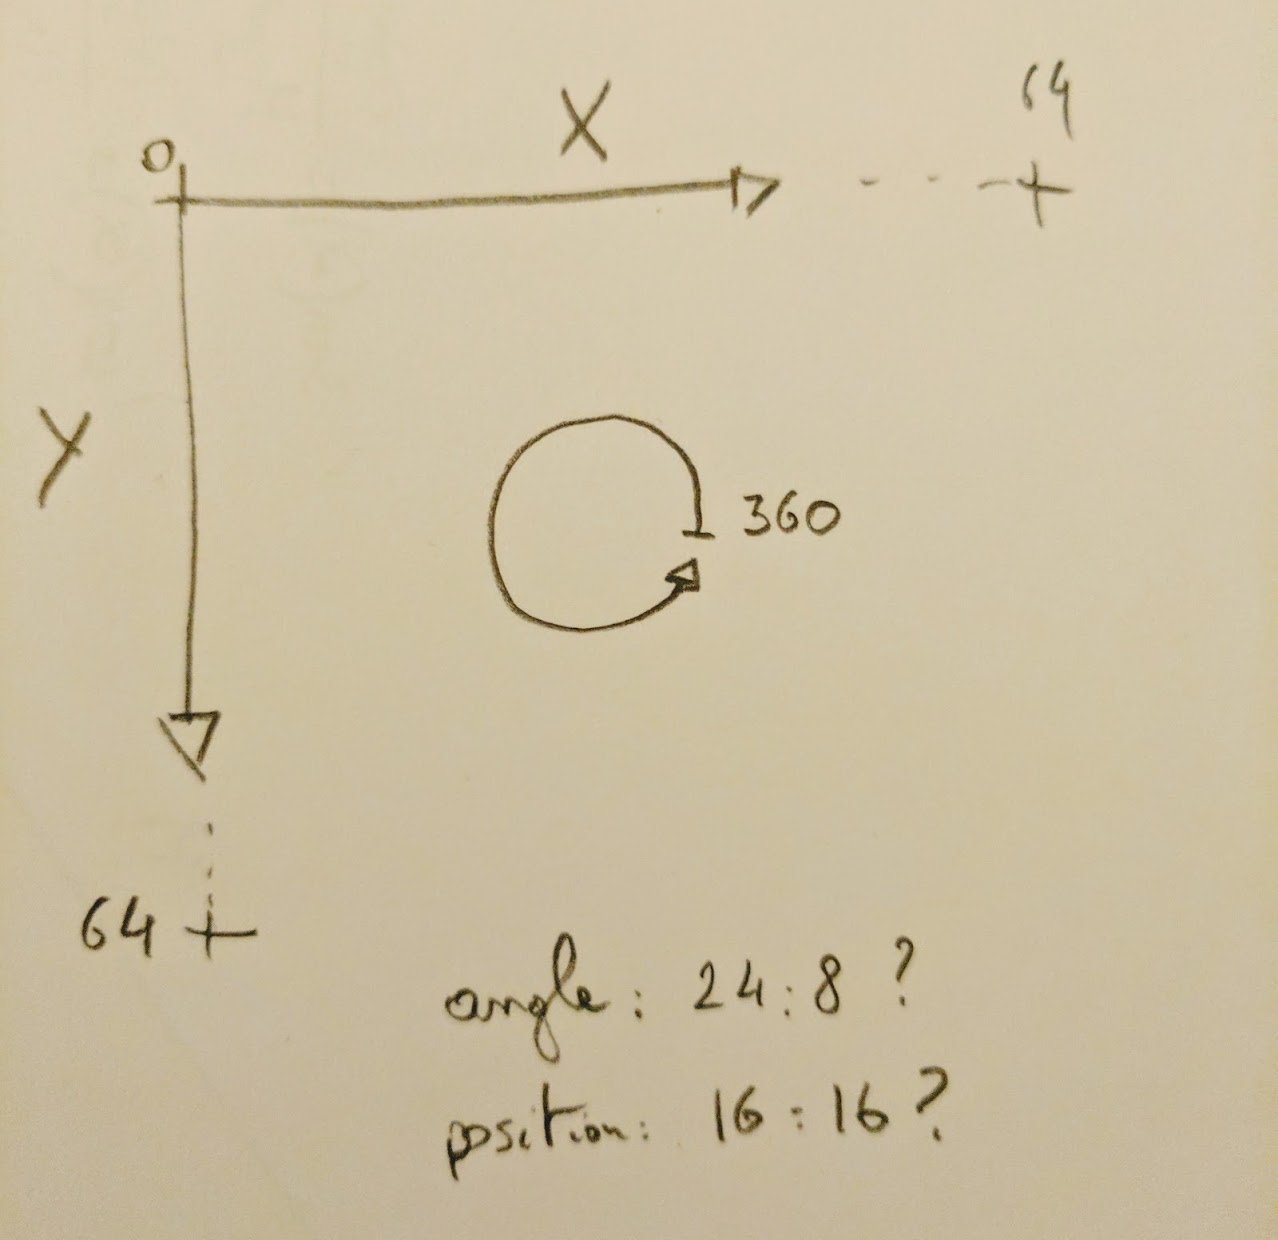
\includegraphics[width=.5\textwidth]{imgs/drawings/coordinate_system.png}
\end{figure}
\par
Since one block is 8 feet, maps can be 512 feet wide and tall. Fixed point variables are used all over the place. Column heights are 29:3. The player position is 16:16. Angles however are \cw{int}s representing 10th of degrees with a range [0, 3600].

















\subsubsection{Square World and RayCasting}
Drawing the walls is all about determining what is visible, what is not and what is in front of what. Michael Abrash's view on the topic tells it all:\\
\par
\begin{fancyquotes}
I want to talk about what is, in my book, the toughest 3-D problem of all, visible surface determination (drawing the proper surface at each pixel), and its close relative, culling (discarding non-visible polygons as quickly as possible, a way of accelerating visible surface determination). In the interests of brevity, I'll use the abbreviation VSD to mean both visible surface determination and culling from now on.
 \bigskip \\
Why do I think VSD is the toughest 3-D challenge? Although rasterization issues such as texture mapping are fascinating and important, they are tasks of relatively finite scope, and are being moved into hardware as 3-D accelerators appear; also, they only scale with increases in screen resolution, which are relatively modest.
 \bigskip \\
In contrast, VSD is an open-ended problem, and there are dozens of approaches currently in use. Even more significantly, the performance of VSD, done in an unsophisticated fashion, scales directly with scene complexity, which tends to increase as a square or cube function, so this very rapidly becomes the limiting factor in doing realistic worlds. I expect VSD increasingly to be the dominant issue in realtime PC 3-D over the next few years, as 3-D worlds become increasingly detailed.
 \bigskip \\
\textbf{Michael Abrash - Programmer}
 \end{fancyquotes}
 \par
VSD is not only complicated to get done, it is also hard to get done fast. It is easy to understand with a small example where objects are of free form with no alignment like in the following drawing.

\par
\begin{figure}[H]
\centering
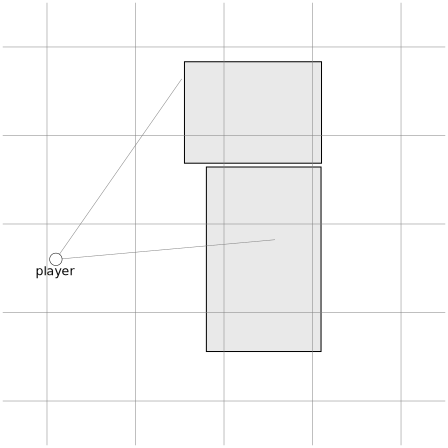
\includegraphics[width=\textwidth]{imgs/drawings/casting_a_ray/situation.pdf}
 
\end{figure}

In a world with no constraint, it is difficult to find the intersection of a ray with an object.\\
\par
In the example above, a valid approach would be to iterate over all objects in the world and perform ray marching which consist in checking a ray intersection with objects at a regular interval. But that is very CPU intensive and even with fixed point that would not be fast enough.
\begin{figure}[H]
\centering
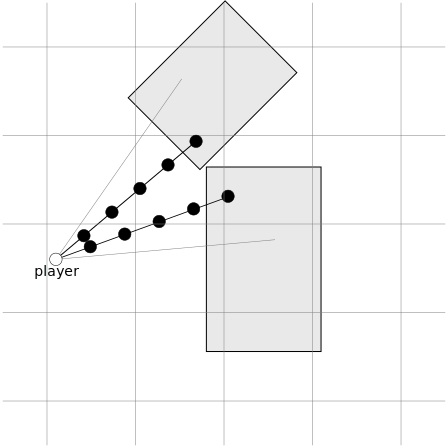
\includegraphics[width=\textwidth]{imgs/drawings/casting_a_ray/unaligned.pdf}
 \caption{Ray Marching in action.}
\end{figure}


In a world with some contraints the problem become much simpler. If a map is made of alixed aligned square block evenly distributed on a grid, the solution giving 100\% accuracy and low runtime overhead is to check for 'hits` only where a ray crosses the grid. This is the choice Wolfenstein 3D made and that explains why it can only draw perpendicular walls, all of them being 8 feet by 8 feet by 8 feet cubes.
\begin{figure}[H]
\centering
\includegraphics[width=\textwidth]{imgs/drawings/casting_a_ray/fixed.pdf}
 \caption{Blocks aligned with a grid.}
\end{figure}
\par
These constraints enable a variant of the DDA algorithm\footnote{Digital differential analyzer}, a fast and accurate way to detect where a ray hits a wall on the map.
\par
\begin{fancyquotes}
\par
Much was made about the "ray casting" used in Wolfenstein, but the real reason for it was that I had a lot of trouble with wall-span rendering in Catacombs 3D.  C3D (and Hovertank before that) shipped with various graphics glitches that you could get in some combinations of map block configurations, position, and viewing angle.  Some were due to fixed point precision issues not being handled optimally, and some were due to clipping and culling issues that I didn't really get a handle on until a couple years later.  In any case, they bothered me a lot.  Spurious graphics glitches do a lot of harm to the sense of immersion in a game, and I very much wanted Id games to feel "rock solid".
 \bigskip \\
There was a clear performance cost to it - doing 320 traces through a tile map and treating each column independently is much slower than looping through a few long wall segments.  However, the resulting code was small and very regular compared to the hairball of my wall span renderers, and it did deliver the rock-solid feel I wanted.
 \bigskip \\
If you made extremely jagged block maps that would turn into many dozen independent wall segments, the ray casting could start to look like a good performance choice, but few scenes were even close to that.  This is exactly the same ray tracing versus rasterization performance tradeoff that is still being made today, but now it is "how many tens of millions of triangles per frame to ray tracing break-even" instead of "how many dozen wall segments".
 \bigskip \\
\textbf{John Carmack - Programmer}
 \end{fancyquotes}



 \par
\begin{figure}[H]
  \centering
 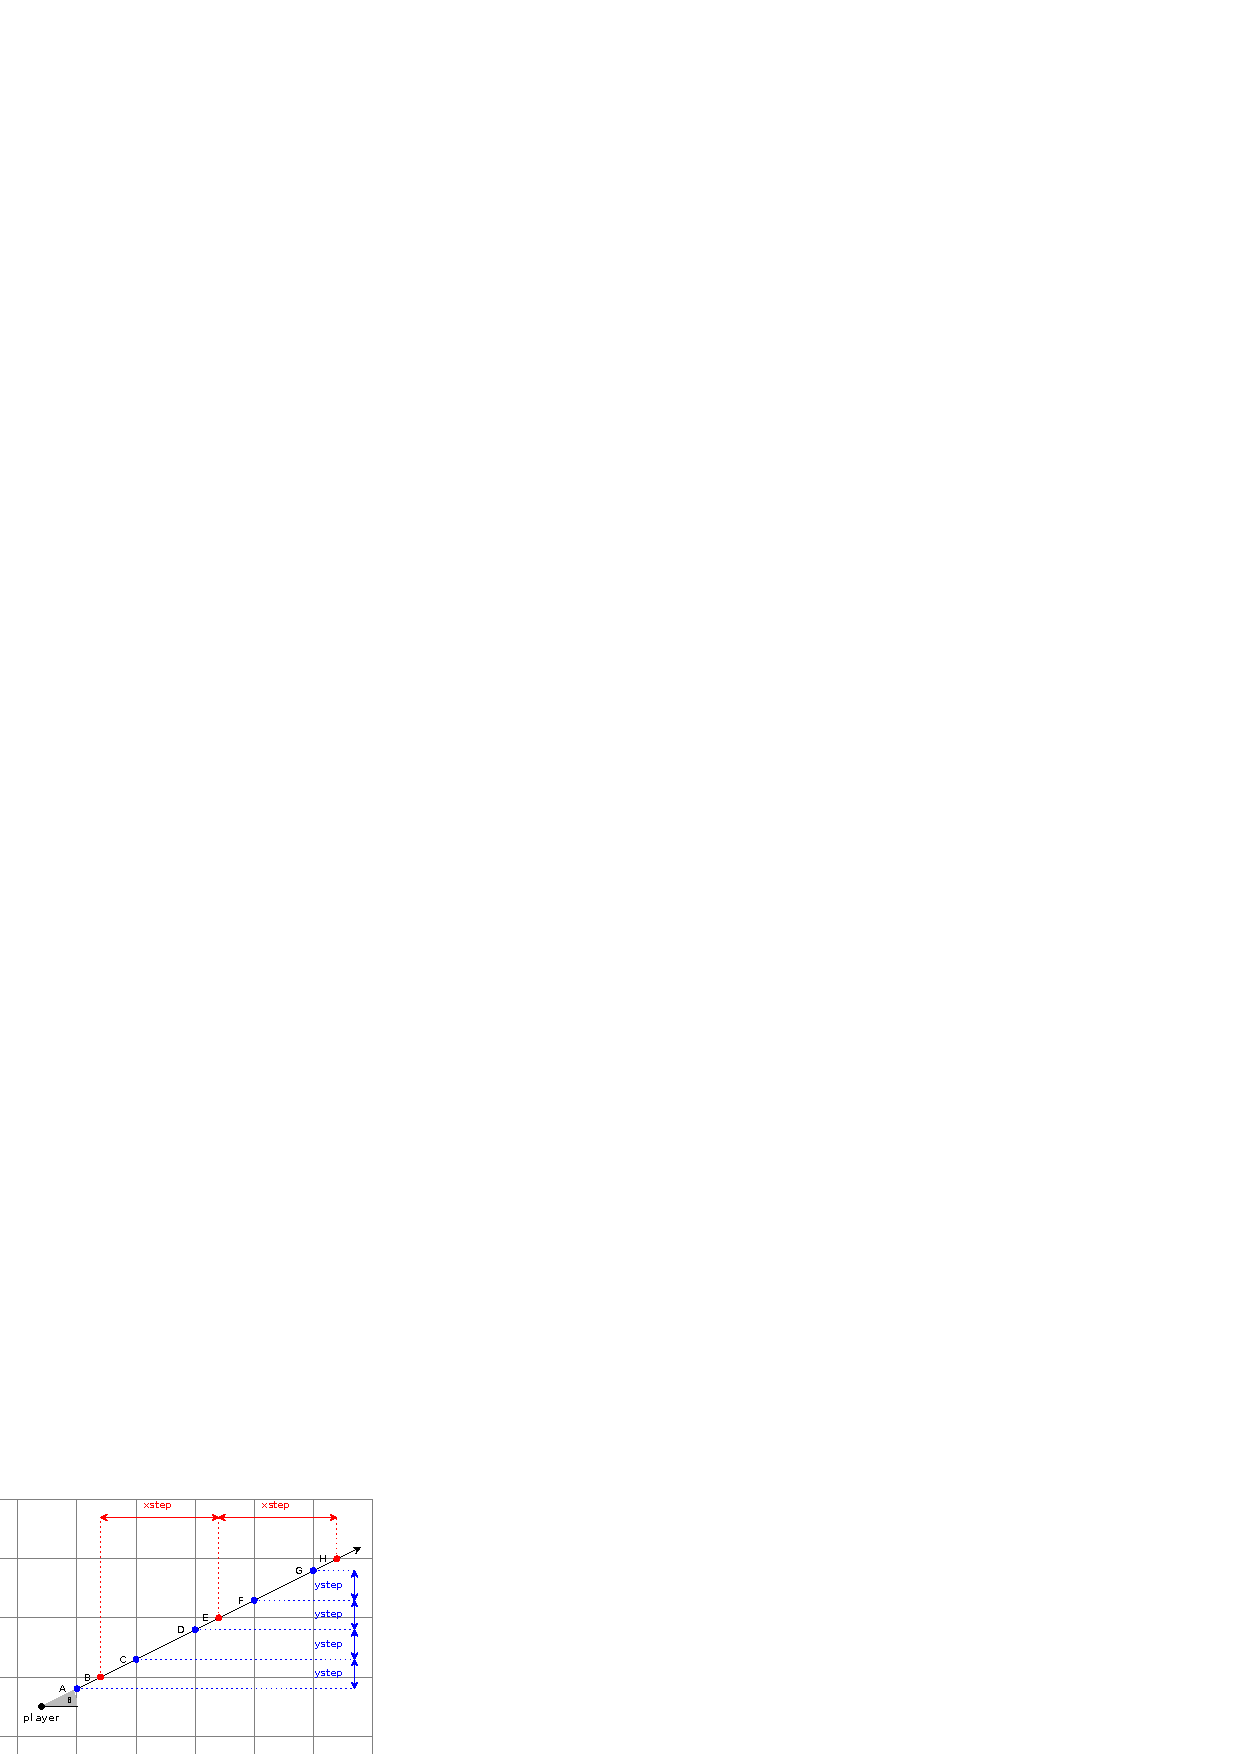
\includegraphics[width=\textwidth]{imgs/drawings/dda.pdf}
\end{figure}
\par
The reason DDA is so fast is because once the first intersection of a ray with an axis is known (A for Y axis and B for X axis) all subsequent intersections coordinate are two cheap additions away.
\par


\begin{equation*}
    \scalebox{1.3}{
$C = (A.x +1, A.y + xstep)$\\
}
\end{equation*}
\begin{equation*}
    \scalebox{1.3}{
$D = (C.x +1, C.y + xstep)$\\
}
\end{equation*}
\begin{equation*}
    \scalebox{1.3}{
$F = (D.x +1, D.y + xstep)$\\
}
\end{equation*}
\begin{equation*}
    \scalebox{1.3}{
$G = (F.x +1, F.y + xstep)$\\
}
\end{equation*}


\par
In a similar fashion for the vertical intersections:\\
  \begin{equation*}
    \scalebox{1.3}{

$E = (B.x + ystep, A.y + 1)$\\
}
\end{equation*}
  \begin{equation*}
    \scalebox{1.3}{
$D = (E.x + ystep, E.y + 1)$\\
}
\end{equation*}
Note that $ystep$ and $ystep$ are simple lookup into the \cw{tan} array since $xstep=tan(\theta)$ and $ystep=(90-\theta)$ where $\theta$ is the angle of the ray in map coordinates. This CPU power limitation and associated grid solution bubbled up all the way to the game designer. It explains why all Wolfenstein 3D maps are made of axis aligned square elements.\\
\par
\begin{figure}[H]
  \centering
 \fullimage{e1m1.png}
 \caption{The legendary E1M1. Player is the green arrow at the bottom.}
\end{figure}


\subsubsection{Call Apogee}
With map being simple and fast to draw, a contest was to be held. Find a special item in a particularly difficult to access place in the game and call the publisher (Apogee). The maze is located in Episode 2, Map 8.\\
\par
\begin{figure}[H]
  \centering
 \fullimage{e2m8.png}
 \caption{E2M8}
\end{figure}

\par

\begin{minipage}{.5\textwidth}
Behind a forest of push walls (white squares) and angry bosses (blue circles), a sign finally showed up (the red triangle). \\
\par 
However due to people reverse engineering the map format and cheat sites allowing players to find the maze, the sign was replaced with a skeleton with all game shipping during 1992.\\ In the previous map notice there are no push wall leading to the red triangle, the room is hidden.\\
 \end{minipage}
\begin{minipage}{.5\textwidth}
\begin{figure}[H]
 \centering
 \scaledimage{0.9}{call_apogee.png} 
\end{figure}
\end{minipage}

\par
\begin{fancyquotes}
"Call Apogee and say Aardwolf."  It's a sign that to this day is something
that I get asked about a lot.  This is a sign that appears on a wall in a
particularly nasty maze in Episode 2 Level 8 of Wolfenstein 3D.  The sign
was to be the goal in a contest Apogee was going to have, but almost
immediately after the game's release, a large amount of cheat and mapping
programs were released.  With these programs running around, we felt that
it would have been unfair to have the contest and award a prize.  The sign
was still left in the game, but in hindsight, probably should have been
taken out.  To this day, Apogee gets letters and phone calls and asking
what Aardwolf is, frequently with the question, "Has anyone seen this yet?"\\
\\
Also, in a somewhat related issue, letters were shown after the highest score
in the score table in some revisions of the game.  These letters were to be
part of another contest that got scrapped before it got started, where we were
going to have people call in with their scores and tell us the code; we'd then
be able to verify their score.  However, with the cheat programs out there,
this got scrapped too.\\
\\
Basically, "Aardwolf" and the letters mean nothing now.  Also note that if
you found the Aardwolf sign in the game (without cheating), there's a VERY
strong chance that you're stuck in there.  The only way out may be to restart,
or load a saved game from before you went into that maze.\\
\\
\textbf{Joe Siegler - Past Pioneers of the Shareware Revolution}
\end{fancyquotes}
\par
\bu{Trivia :} What is Aardwolf? A maned striped mammal (Proteles cristatus) of southern and eastern Africa that resembles the related hyenas and feeds chiefly on carrion and insects. It was back then the mascot of Id, appearing on Tom's Gotta Lists and the Commander Keen 6 Hint Sheet.














 
 
 
 
 
 
 
 
\subsubsection{Raycasting: DDA Algorithm}
The DDA intersection algorithm is implemented in a fully handcrafted 740 lines of assembly routine: \cw{AsmRefresh}. It is represented here in pseudo-C for readability. It consists of two while loops (one each for vertical and horizontal intersections) ping-ponging with each other via goto. It is highly unorthodox and super efficient.\\
\par



\begin{minipage}{\textwidth}
\lstinputlisting[language=C]{code/flipflop.c}
\end{minipage}
This implementation results in many \cw{jmp} instructions. These would kill the i-cache and empty the pipeline on a modern CPU. But on a an architecture devoid of pipeline and code cache such as the 386 it is not a problem at all.\\
\par
This part of the code relies heavily on unit circle principles. Because we need to know by how much we go up/down when advancing on the X axis and how much we go left/right when advancing on the Y axis, the \cw{tan} function is expecially useful. It is easier to understand with the unit circle drawn (remember the circle radius R is equal to 1).
\begin{figure}[H]
\centering
 % \documentclass[crop,tikz,ifthenelse]{standalone}

% \usetikzlibrary{calc}
% \usepackage{tkz-euclide}
% \usetkzobj{all}


% \begin{document}
\begin{tikzpicture}[scale=2]

\coordinate(origin) at (0,0);
\coordinate(yaxis) at (0,6.5);
\coordinate(xaxis) at (6,0) ;

\draw (0,0) circle (2);
\draw[->,>= latex] (-2.4,0) -- (2.4,0);
\draw[->,>= latex] (0, -2.4) -- (0, 2.4);

// tangent line
\coordinate (tantop) at (2,2.4);
\coordinate (tanbottom) at (2,-2.4);
\draw[->,>= latex] (tanbottom) -- (tantop);

\coordinate (point) at (35:2);
\coordinate (origin) at (0,0);



\node[below left] {\Large $(0,0)$};

\coordinate (procsin) at ($(origin)!(point)!(yaxis)$);
\coordinate (projcos) at ($(origin)!(point)!(xaxis)$) ;

\node[left]  at (procsin) {\Large $sin(\theta)$};
\node[below] at (projcos) {\Large $cos(\theta)$};

\draw[dotted] (projcos) -- (point) ;
\draw[dotted] (procsin) -- (point) ;



\coordinate (extended_point) at (2,1.4);%(35:3);
%\coordinate (tan_point) at (intersection of origin--extended_point and tanbottom -- tantop );

\node[right] at (extended_point) {\Large $tan(\theta)$};

\tkzMarkAngle[fill= gray,size=0.6](xaxis,origin,extended_point);
\tkzLabelAngle[pos = 0.4](extended_point,origin,xaxis){\Large $\theta$};
\draw (origin) -- (extended_point) ;
\end{tikzpicture}
% \end{document}

\end{figure}
\par
When advancing 1 on the X axis, the ray moves up $tan(\alpha)$ on the Y axis. The reciprocal is calculated as follow: Move 1 on Y axis, move $tan(90-\alpha)$ on X axis. To accelerate \cw{cos}, \cw{sin} and \cw{tan} calculations, the engine uses lookup table. One entry for each 360 degres (read about lookup table trick in details in the "Tricks" section).




















\subsubsection{High school math}
Before proceeding to the next session describing what is done with the distance from the player to the wall, here is a short reminder of something taught in highschool, the fundation of most calculations in the engine: SOH-CAH-TOA.\\
\par
 \begin{fancyquotes}
  I'm no super mathematician-- I learned high school math well enough to solve real world problems with it.\\
 \par
\textbf{John Carmack - Programmer}
 \end{fancyquotes}


\par
\begin{figure}[H]
\centering
 % \documentclass{standalone}% 'crop' is the default for v1.0, before it was 'preview'
% \usepackage[x11names,dvipsnames]{xcolor} %Colocação de cores
% \usepackage{tikz,tikz-3dplot} %Para fazer desenhos
% \usepackage{tkz-euclide}
% \usetkzobj{all}
\begin{tikzpicture}[scale=1.5]

% \begin{document}
% \begin{tikzpicture}[]

\coordinate(A) at (0,0);
\coordinate(B) at (7,0);
\coordinate(C) at (0,5);

\draw[draw=black] (A) -- node[below] {\Large A} (B);
\draw[draw=black] (B) -- node[above] {\Large H} (C);
\draw[draw=black] (C) -- node[left] {\Large O} (A);

\tkzMarkRightAngle(B,A,C);
\tkzLabelAngle[pos = 1.0](A,B,C){\Large $\alpha$}
\tkzMarkAngle[fill= gray,size=1.8cm,opacity=.2](C,B,A)

\node (A) at (7.5,3.5) {\Large $sin(\alpha) = \frac{O}{H}$};
\node (A) at (7.5,2.5) {\Large $cos(\alpha) = \frac{A}{H}$};
\node (A) at (7.5,1.5) {\Large $tan(\alpha) = \frac{O}{A}$};

\end{tikzpicture}
%\end{document}
\end{figure}



This drawing is all the math you need to understand fish eye correction and coordinate projections used to place player, enemies, items and calculate sounds locations.\\






\subsubsection{Calculating column heights}
Once the intersection between a ray and a wall is found from coordinate (\cw{viewx},\cw{viewy}) to (\cw{xintercept},\cw{yintercept}), it is time to calculate how tall the column of pixel for this ray should be. It happens in the function \cw{CalcHeight}.\\

\begin{minipage}{\textwidth}
\lstinputlisting[language=C]{code/CalcHeight.c}
\end{minipage}

The code is not what one would expect. The raycasting algorithm is supposed to cast a ray for each pixel column and use the distance \codeword{d} to infer the column's height on screen. So it would have made sense to see a formula like:
\begin{figure}[H]
  \centering
  \begin{equation*}
    \scalebox{1.3}{
$ d = \sqrt{dx^2 + dy^2}$ 
 }
  \end{equation*}
\end{figure}
But instead the code looks like it is doing: 
\begin{figure}[H]
  \centering
  \begin{equation*}
    \scalebox{1.3}{
$d = dx * \cos(\alpha) - dy * \sin(\alpha) $
 }
  \end{equation*}
\end{figure}
Something is fishy here. Let's explain with an example.\\
\par
\begin{figure}[H]
\centering
 %\documentclass[tikz,border=2pt,png]{standalone}
%\usepackage{tkz-euclide}
%\usetkzobj{all}
%\begin{document}
\begin{tikzpicture}[scale=2.0]

\coordinate(origin) at (0,0)[label=below:view] {};
\coordinate(yaxis) at (0,6.5){};
\coordinate(xaxis) at (6,0) {};
\coordinate(angle) at (30:3);
\coordinate(intercept) at (3,5) {};

\node[below left] (orign) {viewpoint};
\node[below right] (_XX) at (intercept) {intercept};

% AXIS
%\draw[->,draw=black,>=stealth] (origin)  -- (xaxis) ;
%\draw[->,draw=black,>=stealth] (origin)  -- (yaxis) ;
%\draw[draw=black] (origin)  -- (0,-0.5) ;
%\draw[draw=black] (origin)  -- (-0.5,0) ;

% WALL
\fill[black!20!white, draw=black] (2,5) rectangle (4,7);
%\fill[black!20!white, draw=black] (4,5) rectangle (6,7);
%\fill[black!20!white, draw=black] (4,3) rectangle (6,5);


\fill (intercept) circle (2pt);


\draw[->,draw=gray,>=stealth] (origin)  -- (angle) ;

\coordinate (dx) at ($(origin)!(intercept)!(xaxis)$);
\draw[draw=gray,>=stealth,dashed] (origin) -- node[below] {dx} (dx);
\draw[draw=gray,>=stealth,dashed] (intercept) -- node[right] {dy}(dx);

\tkzMarkAngle[fill= gray,size=0.8cm,opacity=.2](xaxis,origin,angle)
\tkzLabelAngle[pos = 0.6](xaxis,origin,angle){$\alpha$}

\fill[fill=black] (origin) circle (2pt);

\draw[] (origin) -- node[below] {d} ++(intercept) ;

%\draw[] 


\end{tikzpicture}
%\end{document}
 \caption{Raycasting using distance d} \label{fig:Raycasting2}
\end{figure}

In this drawing the player is located at \cw{viewpoint} with a view angle \begin{math}\alpha\end{math}. A ray has been cast from \cw{viewpoint} and it hit a wall at \cw{intercept}. The distance \codeword{d} is a straight line between the player point of view and the location where the ray hit the line which can be obtained with $d = \sqrt{dx^2 + dy^2}$. Repeated for all rays, such an algorithm would result in a "fisheye effect".









\begin{minipage}{\textwidth}

    \begin{figure}[H]
    \centering
      \fullimage{fish_eye/bad_mild.png}
     \caption{Fish eye effect: Mild}. \label{fig:mips}
     \end{figure} 


    \begin{minipage}{.4\textwidth}
    This visual artifact happens because the straight distance from the player to the wall is not constant. Walls are further away on the side of the screen and therefore represented smaller.\\
    To demonstrate the fish eye distortion, here are three screenshots from a modified version of the engine. It was altered to use distance \cw{d} instead of "something else" to calculate column heights. At first from a distance of 32 feet, the distorsion is barely noticeable.\\
     \end{minipage}
    \begin{minipage}{.6\textwidth}
    \begin{figure}[H]
      \begin{flushright}
     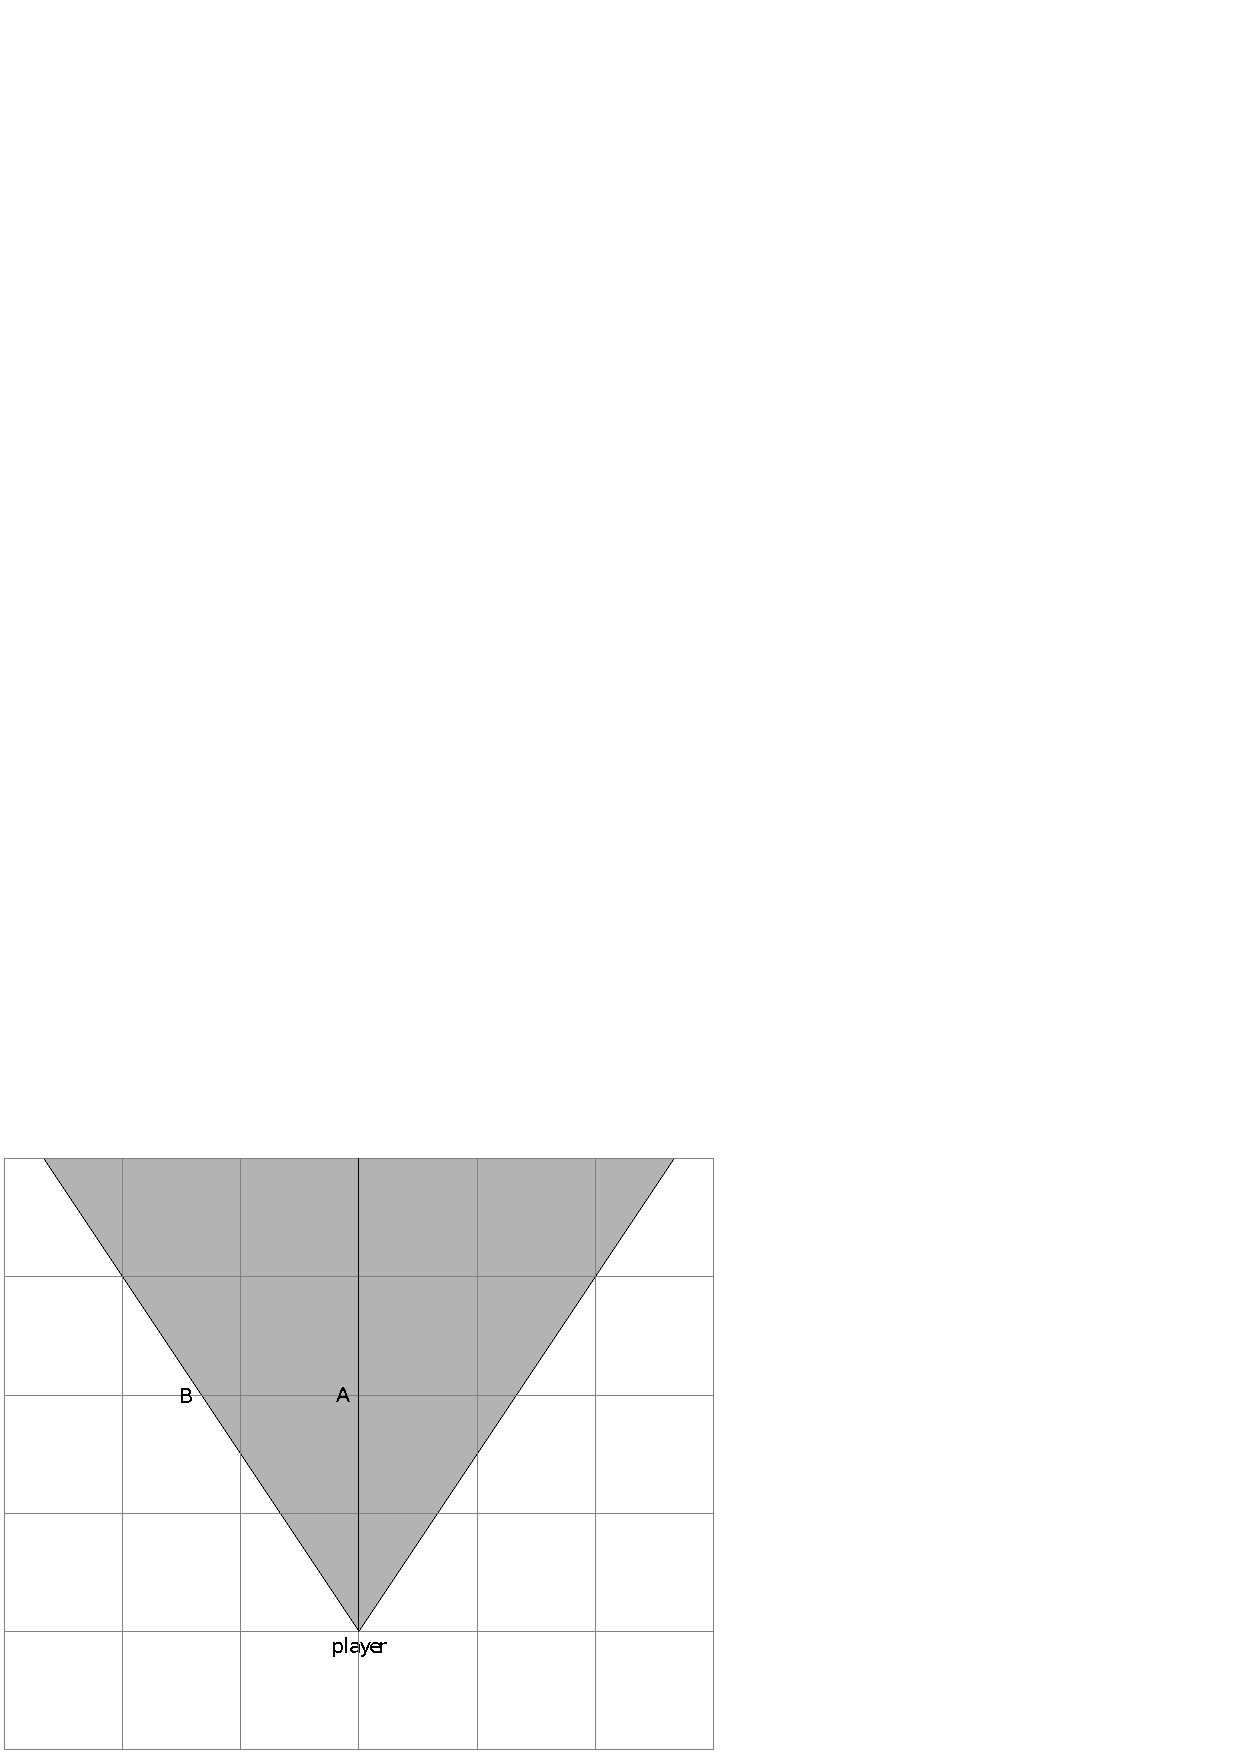
\includegraphics[width=.9\textwidth]{imgs/drawings/fish_eye/top_view_far.pdf}
       \end{flushright}
    \end{figure}
    \end{minipage}
\end{minipage}
\par



\begin{minipage}{\textwidth}
\begin{figure}[H]
\centering
  \fullimage{fish_eye/bad_ok.png}
 \caption{Fish eye effect: Bad} \label{fig:mips}
 \end{figure}
\begin{minipage}{.4\textwidth}
From a distance of 24 feet, the distortion cannot be ignored any more and the problem is clearly noticeable.\\
\par
Note that even though the player is getting closer to the wall, the ratio of A to B remain the same. Only the absolute difference in pixels height when the column is rendered on screen is increasing.
 \end{minipage}
\begin{minipage}{.6\textwidth}
\begin{figure}[H]
  \begin{flushright}
 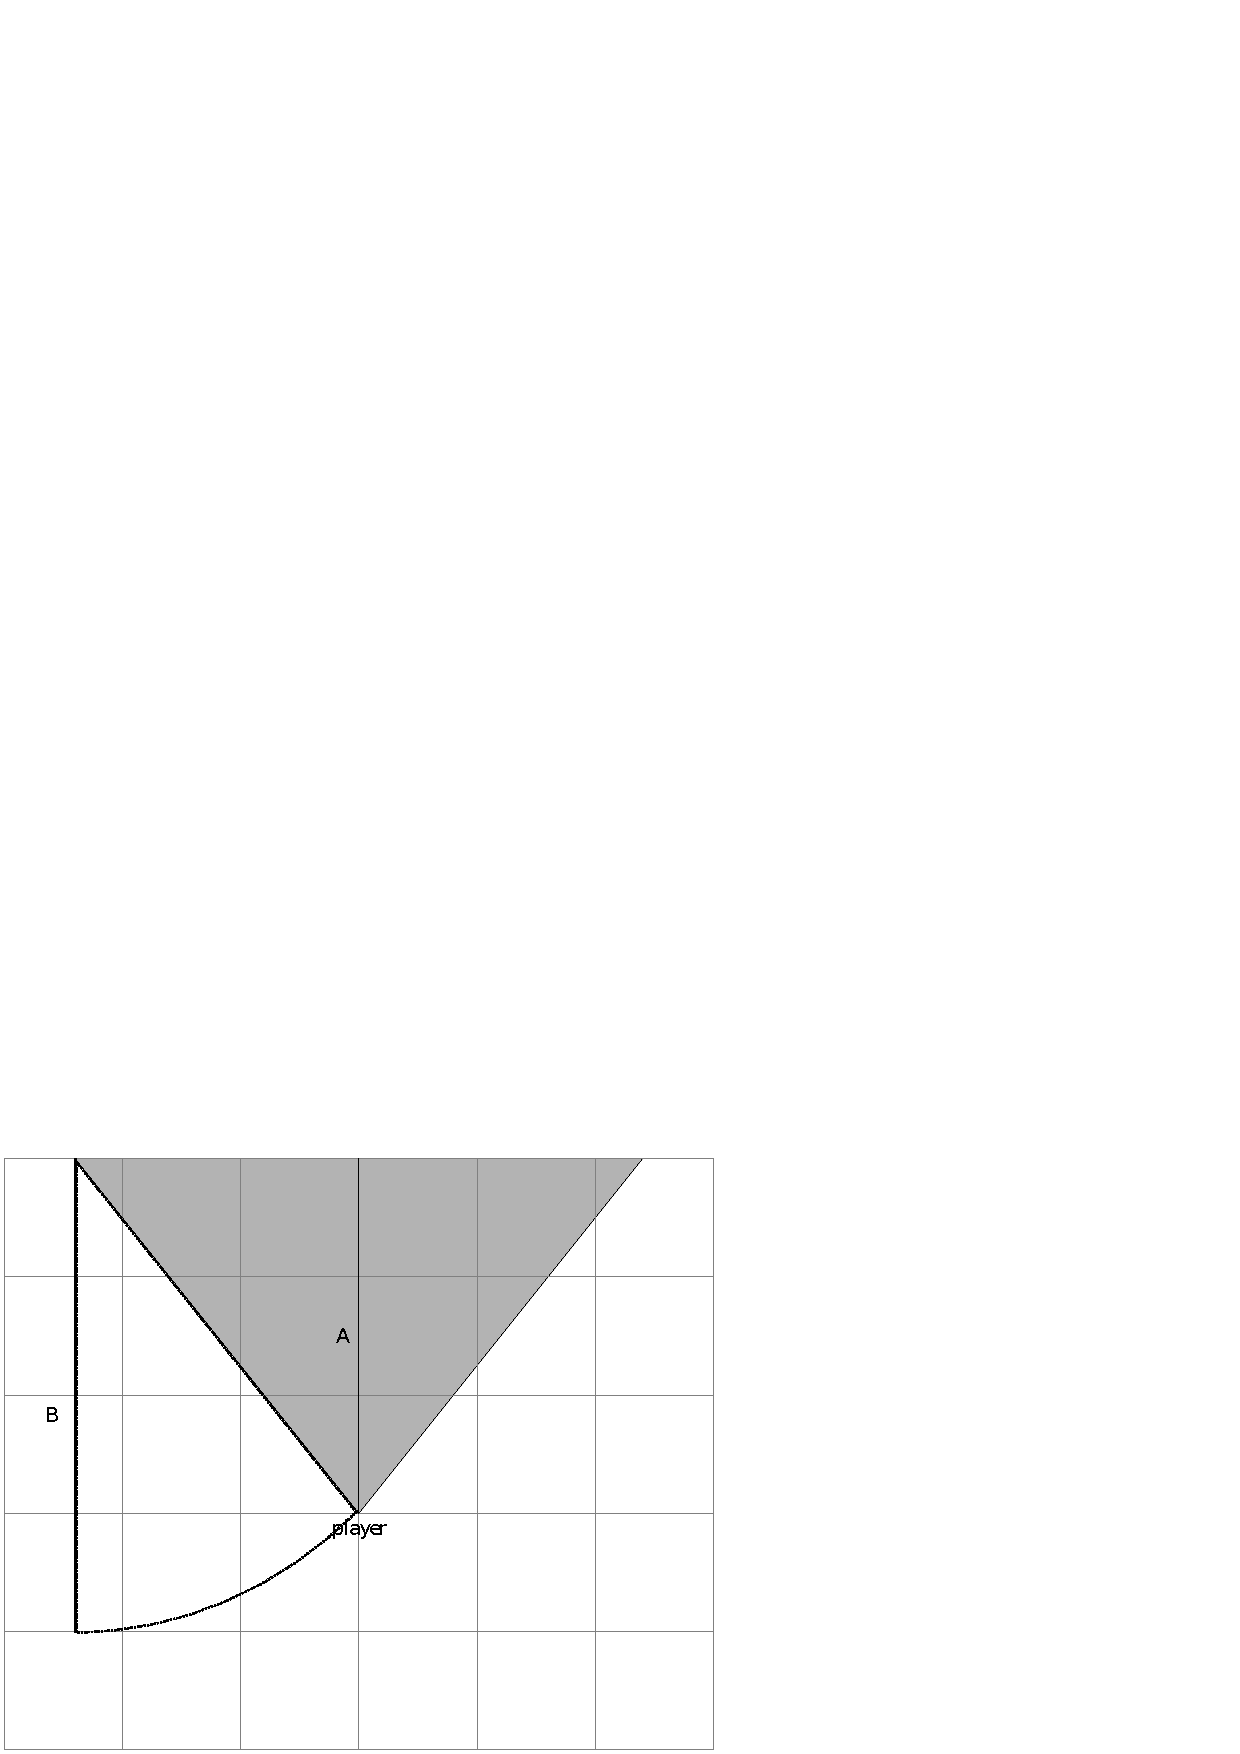
\includegraphics[width=.9\textwidth]{imgs/drawings/fish_eye/top_view_middle.pdf}
 \end{flushright}
\end{figure}
\end{minipage}
\end{minipage}




\begin{minipage}{\textwidth}
 \begin{figure}[H]
\centering
  \fullimage{fish_eye/bad_bad.png}
 \caption{Fish eye effect: AAAAARG} \label{fig:mips}
 \end{figure}
 

\begin{minipage}{.4\textwidth}
At a closer range (12 feet) the distortion is straight up unpleasant with a claustrophobic touch.\\
\par
To avoid this distortion and get a more pleasant rendition, what must be used is not the direct distance \cw{d} but \cw{d} projected on the camera plane (perpendicular to the view direction (\cw{z})).
 \end{minipage}
\begin{minipage}{.6\textwidth}
 \begin{figure}[H]
  \begin{flushright}
  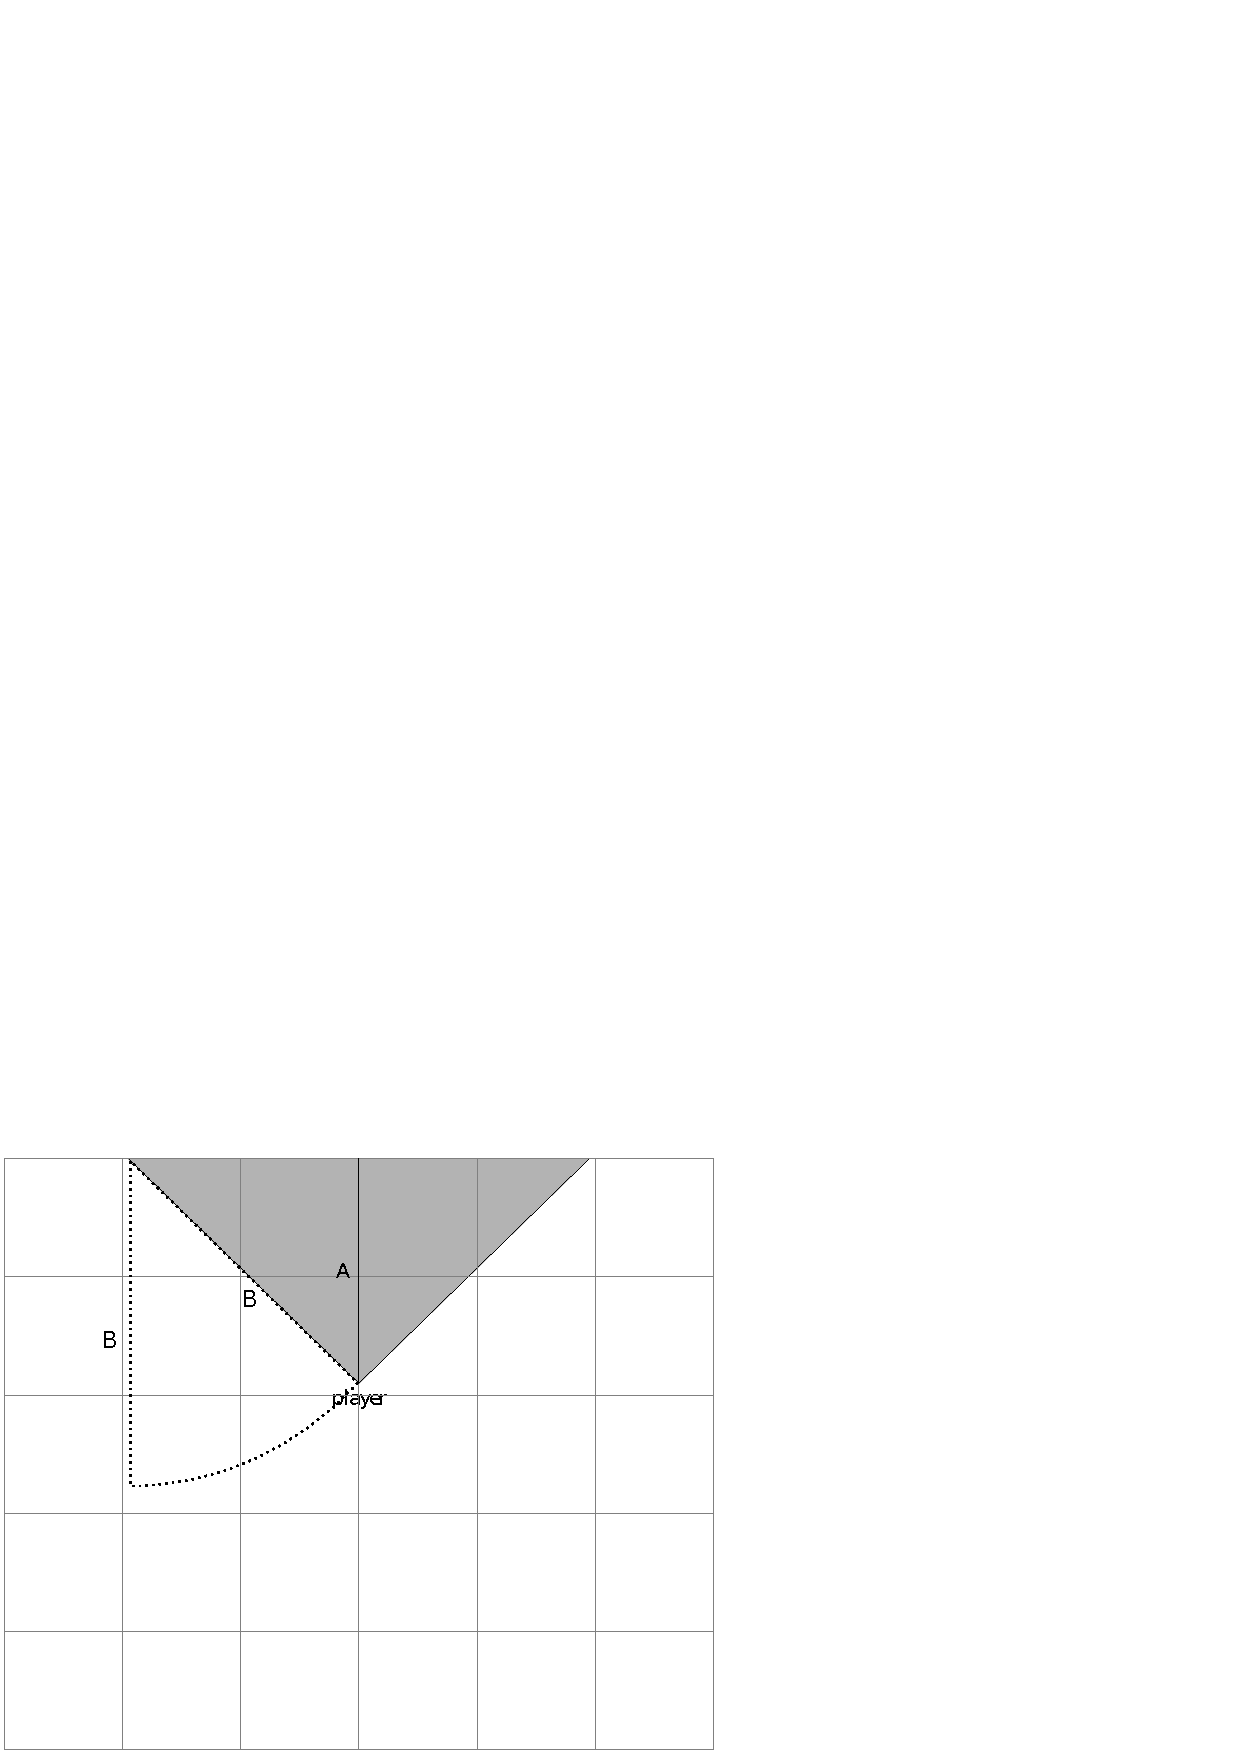
\includegraphics[width=.9\textwidth]{imgs/drawings/fish_eye/top_view_close.pdf}
 \end{flushright}
\end{figure}
 \end{minipage}
\end{minipage}
\par



\begin{figure}[H]

 %\documentclass[tikz,border=2pt,png]{standalone}
%\usepackage{tkz-euclide}
%\usetkzobj{all}
%\begin{document}
\begin{tikzpicture}[scale=2.0]

\coordinate(origin) at (0,0)[label=below:view] {};
\coordinate(yaxis) at (0,6.5){};
\coordinate(xaxis) at (6,0) {};
\coordinate(angle) at (30:3);
\coordinate(intercept) at (3,5) {};

\node[below left] (orign) {viewpoint};
\node[below right] (_XX) at (intercept) {intercept};

% plan
\coordinate(planA) at (120:5);
\coordinate(planB) at (-60:1);
\draw[draw=gray,dashed] (planA) -- (planB);
% AXIS
%\draw[->,draw=black,>=stealth] (origin)  -- (xaxis) ;
%\draw[->,draw=black,>=stealth] (origin)  -- (yaxis) ;
%\draw[draw=black] (origin)  -- (0,-0.5) ;
%\draw[draw=black] (origin)  -- (-0.5,0) ;

% WALL
\fill[black!20!white, draw=black] (2,5) rectangle (4,7);
%\fill[black!20!white, draw=black] (4,5) rectangle (6,7);
%\fill[black!20!white, draw=black] (4,3) rectangle (6,5);

% projected intercept
\coordinate (proj_intercept) at ($(planA)!(intercept)!(planB)$);
\draw[draw=black] (proj_intercept) -- node[above] {z} (intercept);

\tkzMarkRightAngle(intercept,proj_intercept,origin);
\tkzMarkRightAngle(angle,origin,proj_intercept);

\fill (intercept) circle (2pt);

% Angle
\draw[->,draw=gray,>=stealth] (origin)  -- (angle) ;

\coordinate (dx) at ($(origin)!(intercept)!(xaxis)$);
% DX and DY
\draw[draw=gray,>=stealth,dashed] (origin) -- node[below] {dx} (dx);
\draw[draw=gray,>=stealth,dashed] (intercept) -- node[right] {dy}(dx);

\tkzMarkAngle[fill= gray,size=0.8cm,opacity=.2](xaxis,origin,angle)
\tkzLabelAngle[pos = 0.6](xaxis,origin,angle){$\alpha$}

\fill[fill=black] (origin) circle (2pt);

% D libe
\draw[] (origin) -- node[below] {d} ++(intercept) ;

%\draw[] 


\end{tikzpicture}
%\end{document}
\label{fig:Raycasting2}
 
\end{figure}

This projection (z) is mathematically hard to calculate in one go (especially with fixed point). The trick is to break it down in two components and use the mnemonic SOH-CAH-TOA.\\


\begin{figure}[H]
\centering
 %\documentclass[tikz,border=2pt,png]{standalone}
%\usepackage{tkz-euclide}
%\usetkzobj{all}
%\begin{document}
\begin{tikzpicture}[scale=2.0]

\coordinate(origin) at (0,0)[label=below:view] {};
\coordinate(yaxis) at (0,6.5){};
\coordinate(xaxis) at (6,0) {};
\coordinate(angle) at (30:3);
\coordinate(intercept) at (3,5) {};

\node[below left] (orign) {viewpoint};
\node[below right] (_XX) at (intercept) {intercept};

% plan
\coordinate(planA) at (120:5);
\coordinate(planB) at (-60:1);
\draw[draw=gray,dashed] (planA) -- (planB);
% AXIS
%\draw[->,draw=black,>=stealth] (origin)  -- (xaxis) ;
%\draw[->,draw=black,>=stealth] (origin)  -- (yaxis) ;
%\draw[draw=black] (origin)  -- (0,-0.5) ;
%\draw[draw=black] (origin)  -- (-0.5,0) ;

% WALL
\fill[black!20!white, draw=black] (2,5) rectangle (4,7);
%\fill[black!20!white, draw=black] (4,5) rectangle (6,7);
%\fill[black!20!white, draw=black] (4,3) rectangle (6,5);

% projected intercept
\coordinate (proj_intercept) at ($(planA)!(intercept)!(planB)$);
\draw[draw=gray,dashed] (proj_intercept) -- node[above] {} (intercept);

\tkzMarkRightAngle[draw=gray](intercept,proj_intercept,origin);
\tkzMarkRightAngle[draw=gray](angle,origin,proj_intercept);

\fill (intercept) circle (2pt);

% Angle
%\draw[->,draw=gray,>=stealth] (origin)  -- (angle) ;

\coordinate (dx) at ($(origin)!(intercept)!(xaxis)$);
% DX and DY
\draw[draw=gray,>=stealth,dashed] (origin) -- node[below] {dx} (dx);
\draw[draw=gray,>=stealth,dashed] (intercept) -- node[right] {dy}(dx);

\tkzMarkAngle[fill= gray,size=0.8cm,opacity=.2](xaxis,origin,angle)
\tkzLabelAngle[pos = 0.6](xaxis,origin,angle){$\alpha$}

\fill[fill=black] (origin) circle (2pt);

\coordinate (A) at ($(origin)!(dx)!(angle)$);
\draw[] (origin)  -- node[below] {A} (A) ;

\coordinate (B) at ($(proj_intercept)!(dx)!(intercept)$);
\draw[] (intercept)  -- node[above] {B} (B) ;

\draw[draw=gray,dashed] (dx) -- (B) ;

\fill (A) circle (2pt);
\fill (B) circle (2pt);

\tkzMarkAngle[fill= gray,size=0.8cm,opacity=.2](intercept,dx,A)
\tkzLabelAngle[pos = 0.6](intercept,dx,A){$\alpha$}

\end{tikzpicture}
%\end{document}
 
\end{figure}
Using CAH gives $A = dx * \cos(\alpha)$ and SOH gives $B = dy * \sin(\alpha) $.\\
\par

Adding them together becomes:
\par
\begin{figure}[H]
  \centering
  \begin{equation*}
    \scalebox{1.3}{
$z = A + B = dx * \cos(\alpha) + dy * \sin(\alpha) $. 
 }
  \end{equation*}
\end{figure}
Since dx and dy are not distances but vectors (with a sign) the equation becomes: 


\begin{figure}[H]
  \centering
  \begin{equation*}
    \scalebox{1.3}{
$z = A + B = dx * \cos(-\alpha) + dy * \sin(-\alpha) $ 
 }
  \end{equation*}
\end{figure}
which simplified becomes: 

\begin{figure}[H]
  \centering
  \begin{equation*}
    \scalebox{1.3}{
$z = A + B = dx * \cos(\alpha) - dy * \sin(\alpha) $
 }
  \end{equation*}
\end{figure}
\par
For people who like equations, the overall operation can be seen as the multiplication of a rotation matrix with the vector intercept (dx,dy). It would rotate coordinates from map space to player space (where axis orientation is dictated by the player view angle).
\begin{figure}[H]
  \centering
  \begin{equation*}
    \scalebox{1.3}{
    $
      \begin{bmatrix} 
        \cos(\alpha) & -\sin(\alpha) \\ 
        \sin(\alpha) & \cos(\alpha) 
      \end{bmatrix} 
       *
      \begin{bmatrix} 
        dx \\ 
        dy 
      \end{bmatrix}
       =
      \begin{bmatrix} 
        dx*\cos(\alpha) - dy*\sin(\alpha) \\ 
        dx*\sin(\alpha) + dy*\cos(\alpha) 
      \end{bmatrix} 
      $
    }
  \end{equation*}
\end{figure}

\begin{figure}[H]
\centering
 \includegraphics[width=\textwidth]{imgs/drawings/spaces.pdf}
 \end{figure}


I personally find the graphic explanation with SOH-CAH-TOA clearer.\\
\par
The correction is enough to give pleasant straight lines for the walls. To make the difference obvious, here are a few screenshots showing two versions of the same scene next to each other. First uncorrected (with fisheye) and then with projected distance instead of direct distance.\\

 \begin{minipage}{\textwidth}
 
\centering
  \scaledimage{0.9}{fish_eye/fish_eye.png}
\vspace*{0.5cm}
\centering
  \scaledimage{0.9}{fish_eye/fish_eye_corrected.png}


 \end{minipage}


 \par
 
 \begin{minipage}{\textwidth}
\centering
  \scaledimage{0.9}{fish_eye/fish_eyed_start_screen2.png}
\vspace*{0.5cm}
\centering
 \scaledimage{0.9}{wolf3d_7_fullframe.png}
\end{minipage}











\subsection{Drawing walls}
With a height calculated for a column, all that remains to do is draw a column of textured pixels.\\
\par
That may sound easy but it is in fact difficult on a CPU with as little power as a 386. To scale a column of 64 texels on the screen centered vertically is expensive. It turns out if you want to do it fast enough you need a few optimizations. This is where Wolfenstein 3D takes off and leave other 3D engines of the era in the dust. This is the part where lie the two secrets of its speed:
\begin{itemize}
\item Compiled scalers
\item Deferred column rendering
\end{itemize}
\par

\subsubsection{Compiled scalers}
All columns of pixels representing the walls are centered vertically and either magnified or minified. The goal of this game is to scale as fast as possible a column of 64 texels to any height ranging from 2 pixels to the max view height (152 pixels).\\
\par
 \begin{figure}[H]
\centering
 \fullimage{scaler_valign.png}
 \end{figure}
\par
As the photoshoped pink line shows, every column of pixels for a wall is centered vertically. There is no horizontal offset. In order to do that, a naive approach would be to use a generic routine looking something like this.\\


\par
\begin{minipage}{\textwidth}
\lstinputlisting[language=C]{code/generic_draw.c}
\end{minipage}

\par
It would involves a loop, a fixed point accumulator and intermediate variables. That would be a lot of instructions due mostly to the genericity of the function. Indeed this flexible function allows \cw{scaleTextureToHeight} to accept any height from \cw{0} to \cw{INT\_MAX}.\\
\par
 But there is a faster way to do it which involves the usual RAM vs CPU tradeoff. In this case we can invest a little bit of RAM to gain a lot of CPU time.\\
 \par 
 The idea is to remove the genericity of the scaler and instead generate hard-coded functions.\\
\par
\begin{minipage}{\textwidth}
\lstinputlisting[language=C]{code/hardcoded_draw.c}
\end{minipage}

 The engine generates machine code at runtime for heights ranging from 2 pixels to 152 (the max height of the 3D canvas). This is all done in \cw{BuildCompScale}.\\
 \note{152 is wrong: A scaler has to render a column magnified but also clipped. TODO: Find out how many there are.}
\par
\begin{minipage}{\textwidth}
\lstinputlisting[language=C]{code/compscale.c}
\end{minipage}
\par
Given a height, \cw{BuildCompScale} generates x86 instructions in the out variable \cw{code}. As a result, instead of having one generic function accepting any height,  Wolfenstein has 38 functions with a hard-coded height. To hard-code the height allows to unroll the loop and reduce the overhead.\\
\par
With this optimization, minifying a column of 64 texels to a 2 pixel tall column takes 15 instructions. Minifying to 4 pixels take 25 instructions. Magnifying to 128 pixels takes 705 (64*11+1) instructions. A precompiled scaler function has a fixed cost of 7 instructions per pixel when minifing and $3+4*scaling_factor$ instructions per pixel when magnifing: It doesn't get any faster than that.\\
\note{The following calculation is entirely false. Need to redo everything....:}
\par
What is the RAM cost incurred by precompiling and caching these scalers? When rendering to its maximum dimension in the 3D canvas, the engine generates all scalers of even height from 2 to 512. That's 255 scalers for a total code size of 307,359 bytes.\\ That cost was deemed too high. To save RAM, past size 76, only every other even size are generated (2,4,6,,..,72,74,76) and (78,82,86,...,504,508,512). This trick generates only 136 scalers for a total code size of 126,120 bytes.\\
Skipping compiled scaler generation involves using the wrong scaler when one is not available and introduces small visual artifacts but they are barely noticeable.\\
\par
Notice that scalers are generated at startup but if the 3D canvas dimensions is changed they have to be re-generated. This is what happens after a resize while the "thinking" screen is showing.
\begin{figure}[H]
 \centering
 \fullimage{thinking.png}
\end{figure}







\subsubsection{Deferred column drawing}
The second level of optimization is based on defered rendering. When a column of pixels meets certain conditions, it is buffered and rendered later in a batch, leveraging the VGA mask to save write operations.\\
\par 
A simple raycaster with compiled scalers would have looked like this.\\

\begin{minipage}{\textwidth}
\lstinputlisting[language=C]{code/naive_raycaster_pseudocode.c}
\end{minipage}
\par
But the engine does not do this. Instead it buffers what to draw as follows.\\
\par
\begin{minipage}{\textwidth}
\lstinputlisting[language=C]{code/wolf3d_raycaster_pseudocode.c}
\end{minipage}

\par
This buffering is done because the renderer allows itself to cheat a little when two rays are deemed similar enough. If consecutive rays share characteristics, they are grouped together and drawn at the same height, regardless of their distance from the player's point of view. This process introduces a little distortion but unlocks a formidable speed up: the engine can write multiple columns on the screen, up to eight pixels in 3 writes.\\
\par
Rays are similar if they hit the same wall and result in the same \cw{v} horizontal texture coordinate. In short this optimization leverages wall magnification.\\

\par
The best case for this trick is shown in the following screenshots. The player is as close as possible to a wall. In this example, the wall completely covers the left part of the screen. The magnification is obvious given how texels spread across multiples pixels horizontally. In this case, multiple consecutive rays hit a texture at the same horizontal coordinate.\\
\begin{figure}[H]
 \centering
 \fullimage{post_optimization_1_show.png}
\end{figure}

This trick is only possible because of an interesting property of the VGA bank layout. If you take a look on page \pageref{vga_layout}, you see a 3D view with its associated bank storage underneath. Each bank looks like a compressed version of the screen because they store every four columns. Each bank stores 80 columns to be exact. Bank 0 stores column 0, column 4, column, 8 and so on. Bank 1 stores column 1, column 5, column 9 and so on. Column 0 and Column 1 are at the same address in bank 0 and bank 1.
 \par
  \begin{minipage}{\textwidth}
 
\centering
  \scaledimage{0.9}{vga_layout/wolf3d_7.png}
\vspace*{0.3cm}
\label{vga_layout}
\centering
  \scaledimage{0.9}{vga_layout/wolf3d_7_bank.png}


 \end{minipage}

\par

As a result, to achieve this trick, the engine must be very careful to factor in the four bank bytes alignment and the position of the columns on screen. The details of this are in the method \codeword{ScalePost} in \codeword{WL\_DRAW.C}.\\
\par 
\begin{minipage}{\textwidth}
\lstinputlisting[language=C]{code/ScalePost.c}
\end{minipage}
The engine will group up to 8 columns together. Because of the VGA alignment it can take up to three passes to write them all. Since there can be many combinations of VGA bank alignment and number of pixels to draw, the VGA mask is precalculated and looked up at runtime. Each pass has its own settings. A pass runs only if the VGA mask is not zero.\\

 \par
 \begin{minipage}{\textwidth}
\lstinputlisting[language=C]{code/hardcoded_masks.c}
\end{minipage}
Each \cw{mapmasks} array is used during each pass \cw{X} as:\\
\par
 VGA\_MASK = \cw{mapmasksX[first\_column\_x\_coordinate\%4][numcolumn - 1]}\\
 \par
 The engine does an early return when VGA\_mask is equal to 0 (which is equivalent to "no more pixels are to be drawn"). It is easier to understand with drawings. First a recap of how the VGA byte mask works.
\begin{itemize}
\item Bank 0 is selected when 1<<1 (1) is set to 1.
\item Bank 1 is selected when 1<<2 (2) is set to 1.
\item Bank 2 is selected when 1<<3 (4) is set to 1.
\item Bank 3 is selected when 1<<4 (8) is set to 1.
\end{itemize}
\par


\begin{figure}[H]
\centering
 \includegraphics[width=\textwidth]{imgs/drawings/mask_banks.pdf}
 \end{figure}


With these in mind, we can take a few example using the following layout where the engine wants to draw column of pixels.
\begin{figure}[H]
\centering
 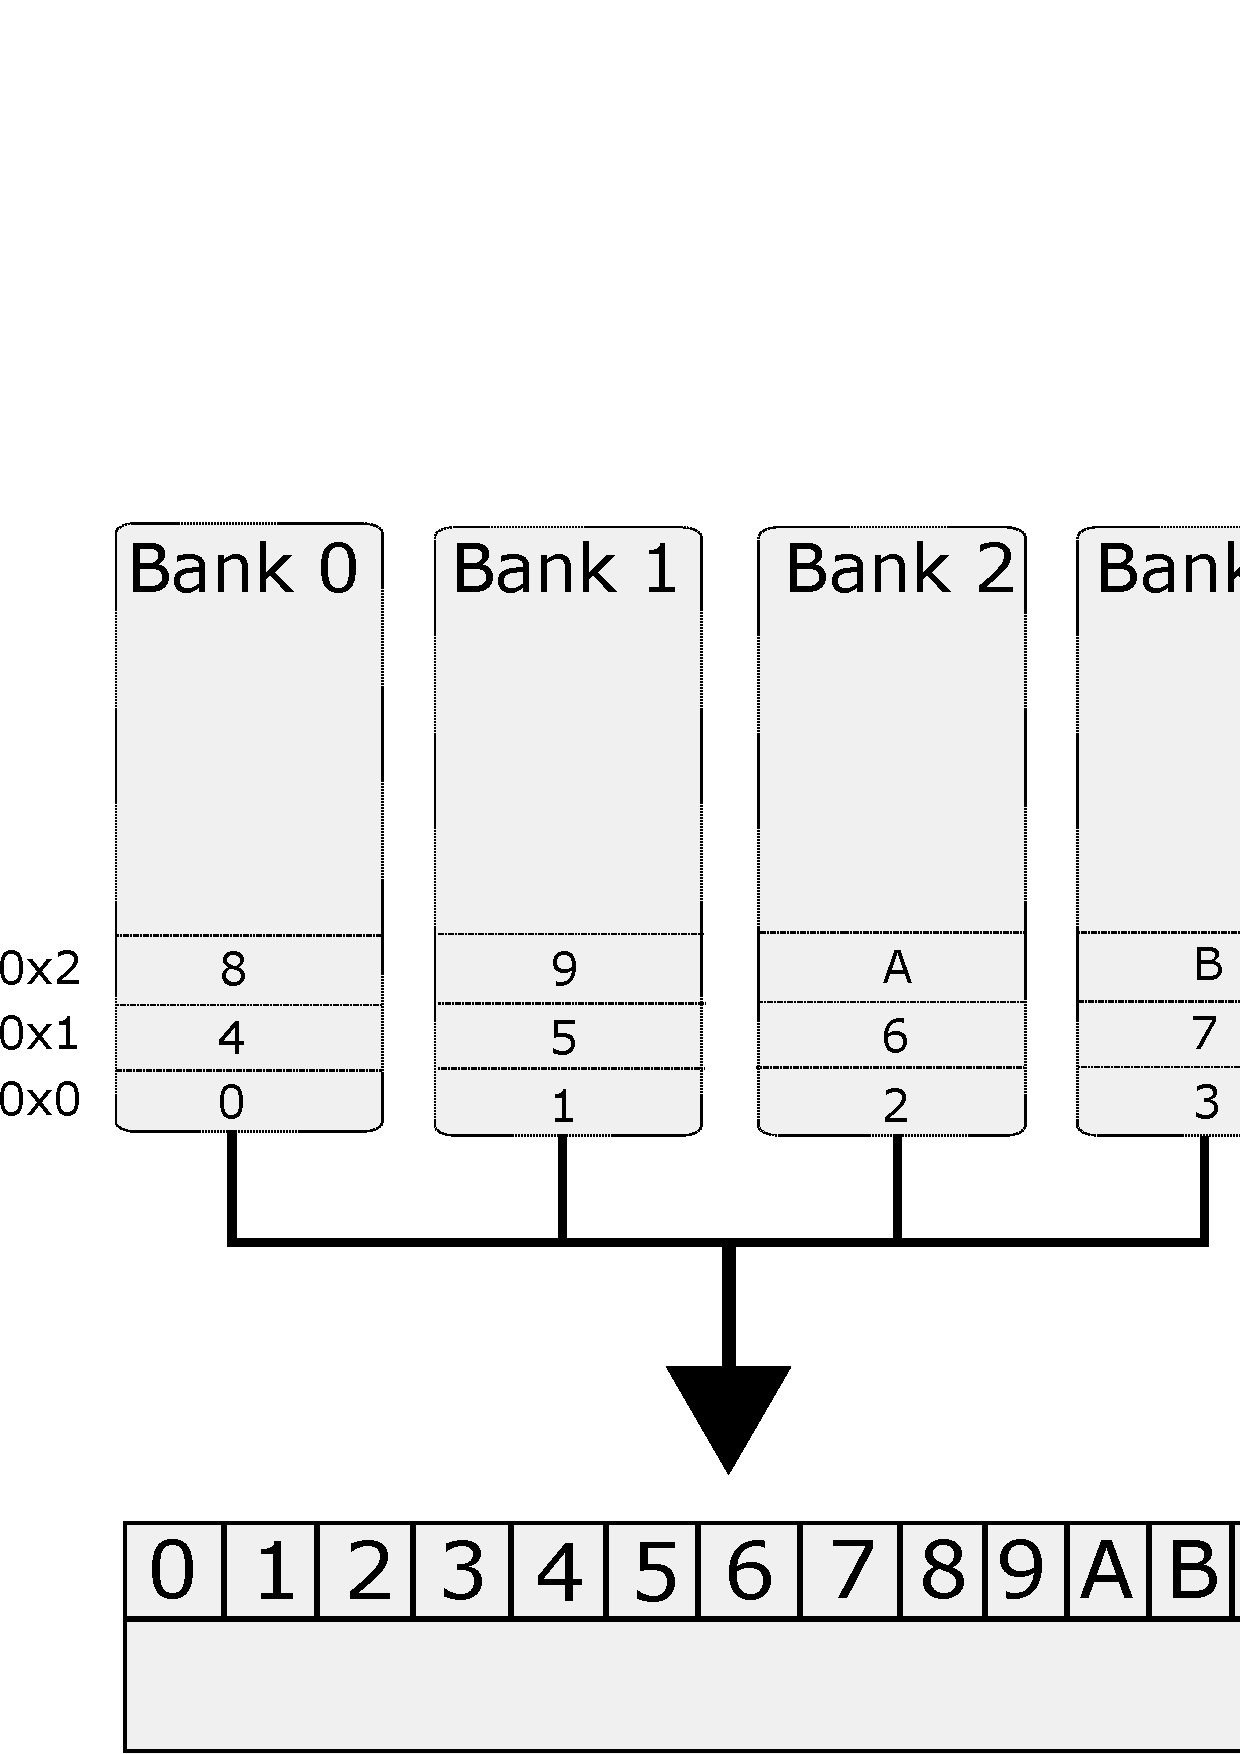
\includegraphics[width=.7\textwidth]{imgs/drawings/scalePost_explanation1.pdf}
 \end{figure}


 Drawing two columns (under pixel 0 and 1) can be done with only one pass using a vga mask set to 3 to write in banks 0 and 1.\\
 \par
 \begin{minipage}{\textwidth}
\lstinputlisting[language=C]{code/pass_0_1.c}
\end{minipage}
\par

 \begin{figure}[H]
 \centering
 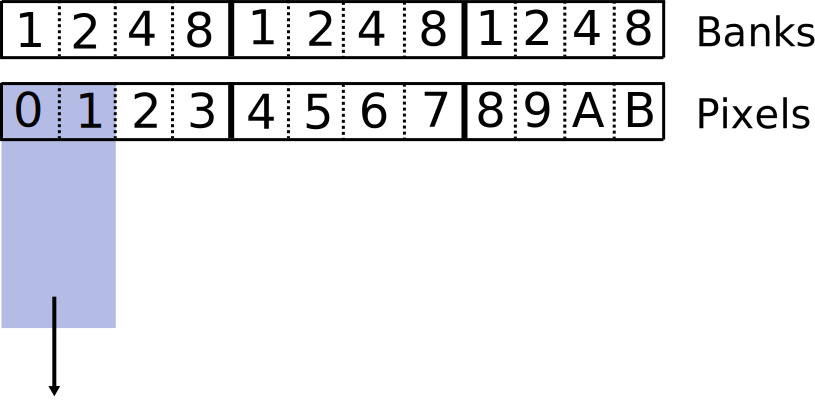
\includegraphics[width=.7\textwidth]{imgs/drawings/scalePost_explanation2.pdf}
 \end{figure}





If the two column are not properly aligned (like columns under pixels 3 and 4), the mask is of no help. Two passes with mask set to 8 and then 1 will be needed.\\
 \par
 \begin{minipage}{\textwidth}
\lstinputlisting[language=C]{code/pass_3_4.c}
\end{minipage}
\par
  \begin{figure}[H]
 \centering
 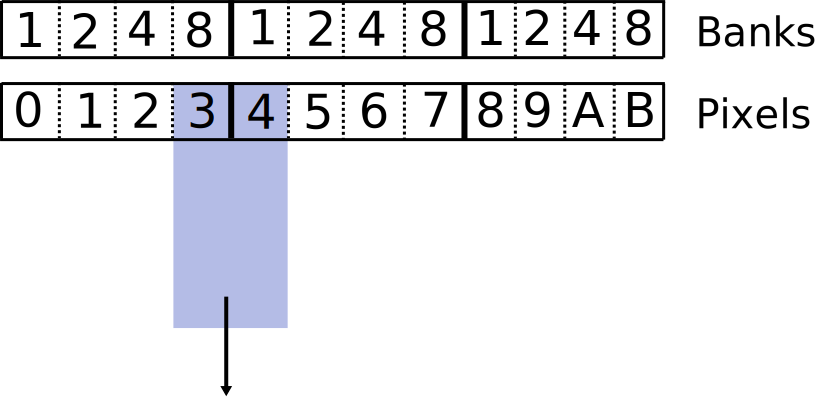
\includegraphics[width=.7\textwidth]{imgs/drawings/scalePost_explanation3.pdf}
 \end{figure}


In the worse case scenario, the engine needs to draw eight column of pixels, under pixels 3,4,5,6,7,8,9 and A. Because of the poor alignment, three passes are needed.\\
 \par
 \begin{minipage}{\textwidth}
\lstinputlisting[language=C]{code/pass_3_A.c}
\end{minipage}
\par
  \begin{figure}[H]
 \centering
 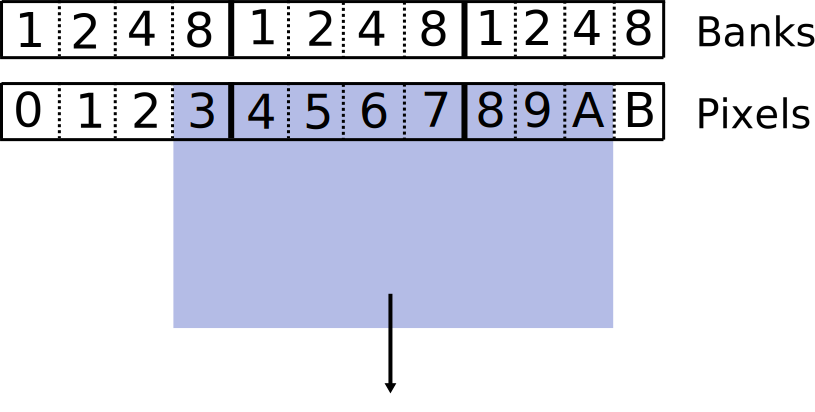
\includegraphics[width=.7\textwidth]{imgs/drawings/scalePost_explanation4.pdf}
 \caption{Three Passes with mask set to: 8,15,14}
 \end{figure}


A better case where two passes allow to draw 6 columns of pixels:\\
 \par
 \begin{minipage}{\textwidth}
\lstinputlisting[language=C]{code/pass_0_5.c}
\end{minipage}
\par
   \begin{figure}[H]
 \centering
 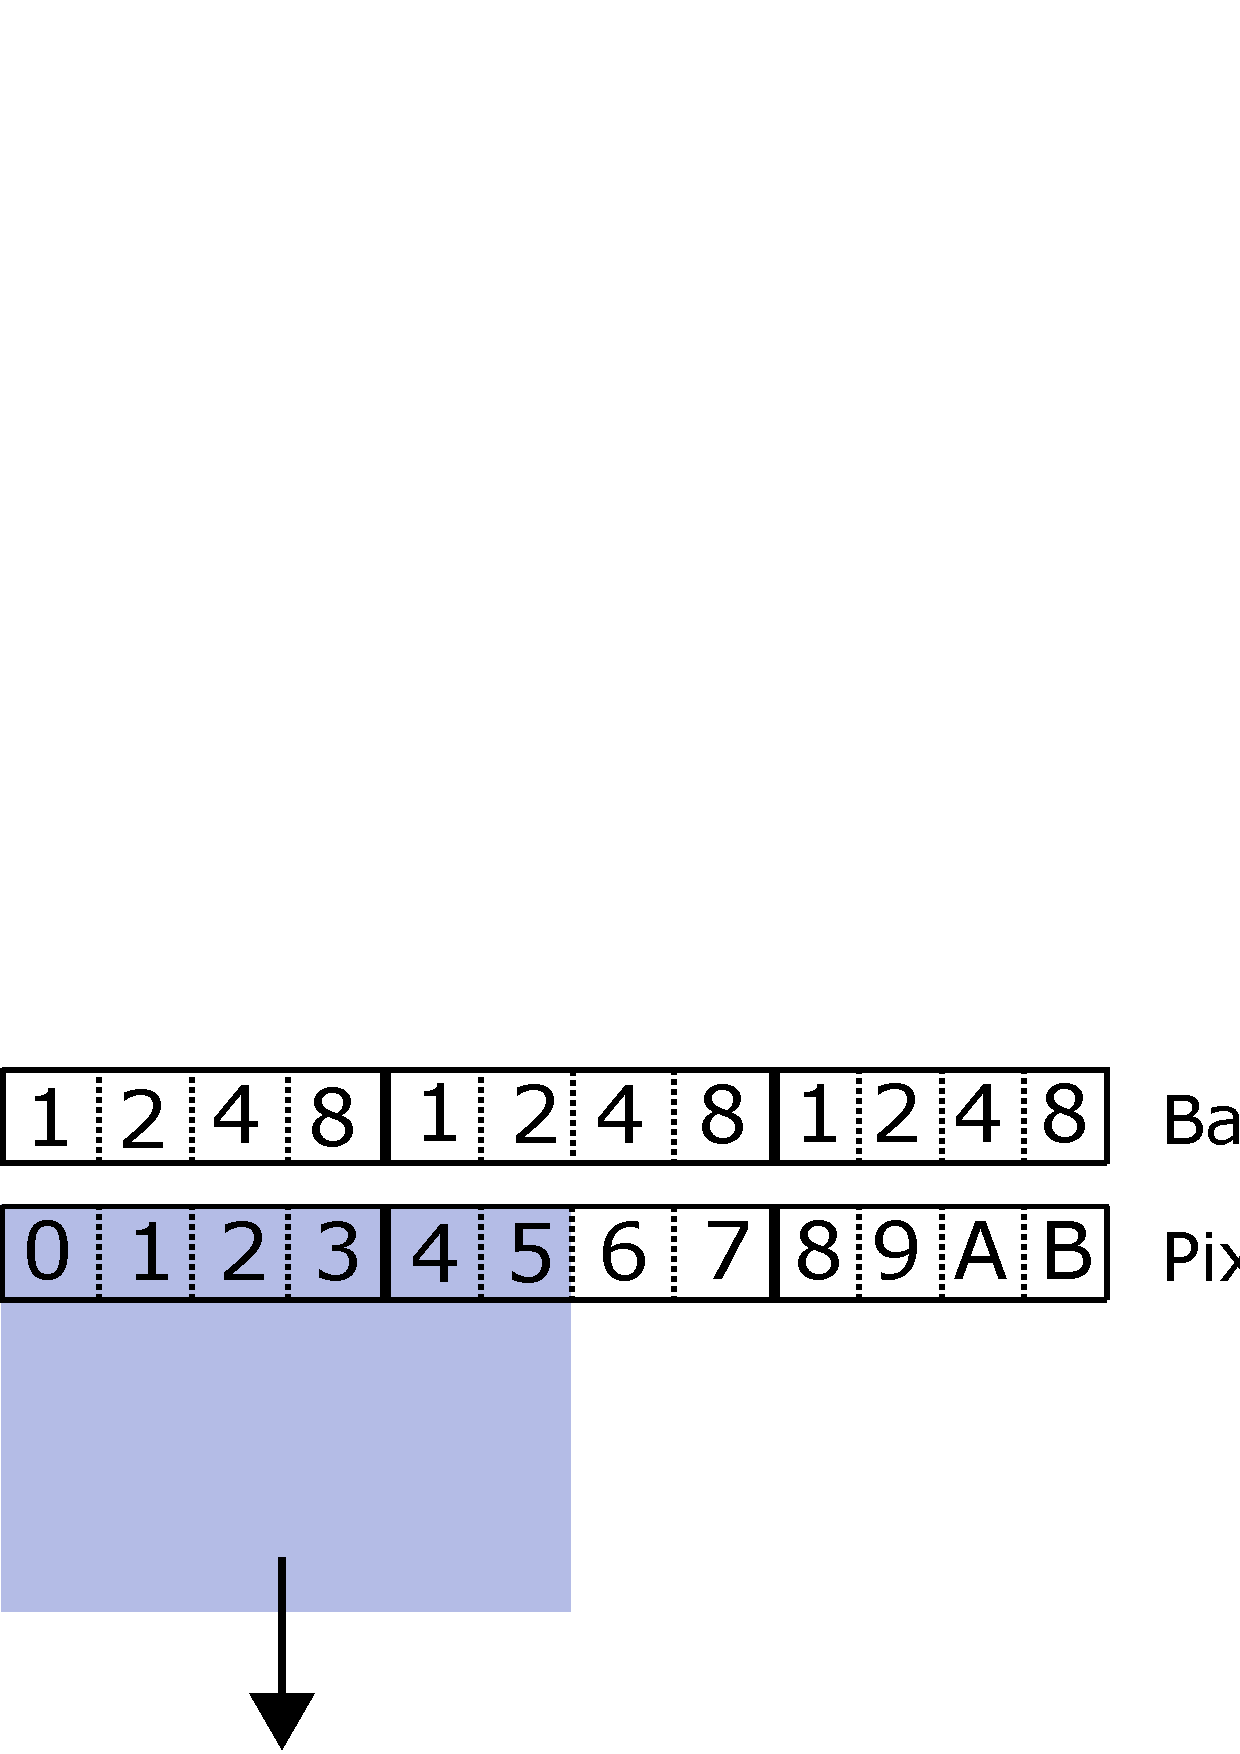
\includegraphics[width=.7\textwidth]{imgs/drawings/scalePost_explanation5.pdf}
  \caption{Two Passes with mask set to: 15 and then 3}
 \end{figure}






To take real case examples, the engine has been modified to draw in pink column of pixels which were written "for free" thanks to the VGA mask manipulation. We can see the performances improvement is significant with 50\% of write operations avoided.

\begin{minipage}{\textwidth}
 \centering
 \scaledimage{0.9}{post_optimization_1_show.png}
\vspace*{0.5cm}\\
 \scaledimage{0.9}{post_optimization_1_pink_show.png}

\end{minipage}



\par

\begin{minipage}{\textwidth}
 \centering
 \scaledimage{0.9}{post_optimization_2_show.png}
 \vspace*{0.5cm}\\
 \scaledimage{0.9}{post_optimization_2_pink_show.png}
\end{minipage}
This technique helps solve the worse case scenario were a lot of pixels have to be written due to the size of the wall. It only really shines when a lot of magnification occurs. For walls far away (minified) this technique doesn't help at all but it doesn't matter since small walls are cheap to render.\\






















\subsubsection{Texturing}
A subtle but extremely efficient trick used to improve quality of the wall rendition is pre-baked light texturing. The wall textures assets are generated twice by the artists: Once lit and once unlit.\\
  \begin{figure}[H]
\centering
 \fullimage{baked_lights_wood.png}
 \end{figure}
\par
  \begin{figure}[H]
\centering
 \fullimage{baked_lights_stone.png}
 \end{figure}
\par
At runtime, upon finding ray-wall intersection, if the ray hit a vertical wall (looking at the map from above) on the Y axis, the engine uses a light texture. If the ray hits an horizontal wall (on the X axis), it uses the darker version of the same texture. It is not obvious at first but with the same scene rendered side by side with and without the effect, the difference is striking.\\
\begin{minipage}{\textwidth}
\begin{figure}[H]
\centering
 \fullimage{backed_off.png}
 \caption{Above: Baked texture off. Below: Backed texture on.}
 \end{figure}

\begin{figure}[H]
\centering
 \fullimage{backed_on.png}
 
 \end{figure}
 \end{minipage}

 





\subsubsection{Door}
Doors are rendered directly via the raycaster. Therefore they have no thickness, that would have been much more complicated to implement.\\
\par
\begin{figure}[H]
 \centering
 \fullimage{door_flat.png}
\end{figure}

\par
Upon hitting a "DOOR" tile, the raycaster consult the \cw{doorposition} array. The raycaster is able to calculate how far along a door is opened and if it should either stop at the door or traverse its.\\

\begin{minipage}{\textwidth}
\lstinputlisting[language=C]{code/door.c}
\end{minipage}

\par 
 \par
\begin{figure}[H]
  \centering
 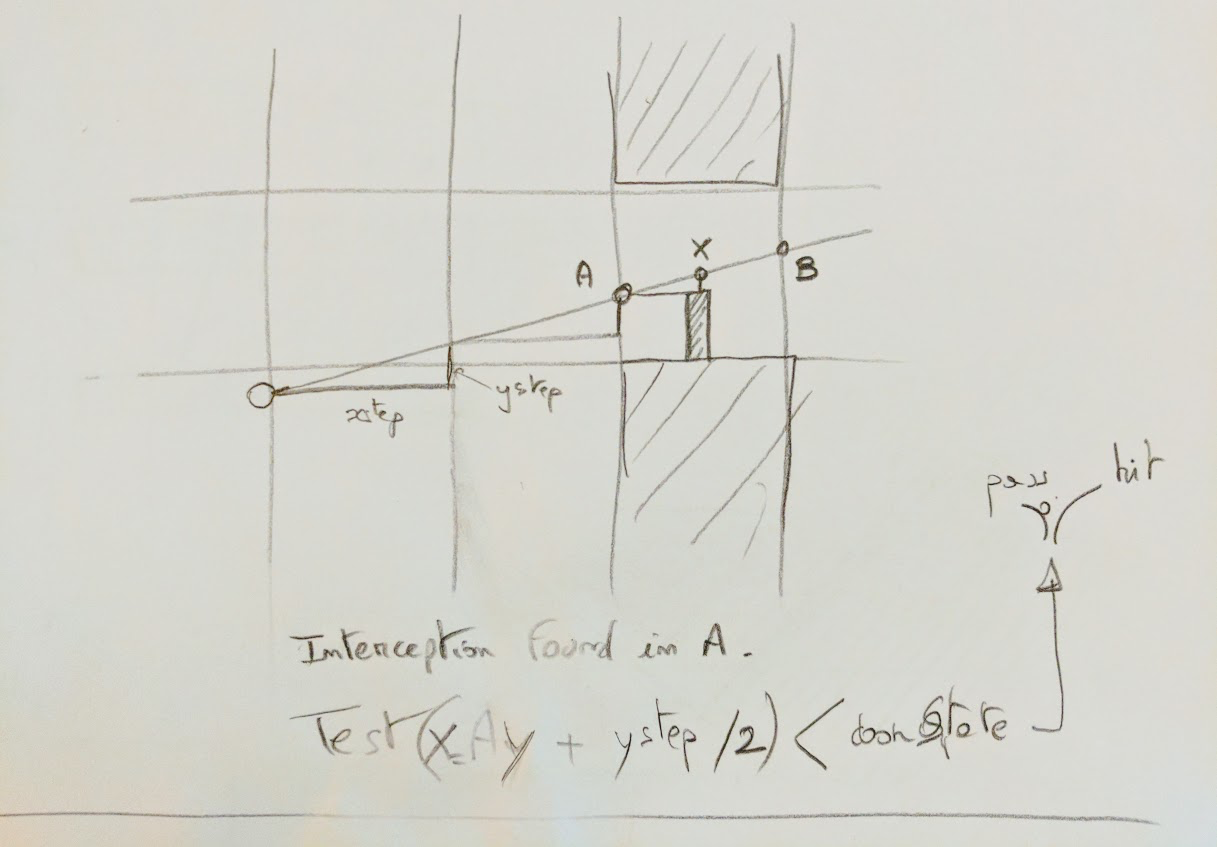
\includegraphics[width=\textwidth]{imgs/drawings/test_door.png}
\end{figure}
\par












\subsubsection{Push walls} 
Push wall are also implemented via the raycaster. Like door, these moving walls are also treated as a special case. If the pushwall has been activated, the raycaster adds an offset to the ray intercept coordinates.

















\subsection{Drawing sprites}
Once the walls are drawn, it is time to render sprites such as enemies, items (ammos, weapons) and decorations (lamps, table, etc). It is a three steps operation.
 \begin{enumerate}
  \item Find which sprites are visible.
  \item Determine which part of the sprite is visible (not hidden by a wall).
  \item Draw what is visible.
 \end{enumerate}



\subsubsection{Visible Sprite Determination}
Building a list of visible sprite is done indirectly by leveraging information gathered by the raycaster relying on the observation that visible sprites are on visible tiles. The raycaster mark all tiles visited by each ray while they travel the map looking for a wall.\\
\begin{figure}[H]
  \centering
  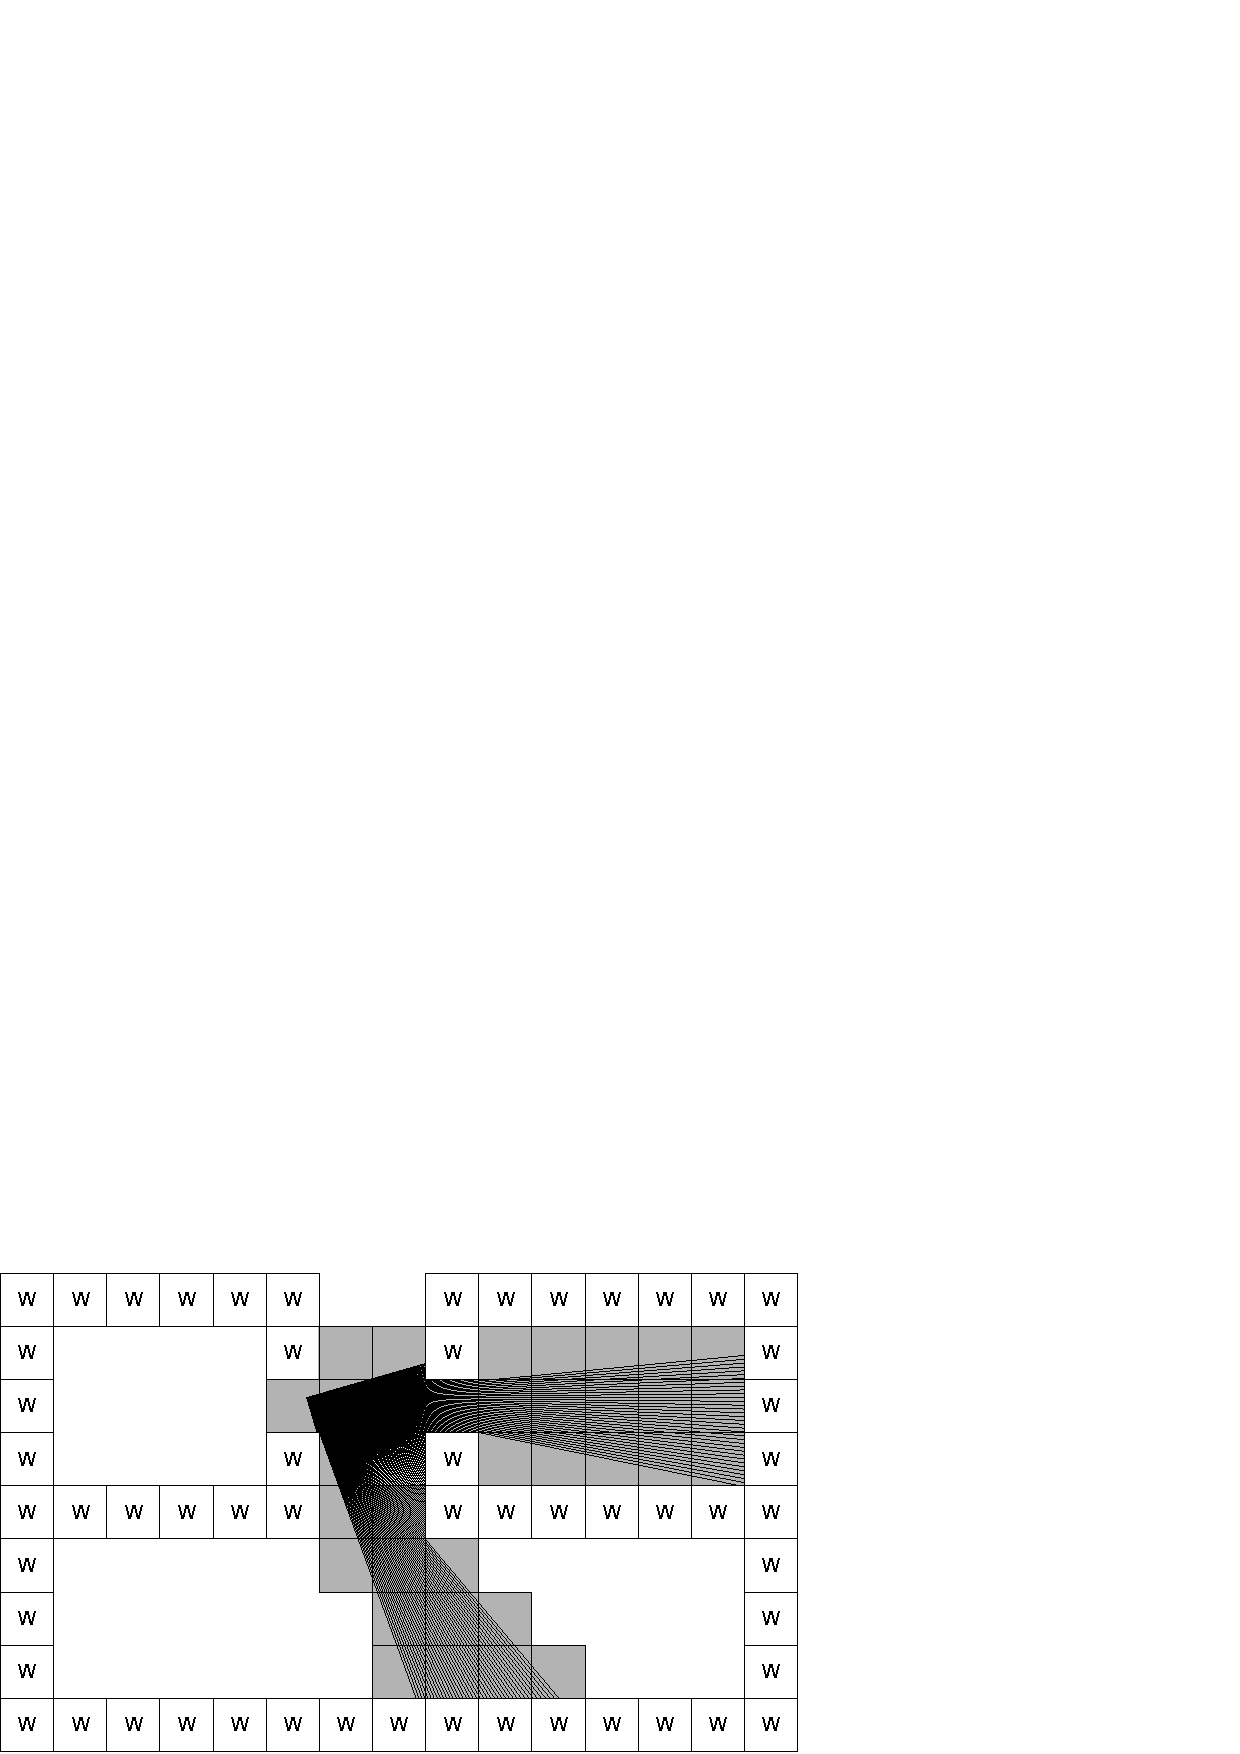
\includegraphics[width=\textwidth]{imgs/drawings/ray_caster_explained/marked_out_room.pdf}
 \caption{Ray cast and visible "spots".} 
\end{figure}
Visible tile tracking is done in the simplest way with a 64x64 boolean array indicating if a tile was visited.\\
\par
\par
\begin{minipage}{\textwidth}
  \lstinputlisting[language=C]{code/spotvis.c}
\end{minipage}
\par

 At the beginning of each frame, the engine clears the array.\\
\par
 \lstinputlisting[language=C]{code/clear_vis_wold3d.c}
 \par
 Note that because register are 2 bytes wide, an array of 64x64=4096 bytes can be zeroed in 2048 iterations.\\
 \par
The ray caster (\codeword{AsmRefresh}) writes \cw{true} in the visible tile array as the ray progresses towards a wall.\\
\par
\begin{minipage}{\textwidth}
  \lstinputlisting[language={[x86masm]Assembler}]{code/mark_vis_wold3d.asm}
\end{minipage}
\par 

The way the visible tile array is used is not the most subtle part of the engine (it runs in $\mathcal{O}(n^2)$ time) but it works well due to the low number of sprites. All sprites on the map are tested for visibility with \cw{spotvis} and their height is calculated. They are all added to an array unsorted. A final double loop draws all sprites from far to near (using sprite height to extract the further on each iteration).\\
\par
\begin{minipage}{\textwidth}
 \lstinputlisting[language=C]{code/build_vis_list.c}
 \end{minipage}
 \par
 




\subsubsection{Rendition}
Each sprites is rendered individually in the function \cw{ScaleShape (int xcenter, int shapenum, unsigned height)}. The sprite is transformed from map space to player space using the same SOH-CAH-TOA math seen in the "Drawing Walls" section.

\par
\begin{figure}[H]
\centering
 \includegraphics[width=\textwidth]{imgs/drawings/spaces.pdf}
 \end{figure}
\par
The X coordinate is used to place a sprite horizontally on the screen and the Y coordinate is used for clipping. Like walls, sprites don't need to be placed vertically since they are drawn in the same 64x64 texels space.\\
\par
  \begin{minipage}{.5\textwidth}
     \fullimage{guard_sprite.png}
  \end{minipage}
   \begin{minipage}{.5\textwidth} 
     \fullimage{wall_texturw.png} 
   \end{minipage}

\par



 As shown in the following screenshot, scaling a vertically centered sprite is enough to give the illusion of perspective.\\
\par
\begin{figure}[H]
 \centering
 \fullimage{drawing_things.png}
\end{figure}

But sprites are special. Walls fill the full 64x64 space and are fully opaque but sprites have transparent parts. As example, the "food" sprite is only 9 texels tall. The lamp sprites uses the full height but the middle is transparent.\\


  \begin{minipage}{.5\textwidth} 
     \fullimage{sprite_food.png} 
   \end{minipage}
  \begin{minipage}{.5\textwidth} 
     \fullimage{light_sprite.png}
   \end{minipage}

\par

\bu{Trivia :} Sprites with a lot of transparency (such as the two shown previously) would later turn out to be a major fillrate issue with the hardware accelerated renderer for the iOS port.\\
\par
\begin{fancyquotes}
Wolfenstein (and Doom) originally drew the characters as sparse stretched columns of solid pixels (vertical instead of horizontal for efficiency in interleaved planar mode-X VGA), but OpenGL versions need to generate a square texture with transparent pixels.  Typically this is then drawn by either alpha blending or alpha testing a big quad that is mostly empty space.  You could play through several early levels of Wolf without this being a problem, but in later levels there are often large fields of dozens of items that stack up to enough overdraw to max out the GPU and drop the framerate to 20 fps.  The solution is to bound the solid pixels in the texture and only draw that restricted area, which solves the problem with most items, but Wolf has a few different heavily used ceiling lamp textures that have a small lamp at the top and a thin but full width shadow at the bottom.  A single bounds doesn't exclude many texels, so I wound up including two bounds, which made them render many times faster. 
\bigskip \\
\textbf{John Carmack - Programmer}
 \end{fancyquotes}

\par












\subsubsection{Clipping}
Like everything in the game, sprites are made of and drawn as columns. Before drawing each columns in a sprite, the engine determines if it is occluded by a wall. This is called clipping and it is an easy step thanks to walls and sprites being in the same 64x64 coordinate system. Once the sprite's position is transformed in player space, the distance Y allows to generate a height. That height is the same calculated for the walls. Therefore to find out if a sprite column if behind a wall, the engine just compare the heights of the wall against the height of the actor.\\
\par
In order to do that, the raycaster keeps tracks of each height calculated for each column in an occlusion array called \cw{wallheight}.\\
\par
\begin{minipage}{\textwidth}
\lstinputlisting[language=C]{code/wallheight_declaration.c}
\end{minipage}
\par
While raycasting the occlusion array is written.\\
\par
\begin{minipage}{\textwidth}
\lstinputlisting[language=C]{code/wallheight_population.c}
\end{minipage}
While drawing sprites, the occlusion array is read. If the height of a wall is greater than a sprite, it means the wall is is front of the sprite and the full sprite rendition is skipped.\\
\par
\begin{minipage}{\textwidth}
\lstinputlisting[language=C]{code/wallheight_usage.c}
\end{minipage}
\par
Since the entire screen is refreshed on the next frame, the occlusion array does not need to be cleared at the beginning of a frame.





\subsubsection{Drawing things}
Sprites rendition benefits from the same optimization we saw in walls (a.k.a: compiled scalers and deferred rendering). But since sprites introduce transparency, the techniques are slightly adjusted.

\subsubsection{Compiled scalers}
Visible sprite column rendition is also done with the compiled scalers. But the scalers cannot be used directly. A compiler scaler draws its speed from its absence of parameters. It is  an unrolled loop hardcoded with x86 instructions to read from a texture 64 texels tall and write/scale a predetermined number of pixels. For example, compiled scaler 112 always reads 64 pixels of texture and magnify it to 134 pixels on the screen.\\
\par
Sprites are stored in a special way to allow tweaked compiled scaler to skip transparency.\\
\par
A sprite is stored as an array of 64 entries. Each entries is a serie of "commands" forming a column. A command features:
\begin{enumerate}
 \item A vertical offset.
 \item A vertical length.
 \item A payload.
 \end{enumerate}
\par
The last command in a column is marked with an offset of \cw{0x00}.\\
\par

\begin{minipage}{.5\textwidth}
\bu{Example :} Column \#25 in the lamp sprite is made of 5 transparent pixels then one sequence of 5 pixels for the lamp:\\
\par
\scaledimage{0.8}{light_sprite_column_head.png}
\par
Then 49 transparent pixels. And finally one sequence of 5 pixels for the light halo.\\
\par
\scaledimage{0.8}{light_sprite_column_bottom.png}
\par
Total: 64 texels. This column is encoded with 2 commands each being: 1 byte offet +  1 byte length + 5 bytes of payload. At the end a payloadless command with length 0x00 marks the end. Total size 17 bytes.\\
 \end{minipage}
\begin{minipage}{.5\textwidth}
\begin{figure}[H]
  \begin{flushright}
     \scaledimage{0.9}{light_sprite_column.png}
   \end{flushright}
\end{figure}
\end{minipage}



 
\par
The idea is to prevent a scaler from consuming the full 64 texels by patching the x86 instructions with an early return instruction \cw{ret}. In order to to that, the code generator also generates patch locations. The \cw{t\_compscale} structure containing a compiled scaler not only features the x86 instruction in \cw{code}, it also features patching offset.\\
\par
\begin{minipage}{\textwidth}
\lstinputlisting[language=C]{code/t_compscale.c}
\end{minipage}
\par
There are 64 patch location per scaler (one for each length of pixels besides 64 desired, stored in \cw{codeofs[]}), allowing to write a \cw{RETF} instruction causing an early return. For each command in a sprite column, the engine looks up how many texels is the command payload, looks up where to patch the scaler, saves the intruction at this location and overwrites it with a \cw{RETF}. After the scaler returns (and the command payload has been rendered), the scaler is unpatched.\\
\par
In the assembly optimized code, note how the engine knows where to patch the code thanks to a \cw{BX} register which point to \cw{codeofs}.
\par
\begin{minipage}{\textwidth}
  \lstinputlisting[language={[x86masm]Assembler}]{code/self_modifying.asm}
\end{minipage}
\par
Patching the scaler is not enough. It only allows to consume less than 64 texels. In order to draw a "hole" properly on screen, the engine also needs to know how many pixels to skip vertically in screenspace before starting the scaler on the next command. This is were the \cw{width[]} array is used. The scaler generator also saved 64 entries to convert sprites transparent height into screen space height.\\


\subsubsection{Deferred rendering}
The same deferred drawing technique we saw for walls is also used for sprites. It is especially powerful when a sprite is magnified.\\

\par
\begin{figure}[H]
 \centering
 \fullimage{magnified_enemy_before.png}
\end{figure}
In this scene, the 64x64 guard sprite is magnified 2.2 times. By zooming in, we see that each column is repeated at least twice. Sometimes three times. It is a perfect optimization case for the VGA planes deferred renderer.\\
\par
A modified version of the engine draw in pink columns which were drawn "for free" thanks to the VGA mask. In this case most column were drawn only once. Magnification was a totally free operation despite more than twice the number of texel written to the screen.\\

\par
\begin{figure}[H]
 \centering
 \fullimage{magnified_zoom.png}
\end{figure}
\begin{figure}[H]
 \centering
 \fullimage{maginfized_zoom_modified.png}
\end{figure}






\subsection{Drawing weapon}
Drawing the weapon at the bottom is straight forward. It uses the same type of rendition for sprite but with specific code where clipping is disabled in function \cw{ScaleShape}. The same compiled scaler and deferred rendition trick are used.














\subsection{A.I}
To simulate enemies, some objects are allowed to "think" and take actions like firing, walking or emit sounds. Those thinking objects are called "actors".\\
\par






Actors are programmed via state machine. They can be aggressive, they can be sneaky or they can be dumb (like when they are a rocket). To model their behavior, all enemies have an associated state:
\begin{itemize}
\item Standing
\item Attack
\item Path
\item Pain
\item Shoot
\item Chase
\item Die
\item Special Boss state
\end{itemize}

With each state are associated \cw{think} and \cw{action} method pointer. There is also a \cw{next} to indicate which state the actor should transition to once it is finished with the current state/action.\\
\par
\begin{minipage}{\textwidth}
\lstinputlisting[language=C]{code/statetype.c}
\end{minipage}
\par


A guard in standing position always stays in the same state (\cw{next} points to itself):\\
\par

\begin{minipage}{\textwidth}
\lstinputlisting[language=C,style=mystyle,basicstyle=\small,morekeywords={statetype, NULL, true, false}]{code/s_grdstand.c}
\end{minipage}
\par
Some state chain are more complex like for example chasing:\\

\par
\begin{minipage}{\textwidth}
\lstinputlisting[language=C,style=mystyle,basicstyle=\small]{code/s_grdchase.c}
\end{minipage}
\par
This example was just for guards. All types of enemies (including bosses) have their own state machine. They often share action (e.g: \cw{T\_Stand} and \cw{T\_Path}) but they also occasionally have their own.\\

\par
What makes enemies interesting is how they go from standing to being aggressive via \cw{T\_Stand}. They have three ways to detect the player:\\
\begin{itemize}
\item Proximity
\item Sight
\item Noise
\end{itemize}
By far the most important stimuli and what makes the player feel like the A.I is smart is the sound.





\subsubsection{Sound propagation}
Early on the game teaches the player that enemies will react to gunfire and seek where the sound was coming from. Sound is an essential part of the experience and propagating it realistically in realtime is hard. A bloodfill algorithm could have been used but that would have been slow. To speed things up, maps are preprocessed. Each room delimits an area. At runtime the engine maintains a matrix of portal connecting areas and updates it when a door opens or closes. Knowing if an enemy can hear the main character gunfire is a simple lookup in a table.

\par
\begin{figure}[H]
 \centering
 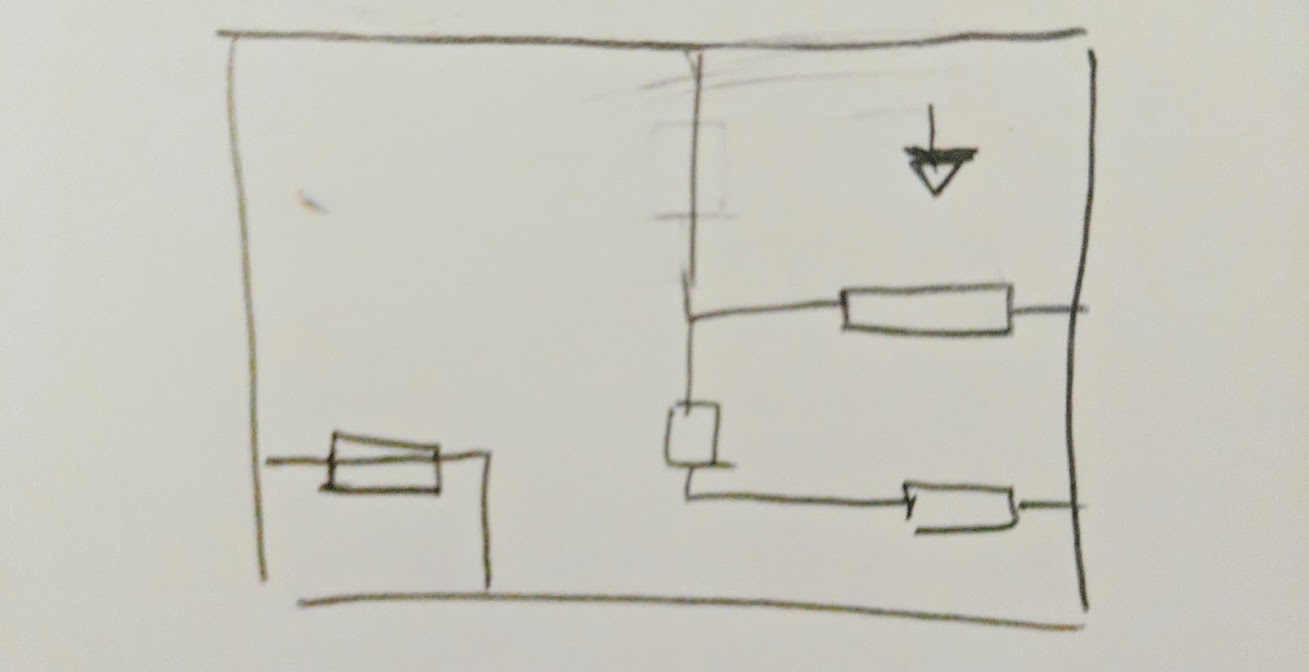
\includegraphics[width=.75\textwidth]{imgs/drawings/sound_area/map.pdf}
 \caption{The map as it is generated with TED5.}
\end{figure}
\par

\par
\begin{figure}[H]
 \centering
 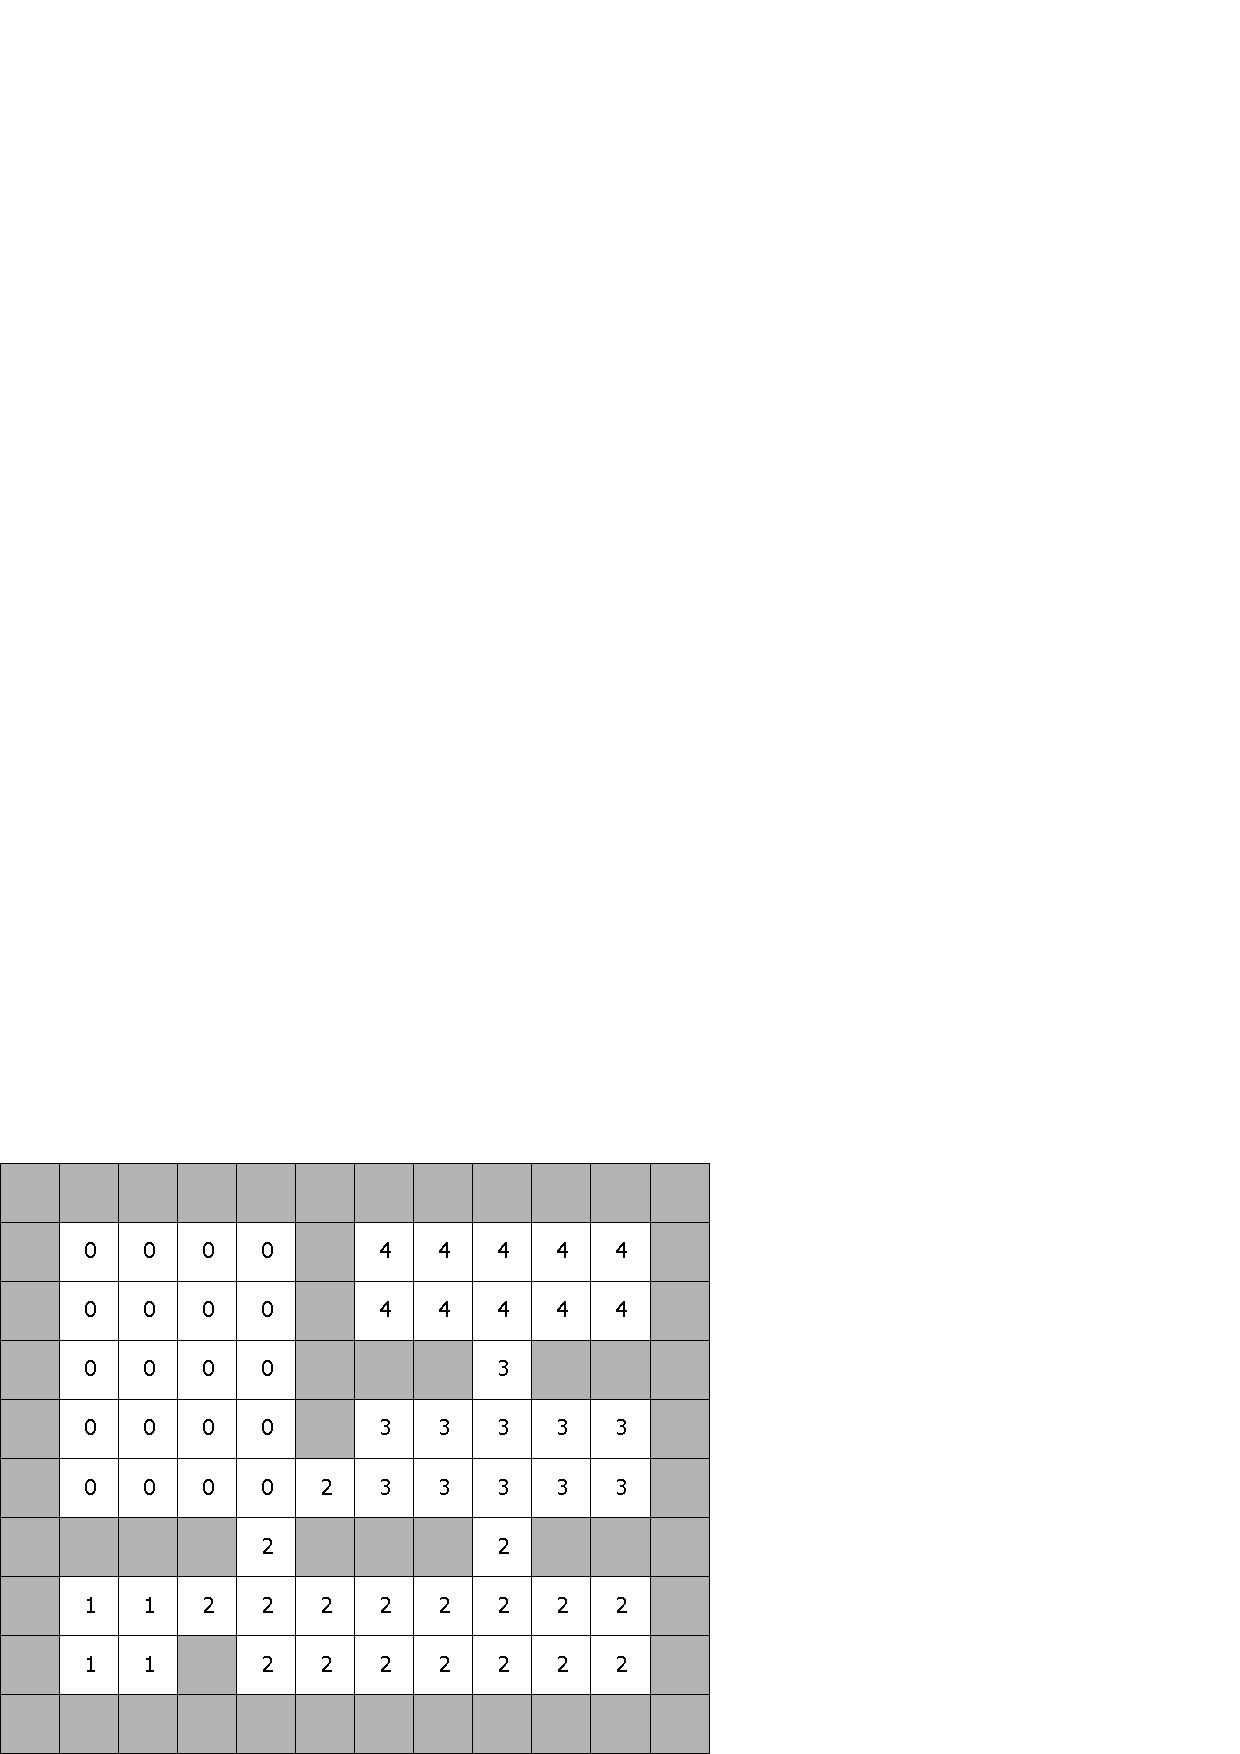
\includegraphics[width=.75\textwidth]{imgs/drawings/sound_area/area.pdf}
 \caption{The same map after is has been pre-processed for audio propagration. Each block belongs to an area.}
\end{figure}
\par



\begin{figure}[H]
 \centering
 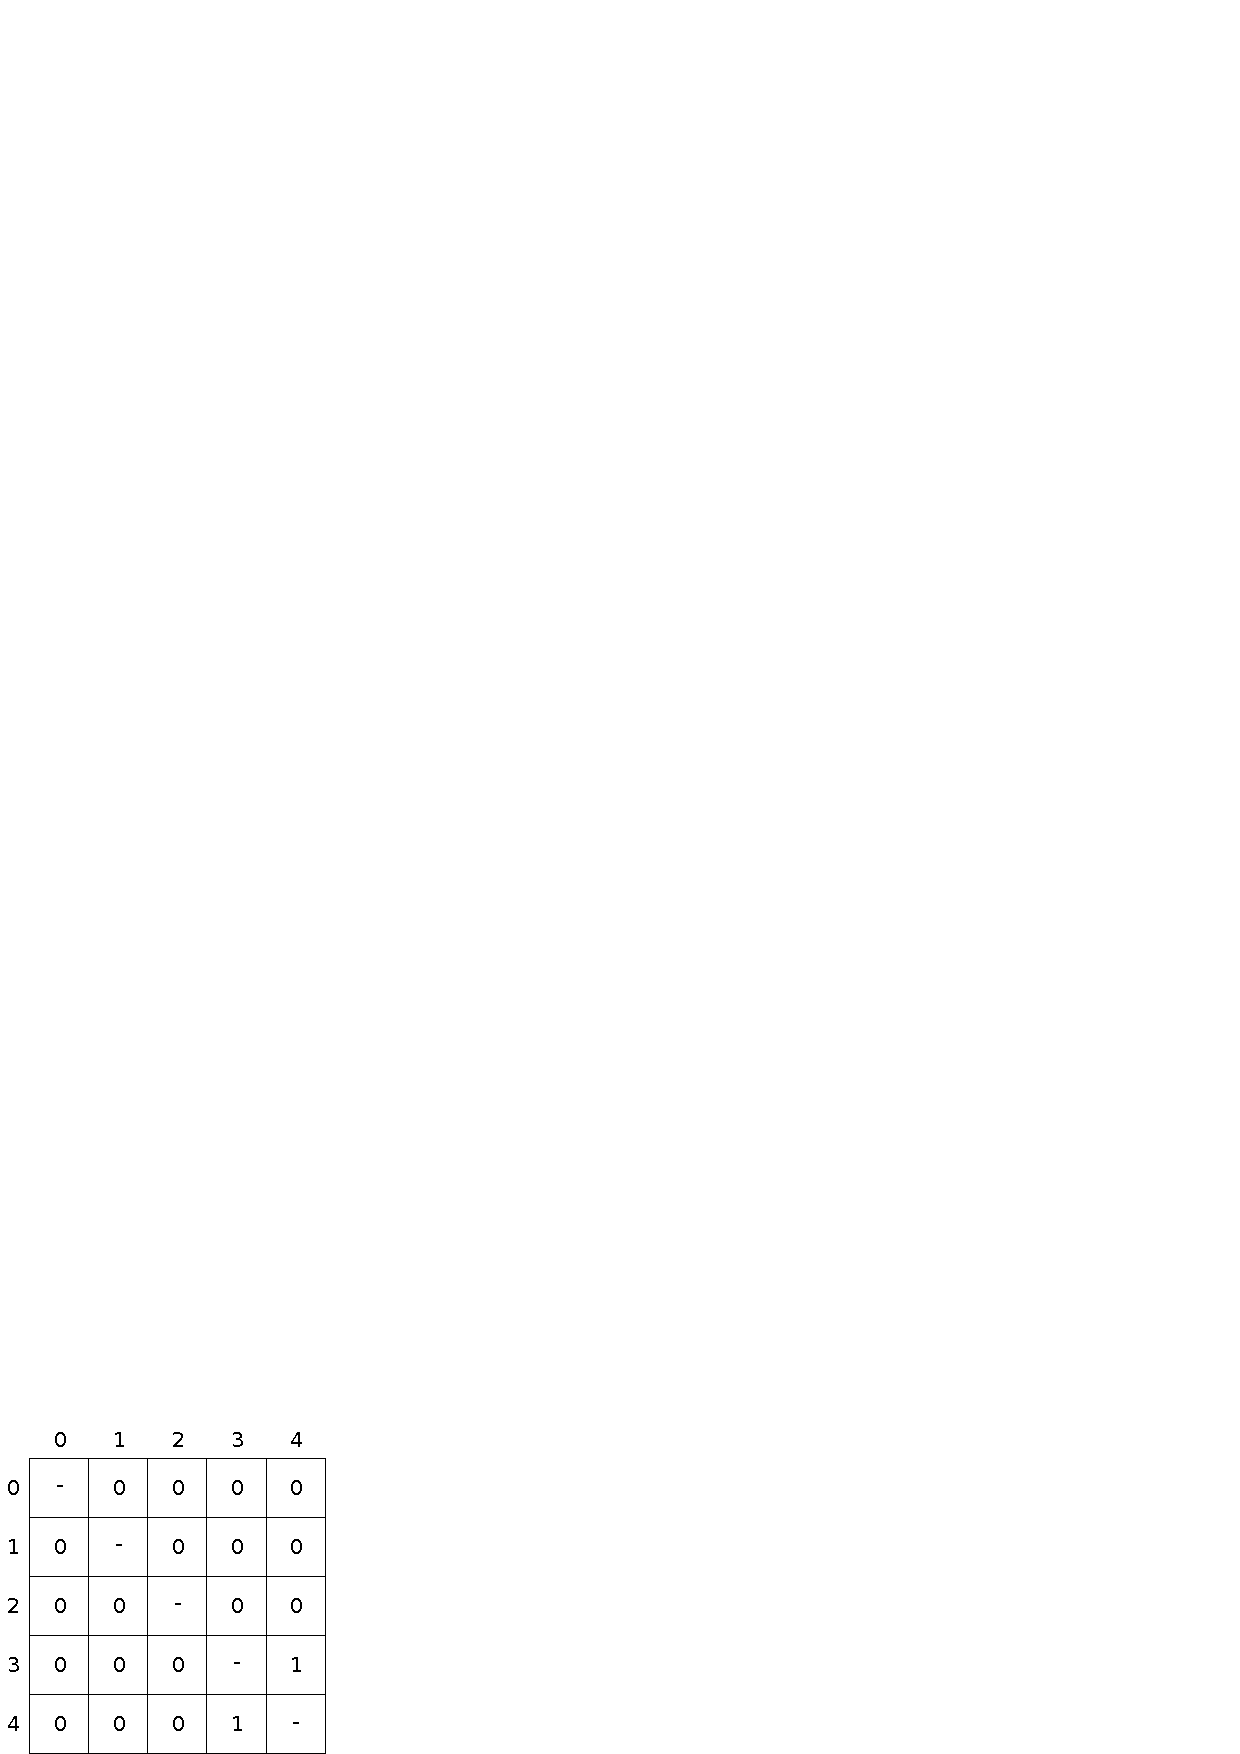
\includegraphics[width=.5\textwidth]{imgs/drawings/soud_propagation/areaconnect.pdf}
\end{figure}
\par
At runtime, the engine maintains a matrix of portal. Each time a door is opened or closed, the array \cw{areaconnect} is updated. 

\par
\begin{figure}[H]
 \centering
 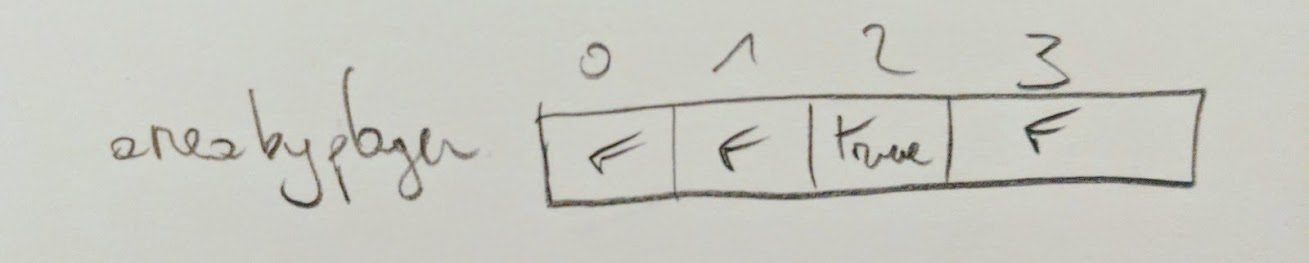
\includegraphics[width=.5\textwidth]{imgs/drawings/soud_propagation/areabyplayer.pdf}
 \caption{Determining if an area can hear the player is a simple lookup in \cw{areabyplayer}.}
\end{figure}
\par
In the source code:\\
\par
\begin{minipage}{\textwidth}
\lstinputlisting[language=C]{code/num_areas.c}
\end{minipage}
\par
\cw{NUMAREAS = 37} seems like a random value. It was likely obtained empirically with the developers bumping it up every time they designed a map which crashed the engine.\\
\par







\subsubsection{Sound non propagation}
Perfect sound propagation is a simplistic model. When a gun is fired, all enemies which can hear it will shout "Achtung!" (Attention!) and converge toward the origin of the sound. That would get old pretty fast. To make things more spicy, the designers introduced a little hack that goes a long way to make the I.A appear smarter than it is.


\par
\begin{minipage}{1\textwidth}
\begin{figure}[H]
 \centering
 \fullimage{ambush/map_unknown.png}
\end{figure}
\par


  \begin{minipage}{0.6\textwidth}
  There is a perfect example early on in the game in map E1M1.\\
  \par At this point in the level, the player have learned that enemies react to gun fire sounds and converge toward its origin. Upon entering this room and dispatching the guard, he/she will naturally assume this is a safe place, a bounded area where no other enemies can be encountered (otherwise they would have showed up by now or at least they would have shouted).
  \end{minipage}
  \begin{minipage}{0.4\textwidth}
  \begin{flushright}
  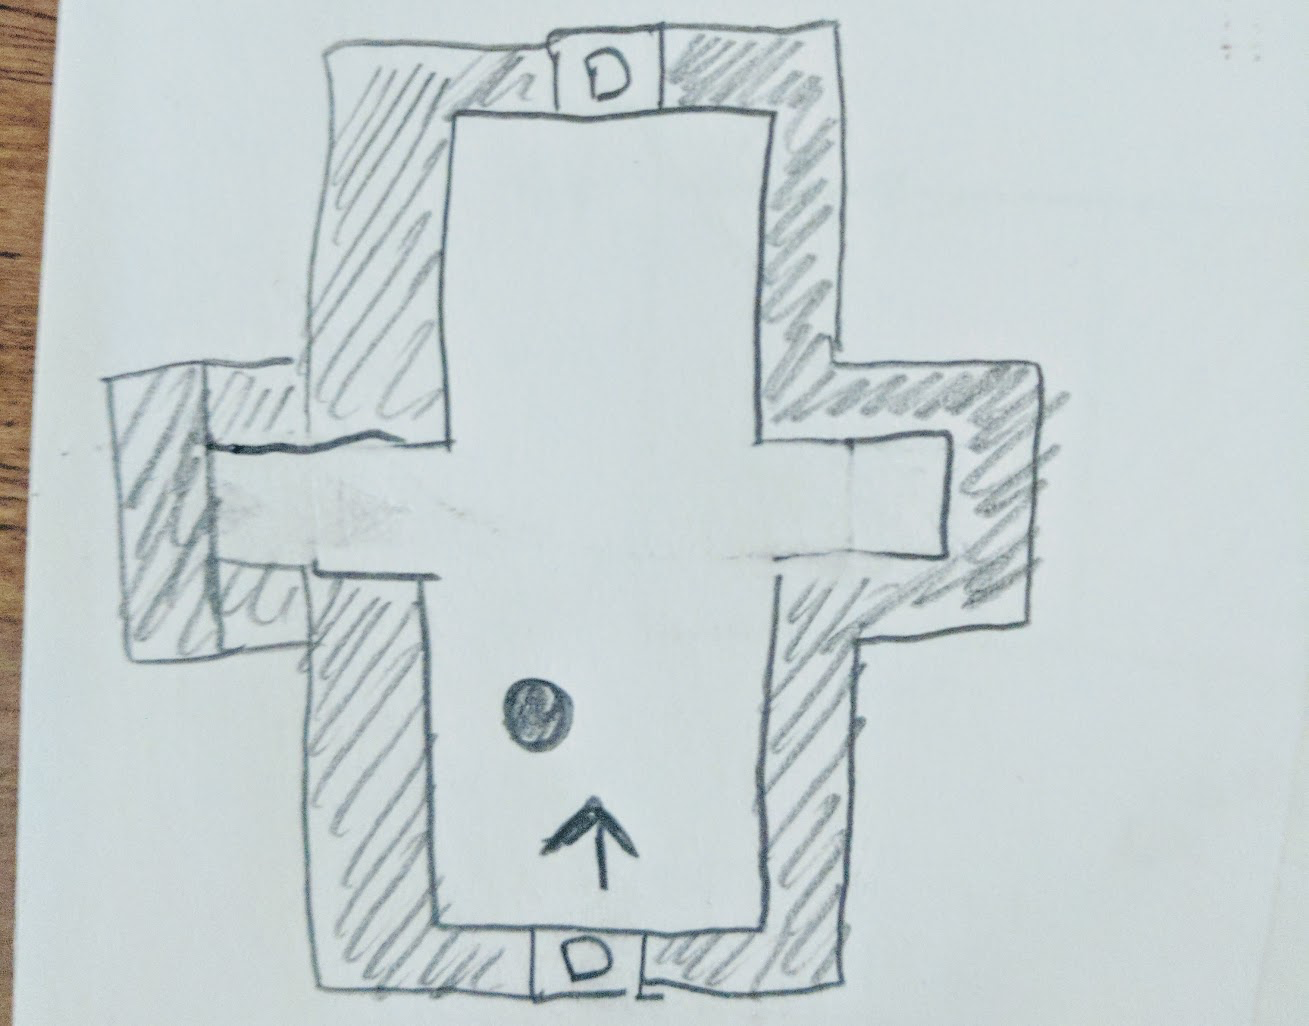
\includegraphics[width=0.9\textwidth]{imgs/drawings/ambush/map_unknown_drawing.pdf}
  \end{flushright}  
  \end{minipage}
\end{minipage}
\noindent
\\


\par
\begin{minipage}{1\textwidth}
  \begin{figure}[H]
   \centering
   \fullimage{ambush/map_ambushed.png}
  \end{figure}
  \par
  \begin{minipage}{0.6\textwidth}
  Feeling safe, she will likely run straight to the door or maybe go left (or worse: right) to see what is in these corners. Surprise ! An enemy was "hiding". This behavior is possible thanks to special tiles marked "AMBUSH" which make the engine not propagate sound to actors standing on these tiles.\\
  \par
   This is probably one of the cheapest feature in the engine yet it results in what most would agree is the soul of the game.
  \end{minipage}
  \begin{minipage}{0.4\textwidth}
  \begin{flushright}
  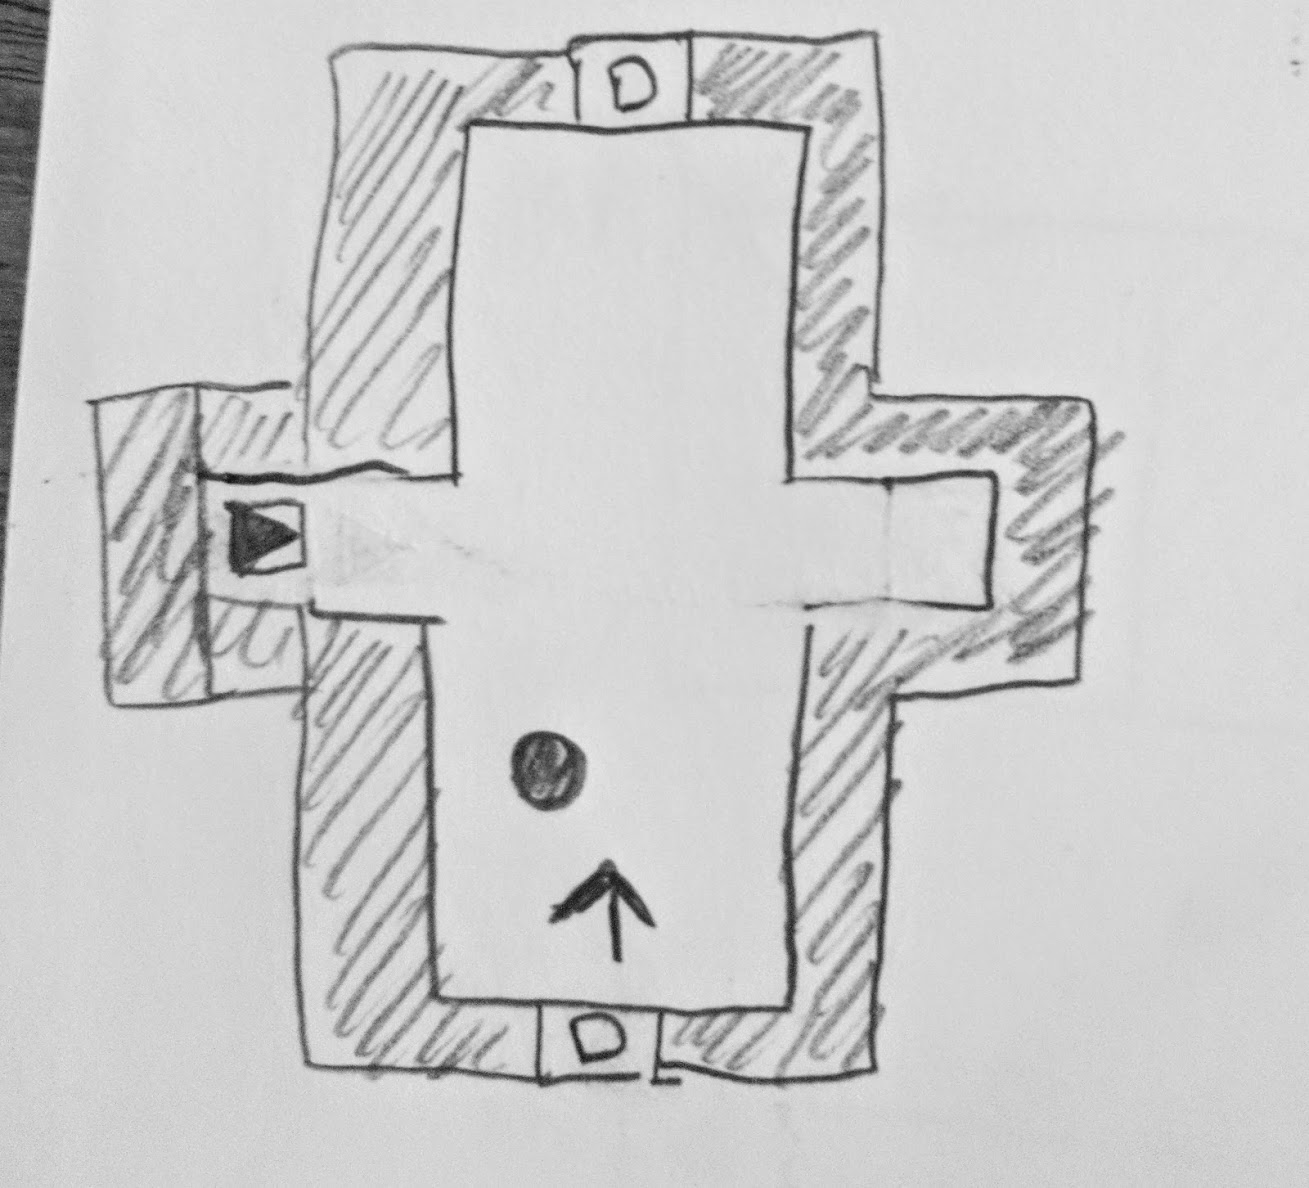
\includegraphics[width=0.9\textwidth]{imgs/drawings/ambush/map_ambushed_drawing.pdf}
  \end{flushright}
  \end{minipage}
\end{minipage}
\noindent
\\


\par

\bu{Trivia :} The ambush behavior is explained in the Hint Book as follow:\\
\par
\begin{fancyquotes}
Each enemy is given specific orders which dictate his actions once he knows of your presence. Some are ordered to immediately attack, while others are trained to act only upon visual contact.
 \bigskip \\
\bigskip \\
\textbf{Kevin Cloud. The Official Hint Manual for Wolfenstein 3D}
 \end{fancyquotes}
\par
\bu{Trivia :} Bug or dedication, a guard on an \cw{AMBUSH} tile will react ONLY to the player sight. Seeing an other actor/dog die right in front of him will not activate him.\\


\subsubsection{Patrolling}
I/A is also augmented with map waypoints for patrolling.\\
\par
\note{Elaborate on how it is done}
\par
\begin{figure}[H]
 \centering
 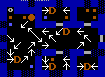
\includegraphics[width=0.98\textwidth]{imgs/drawings/path.png}
\end{figure}
\par

% \subsubsection{Vision reaction}
% \subsubsection{Proximity reaction}
% \subsection{Pursuit and opening doors}
% \subsubsection{Firing at player}






